\section{Methodology} \label{ch4:caseStudy} In this section, we describe the
studied projects, explain how the data was collected, and how we study the types
of delivery delay that are presented in
\hyperref[ch2:deliverydelay]{Section}~\ref{ch2:deliverydelay}.

\subsection{Subjects} \label{ch4:sec:subjects}

In order to study delivery delay, we analyze three subject projects: the
Firefox, ArgoUML, and Eclipse projects, which are from different domains and
sizes. The ArgoUML project is a UML modeling tool that includes support for all
standard UML 1.4 diagrams.\smartfoot{\url{http://argouml.tigris.org/}} The
Eclipse project is a popular open-source IDE, of which we study the JDT core
subproject.\smartfoot{\url{https://www.eclipse.org/}} The Firefox project is a
popular web browser.\smartfoot{\url{https://www.mozilla.org}}

\begin{figure}[t]
	\centering
	\subfloat[Priority values]{
		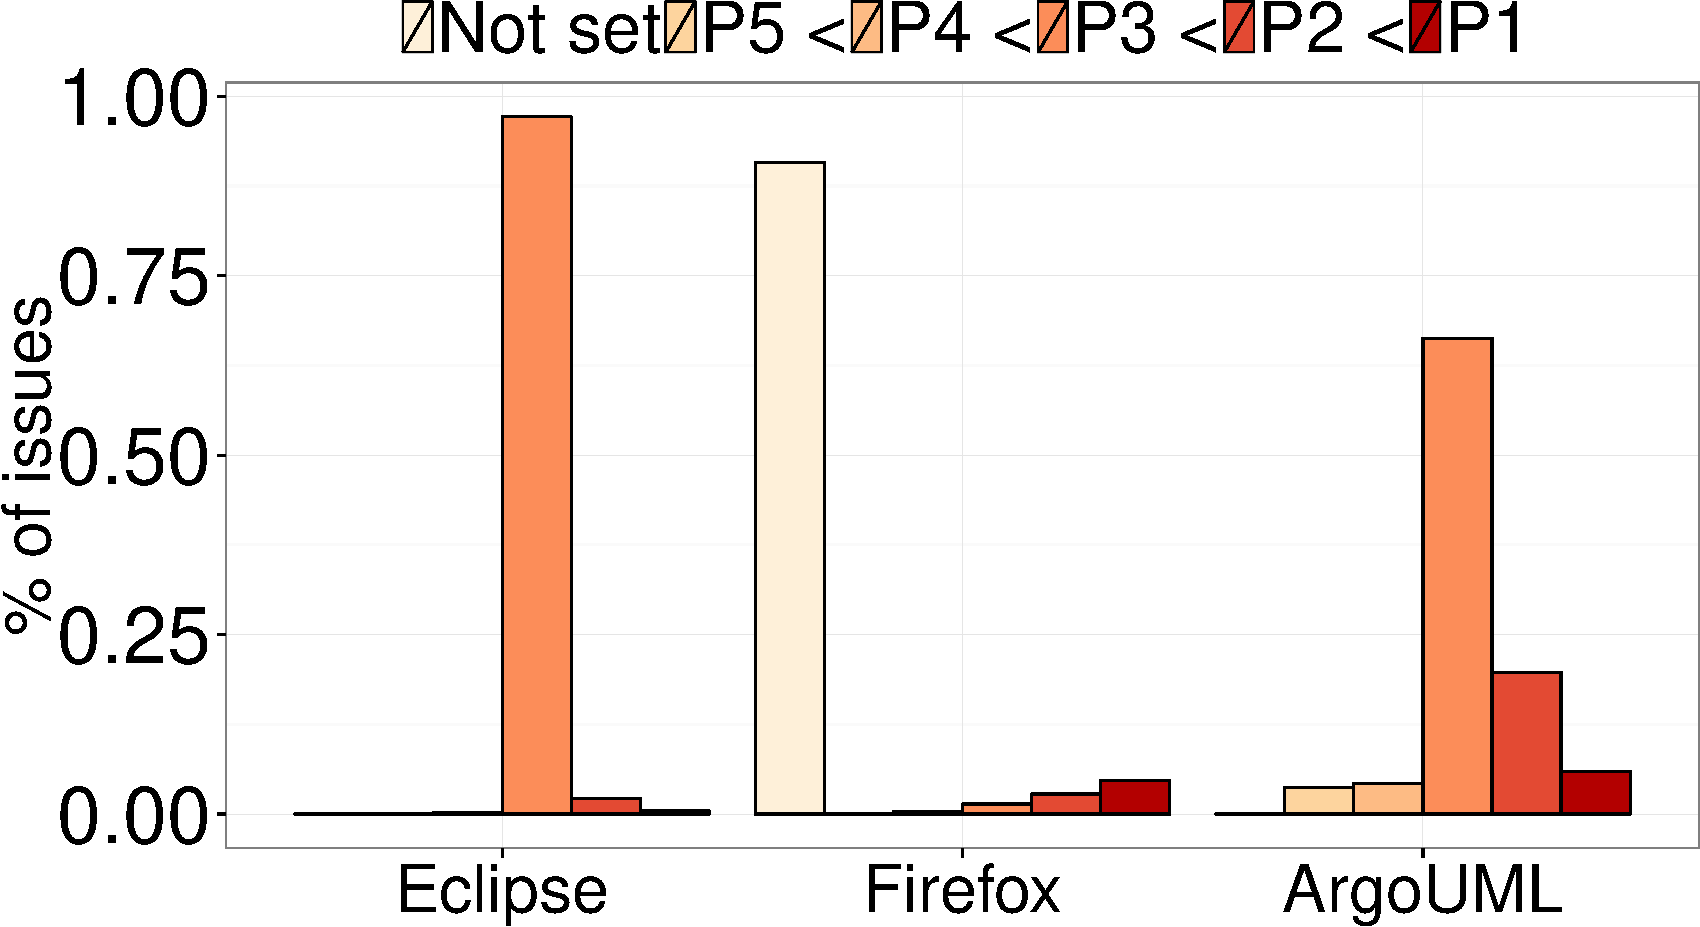
\includegraphics[width=0.60\textwidth,keepaspectratio]
		{chapters/chapter4/figures/issues_per_priority.pdf}
	}

	\subfloat[Severity values. The ArgoUML project does not use the severity field]{
		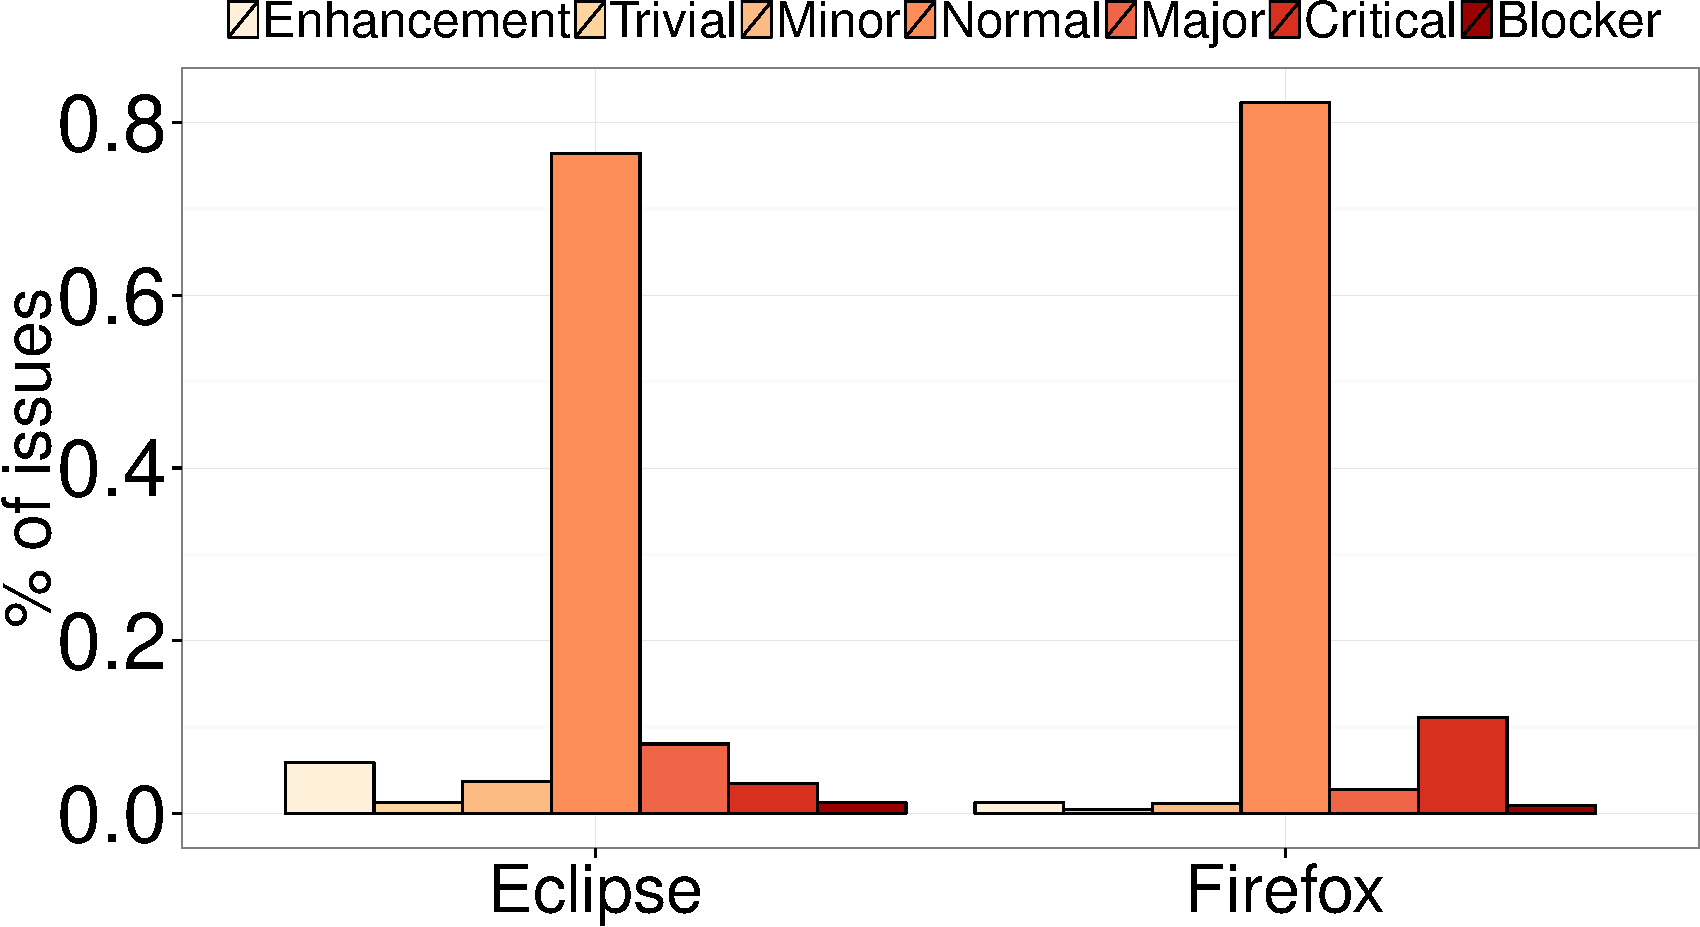
\includegraphics[width=0.60\textwidth,keepaspectratio]
		{chapters/chapter4/figures/issues_per_severity.pdf}
	}

	\subfloat[Fixed issues vs. Not fixed yet]{
		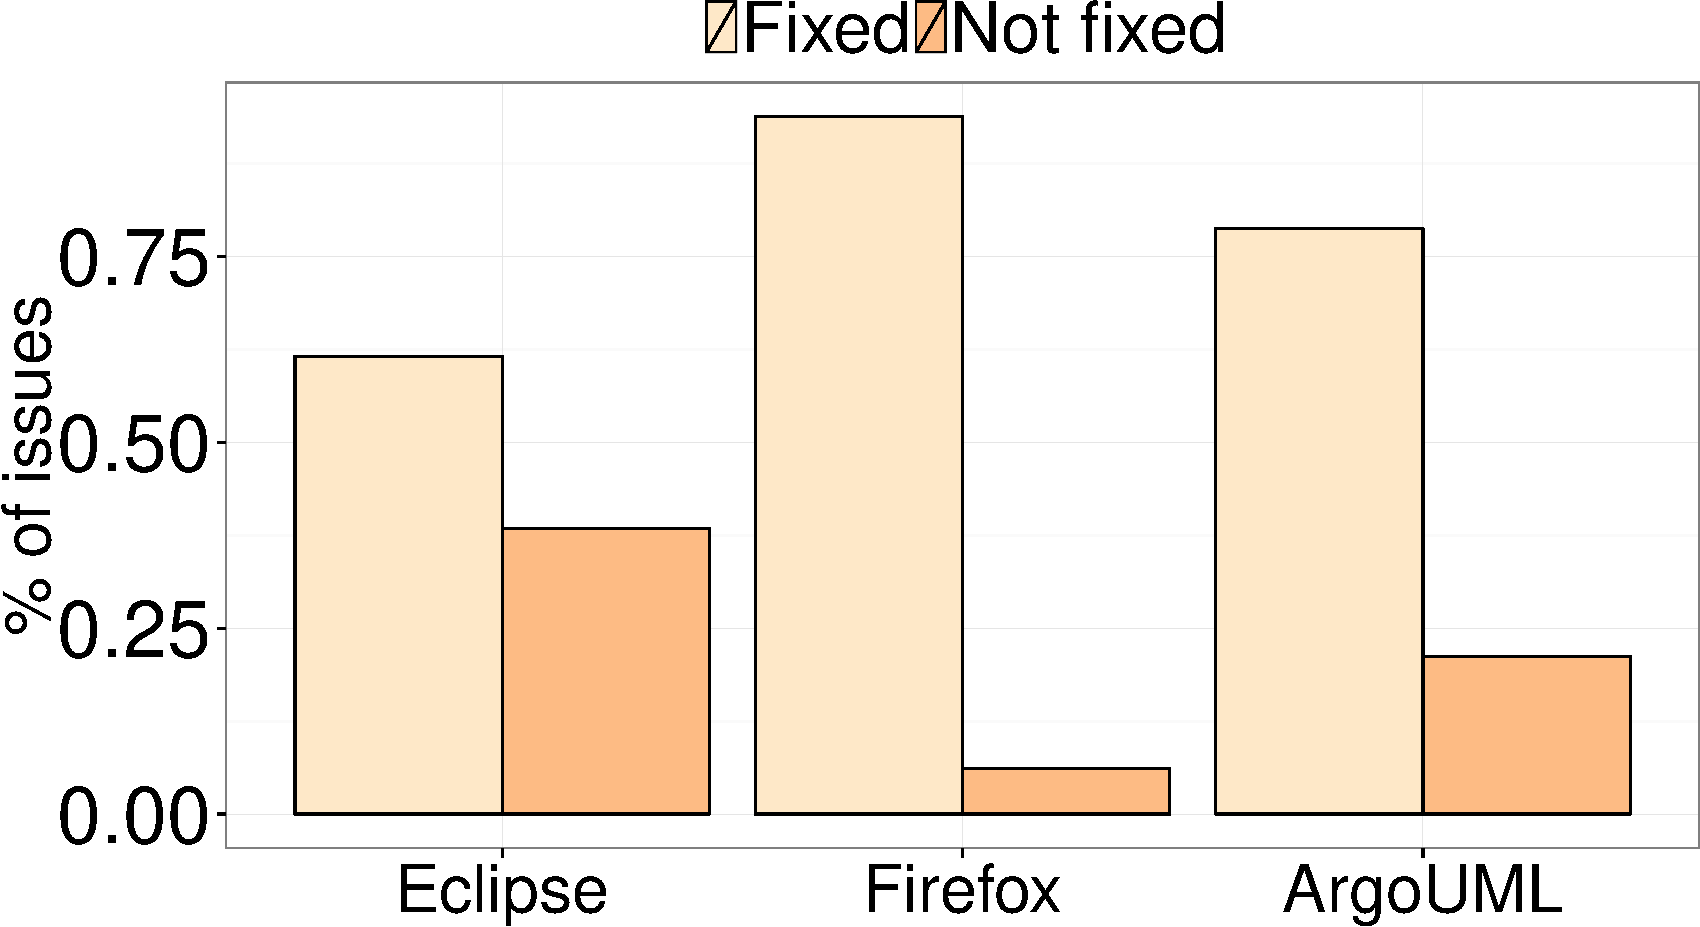
\includegraphics[width=0.60\textwidth,keepaspectratio]
		{chapters/chapter4/figures/neveresolved_resolved.pdf}
	}
	\caption{\textbf{Exploratory analysis of the studied projects.} We
		present the ratio of addressed issues per priority, severity, and the
		ratio of addressed vs. not addressed yet issues (\eg \textit{WONTFIX} or
	\textit{WORKSFORME})}
	\label{ch4:fig:preliminary_studied_system}
\end{figure}

\hyperref[ch4:fig:preliminary_studied_system]{Figure}~\ref{ch4:fig:preliminary_studied_system}
shows an exploratory analysis of our studied projects. We plot the proportion of
issues per priority and severity level, as well as the proportion of issues that
were addressed and not addressed (\eg resolution is \textit{WONTFIX} or
\textit{WORKSFORME}). We observe that for the majority of the issues, the
priority and severity levels remain at the default value. For example, the vast
majority of the priority values are set to P3 (in the Eclipse and ArgoUML
projects) or ``- -'' (in the Firefox project). We also observe that Firefox is
the project with the highest proportion of addressed issues.

\hyperref[ch4:tbl:consideredReleases]{Table}~\ref{ch4:tbl:consideredReleases} shows the
studied period and range of releases, as well as the number of releases and
issue reports. We focus our study on the releases for which we could recover a
list of issue IDs from the release notes. We collected a total of 20,995 issue
reports from the three studied projects. Each issue report corresponds to an
issue that was addressed and could be mapped directly to a release. We present
an overview of the release engineering processes of each studied project below.

\subsubsection*{\textbf{\textit{Eclipse Release Engineering}}}\label{eclipse:releng}

The release engineering of the Eclipse project is composed by {\em
nightly/integration} builds that are followed by {\em milestones} builds and
{\em release candidate} builds. Nightly or integration builds are the least
stable builds and are tested by the early adopters that are following the
eclipse developer mailing lists. For instance, integration builds are not
supposed to be announced through links, blogs, or wikis that are related to the
respective Eclipse
project.\smartfoot{\url{https://eclipse.org/projects/dev_process/development_process.php\#6_Development_Process}} 

{\em Milestone} and {\em release candidate} builds are more stable and can be
announced by external links such as blogs and wikis. The goal is to reach
external early-adopters from outside the developer mailing lists. However, the
external links that refer to such builds should warn that they are not as stable
as official releases. The main difference between a release candidate build and
a milestone build is that a release candidate goes through a rigorous {\em
testing pass}
process.\smartfoot{\url{https://www.eclipse.org/eclipse/development/plans/freeze_plan_4_4.php}}

The testing pass process consists of intensive testing activities that are
performed by the development team and community to find regression and {\em
stop-ship} bugs. In case stop-ship bugs are found late in the process, the
release schedule may be slipped to accommodate the fixes for such
bugs.\footnotemark[15]

After the testing pass stage, a {\em fixing pass} stage starts. The fixing pass stage
consists on prioritizing and fixing the most severe bugs that are found at the
testing pass stage. By the end of a fixing pass stage, another release candidate is
produced. The process of performing testing passes and fixing passes is done through
several iterations (\ie many release candidates are produced). 

The last release candidate is submitted to a {\em code freeze} stage. The {\em
code freeze} is a period at which the rules to integrate changes in the software
project becomes more strict. For instance, new changes may be integrated only if
they are solving special requirements such as translations or documentation
fixing.\footnotemark[15] Such a period is important because it helps the
development team to stabilize the project just before creating an official
release.

Official releases are categorized as {\em major}, {\em minor}, and {\em service} 
releases.\smartfoot{\url{https://www.eclipse.org/projects/handbook/\#release}}
Major releases include API changes. Minor releases add new functionalities but
are compatible with the API of prior versions. Finally, service releases include
bug fixes only (\ie without significant addition of new functionality). Both
major and minor releases have to pass through a {\em release review} process. A
release review aims at getting feedback about the release cycle that was
performed. The main goal is to find areas of improvement and if the development
process is being open and
transparent.\smartfoot{\url{https://www.eclipse.org/projects/handbook/\#release-review}}

\subsubsection*{\textbf{\textit{Firefox Release Engineering}}}\label{firefox:releng}

The release engineering process of the Firefox project uses a {\em rapid} (or
{\em a short}) release cycle, \ie a release cycle of 6 weeks duration. In
addition, the process also include {\em pipelining} releases (also known as {\em
release training}) as a means to stabilize the official release, so that they
can be shipped to end users.

The pipelining process develops releases through several channels.
As the release progresses through these channels, the stability of the release
increases and less severe bugs are more likely to be uncovered. The Firefox project team
uses four channels to develop releases: {\em NIGHTLY}, {\em AURORA}, {\em BETA},
and {\em RELEASE}
channels.\smartfoot{\url{http://mozilla.github.io/process-releases/draft/development_overview/}}

The NIGHTLY channel produces a release every night (\ie as soon as features are
ready). This nightly release is built from the {\em mozilla-central} repository and has
the lowest stability of the
channels.\smartfoot{\url{https://hg.mozilla.org/mozilla-central/}}
The AURORA channel produces a release every six weeks. However, some new
features may be disabled if they are not stable enough. At the end of the cycle
of the AURORA channel (the sixth week), the release management team decides which
of the issues that were further stabilized are good enough to migrate to the BETA
channel. Again, the goal of the BETA channel is to stabilize the new features
and disable the features that are not stable enough by the end of the cycle.
Finally, the features that are stable enough to survive at the BETA channel are
moved further to the RELEASE channel, from which an official major release is
produced.\footnotemark[18]

In the Firefox release engineering process, the release schedule is not slipped
to accommodate issues that are not stable enough by the end of the release
cycle. Instead, the development team holds such issues back to be shipped in
future releases when a greater degree of stability is achieved.\footnotemark[18]
Also, an issue may be integrated directly into the AURORA or BETA channels (\ie
the issue is {\em uplifted}), but such cases are exceptions (\eg very critical
security issues that must be released as soon as possible).\footnotemark[18] 

The Firefox project also ships {\em Extended Support Releases} (ESR) that are
based on prior official Firefox releases. ESRs are meant to institutions such as
business organizations, schools, and universities that need to manage their
Firefox desktop client. ESRs provide one year of support for security and bug
fixes of prior Firefox official releases. ESRs are important for organizations
that are not able to follow the fast pace that the Firefox major release
evolves.\smartfoot{\url{https://www.mozilla.org/en-US/firefox/organizations/faq/}}

\subsubsection*{\textbf{\textit{ArgoUML Release Engineering}}}\label{argouml:releng}

In the ArgoUML release engineering process, there are five types of releases:
{\em development}, {\em alpha}, {\em beta}, {\em stable}, and {\em stable patch}
releases. {\em Development} releases are the least stable, while {\em stable}
releases are the official releases that are intended to be widely adopted by the
users.\smartfoot{\url{http://argouml.tigris.org/wiki/How_to_Create_a_Stable_Release}}

{\em Development} releases are generated during the {\em development} stage.
The {\em development} stage may take from one to several months. During this
stage, the development team strives to produce a {\em development} release each
month. {\em Development releases} are not supposed to be used by end users. Such
releases are only advertised to users if there is a purpose of recruiting new
developers to implement and test new features.\footnotemark[21]

After the {\em development} stage, the {\em alpha} stage starts. The {\em
alpha} stage is also referred as the {\em enhancement freeze} point. All of the
enhancements that are not stable enough before the start of the {\em alpha}
stage are not included into the {\em stable} release. According to the ArgoUML
documentation, the {\em alpha} stage usually takes a ``{\em couple of weeks}''
and the development team strives to make a release each week.\footnotemark[21]

The {\em alpha} stage is followed by the {\em beta} stage. The {\em beta}
stage is also referred as the {\em bug-fix freeze} point, \ie all of the (less
severe) bug-fixes that could not be completed before the start of the {\em beta}
stage are omitted from the {\em stable release}. Such remaining bugs are listed
on the ``{\em known problems}'' document that is to be published along with the
{\em stable} release. {\em Beta} releases are more stable than {\em alpha} releases
and are also referred as {\em release candidates}. For instance, {\em beta}
releases should not contain high priority bugs (\ie issues for which the
priority is either P1 or P2).  The {\em beta} stage is supposed to last for a
couple of weeks with a {\em beta} release being generated each week. Finally,
the {\em beta} stage is marked by intense testing activities after each release
candidate. When the team is confident that the {\em beta} release is stable
enough, the official {\em stable} release is generated with no code changes from
the last {\em beta} release.\footnotemark[21]

The last type of ArgoUML release is the {\em stable patch} release. {\em Stable
patch} releases are generated if critical bugs are found after the publication
of the {\em stable} release. The {\em stable patch} release contains the fixes
for the eventual critical bugs that are found upon {\em stable}
releases.\footnotemark[21] The ArgoUML team strives to ship a {\em stable}
release every 8
months.\smartfoot{\url{http://argouml.tigris.org/wiki/Strategic_Planning}}

\subsection{Data Collection}

\hyperref[ch4:fig:overview]{Figure}~\ref{ch4:fig:overview} provides an overview of our
data collection approach---how we collect and organize the data in order to
perform our empirical study. We create a relational database that describes the
\DIFdelbegin \DIFdel{integration of fixed }\DIFdelend \DIFaddbegin \DIFadd{delivery of addressed }\DIFaddend issues in the studied projects. We briefly describe our
data sources, and each step that are involved in the database construction process. 

\subsubsection*{\DIFdelbegin \textbf{\textit{\DIFdel{Step 1: Fetch integrated issue IDs}}%DIFAUXCMD
}%DIFAUXCMD
\DIFdelend \DIFaddbegin \textbf{\textit{\DIFadd{Step 1: Fetch delivered issue IDs}}}\DIFaddend }


\begin{table}
	\footnotesize
	\caption{\textbf{Overview of the studied projects.} We present the number
	of studied releases, issues, the studied period and the median time
	between releases.}
	\label{ch4:tbl:consideredReleases}
	%\resizebox{\columnwidth}{!}{
	%\begin{tabular}{L{1.45cm}C{2.5cm}C{1.5cm}C{0.7cm}R{0.75cm}R{2.25cm}}
	\begin{tabular}{L{1.65cm}C{2.5cm}C{1.5cm}C{1.0cm}R{2.45cm}R{4.25cm}}
		\hline 
		\centering{\textbf{Project}} & \textbf{Studied period} &
		\textbf{Releases} & \centering{\textbf{\# of \newline releases}}
		& 
		\centering{\textbf{\# fixed issues}} & \centering{\textbf{Median
time between releases (weeks)}}\tabularnewline
		\hline 
		\hline 
		\textbf{Eclipse (JDT)} & 03/11/2003 - 12/02/2007 & 2.1.1
		- 3.2.2 & 11 & 3344 & 16\tabularnewline
		\hline 
		\textbf{Firefox} & 05/06/2012 - 04/02/2014 & 13 - 27 &
		15 & 3121 & 6\tabularnewline
		\hline 
		\textbf{ArgoUML} & 18/08/2003 - 15/12/2011 & 0.14 - 0.34
		& 17 & 14530 & 26 \tabularnewline
		\hline 
	\end{tabular}
\end{table}

\begin{figure}
	\centering
	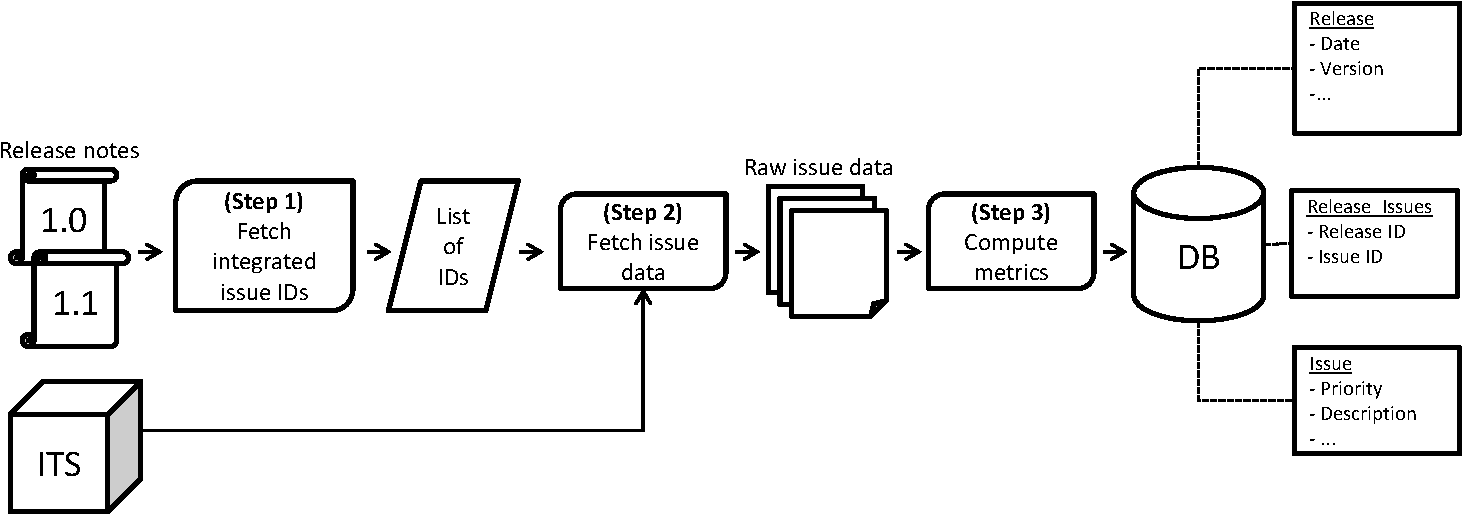
\includegraphics[width=\textwidth]{chapters/chapter4/figures/database_construction.pdf}
	\caption{\textbf{Data collection.} An overview of our approach to
	collect the needed data for studying delivery delay.}
	\label{ch4:fig:overview}
\end{figure} 

In Step 1, we consult the release notes of each studied project to identify the
release into which an addressed issue was \DIFdelbegin \DIFdel{integrated}\DIFdelend \DIFaddbegin \DIFadd{delivered}\DIFaddend . A release note is a
document that describes the content of a release. For instance, a release note
might provide information about the improvements that are included in a release (with
respect to prior releases), the new features, the fixed issues, and the known
problems. The Eclipse, ArgoUML, and Firefox projects publish their release notes on their
respective websites.\smartfoot{\url{https://www.mozilla.org/en-US/firefox/releases/}}

Unfortunately, release notes may not mention all of the fixed issues that have
been \DIFdelbegin \DIFdel{integrated into }\DIFdelend \DIFaddbegin \DIFadd{delivered through }\DIFaddend a release. This limitation hinders the possibility of
studying issues that were fixed but have not been \DIFdelbegin \DIFdel{integrated}\DIFdelend \DIFaddbegin \DIFadd{delivered}\DIFaddend , since we cannot
claim that an issue that is not listed in a release note was not \DIFdelbegin \DIFdel{integrated }\DIFdelend \DIFaddbegin \DIFadd{delivered }\DIFaddend (\eg
the development team may forget to list some \DIFdelbegin \DIFdel{integrated }\DIFdelend \DIFaddbegin \DIFadd{delivered }\DIFaddend fixed issues). However,
the fixed issues that are listed in a release note are more likely to have been
shipped to the end users (\ie it is unlikely that a release note would mention a fixed
issue that was not \DIFdelbegin \DIFdel{integrated}\DIFdelend \DIFaddbegin \DIFadd{delivered}\DIFaddend ). Hence, we choose to use release notes as a means
of linking fixed issues to releases in our database, despite the incompleteness
of such release notes---the release where we claim that an issue has been
\DIFdelbegin \DIFdel{integrated }\DIFdelend \DIFaddbegin \DIFadd{delivered }\DIFaddend is more likely to be correct (we elaborate more on this point in
\hyperref[ch4:threats]{Section}~\ref{ch4:threats}).

The output of Step 1 is a list of the issue IDs that have been fixed and
\DIFdelbegin \DIFdel{integrated}\DIFdelend \DIFaddbegin \DIFadd{delivered}\DIFaddend . To retrieve such a list for the Eclipse and Firefox projects, we
wrote a script to extract the listed issue IDs from all the release notes and
insert them into our database. The retrieved issue IDs are used to fetch the
issue report meta-data from the corresponding ITSs. In our database, we also
store the dates and version number of each release. 

\subsubsection*{\textbf{\textit{Step 2: Fetch issue data}}}

We use the collected issue IDs from Step~1 to retrieve information from their corresponding
issue reports, which
are recorded in the ITSs. Not all release notes of
the ArgoUML project
list the fixed issues of an official release. When they do,
only a few issues are listed (\eg
1-4).\smartfoot{\url{http://argouml.tigris.org/wiki/ReleaseSchedule/Past_Releases_in_Detail}}
To increase our sample of fixed issues for the ArgoUML project, we rely on its
ITS. We use the milestone field of
the issue reports to approximate the release into which an issue was \DIFdelbegin \DIFdel{integrated}\DIFdelend \DIFaddbegin \DIFadd{delivered}\DIFaddend .
Development milestones are counted towards the next official releases. For
instance, the development milestone
0.33.7\smartfoot{\url{http://argouml.tigris.org/issues/show_bug.cgi?id=4914}}
is counted towards the official release 0.34. The output of Step 2 is the raw
issue report data that is collected from ITSs.

Finally, to determine when an issue was fixed, we use the latest change to the
RESOLVED-FIXED status of that issue.  For instance, if an issue has its status
changed from RESOLVED-FIXED to REOPENED at $t_1$ and the status changes back to
RESOLVED-FIXED at $t_2$ (without changing again), we consider the corresponding
date of $t_2$ as the fix date. Also, we use the RESOLVED-FIXED status rather
than the VERIFIED-FIXED status, since we found that all of the issues that are
mapped to releases went through the RESOLVED-FIXED state before being \DIFdelbegin \DIFdel{integrated}\DIFdelend \DIFaddbegin \DIFadd{delivered}\DIFaddend , while
only a small percentage went through the VERIFIED-FIXED state. For example, only 17\% of
fixed issues in the Firefox project went through the VERIFIED-FIXED state.
We focus on issues that were resolved as RESOLVED-FIXED because they involve
changes to the source and/or test code that must be integrated into a release
before becoming visible to end users.

\subsubsection*{\textbf{\textit{Step 3: Compute metrics}}} \label{settings:step3}

After collecting the release date for each addressed issue, we compute all of the
attributes that may share a relationship with the types of delivery delay that
are presented in
\hyperref[ch2:deliverydelay]{Section}~\ref{ch2:deliverydelay}.

We first compute the delivery delay of addressed issues in terms of number of
releases (see~\hyperref[def:1]{Definition}~\ref{def:1}). We group this type of
delivery delay into four buckets: \textit{next}, \textit{after-1},
\textit{after-2}, and \textit{after-3-or-more}. The \textit{next} bucket
contains addressed issues that are \DIFdelbegin \DIFdel{integrated }\DIFdelend \DIFaddbegin \DIFadd{delivered }\DIFaddend immediately. The \textit{after-1},
\textit{after-2}, and \textit{after-3-or-more} buckets contain addressed issues
for which \DIFdelbegin \DIFdel{integration }\DIFdelend \DIFaddbegin \DIFadd{delivery }\DIFaddend is skipped by one, two, or three or more releases,
respectively.
\hyperref[ch4:fig:fixToIntegration]{Figure}~\ref{ch4:fig:fixToIntegration} shows
the distribution of the addressed issues among buckets for each studied project.
The ArgoUML project has the highest percentage of addressed issues that fall
into the \textit{next} bucket (66\%), whereas \textit{next} accounts for only
2\% and 38\% of addressed issues in the Firefox and Eclipse projects,
respectively. 

\begin{figure}
	\centering
	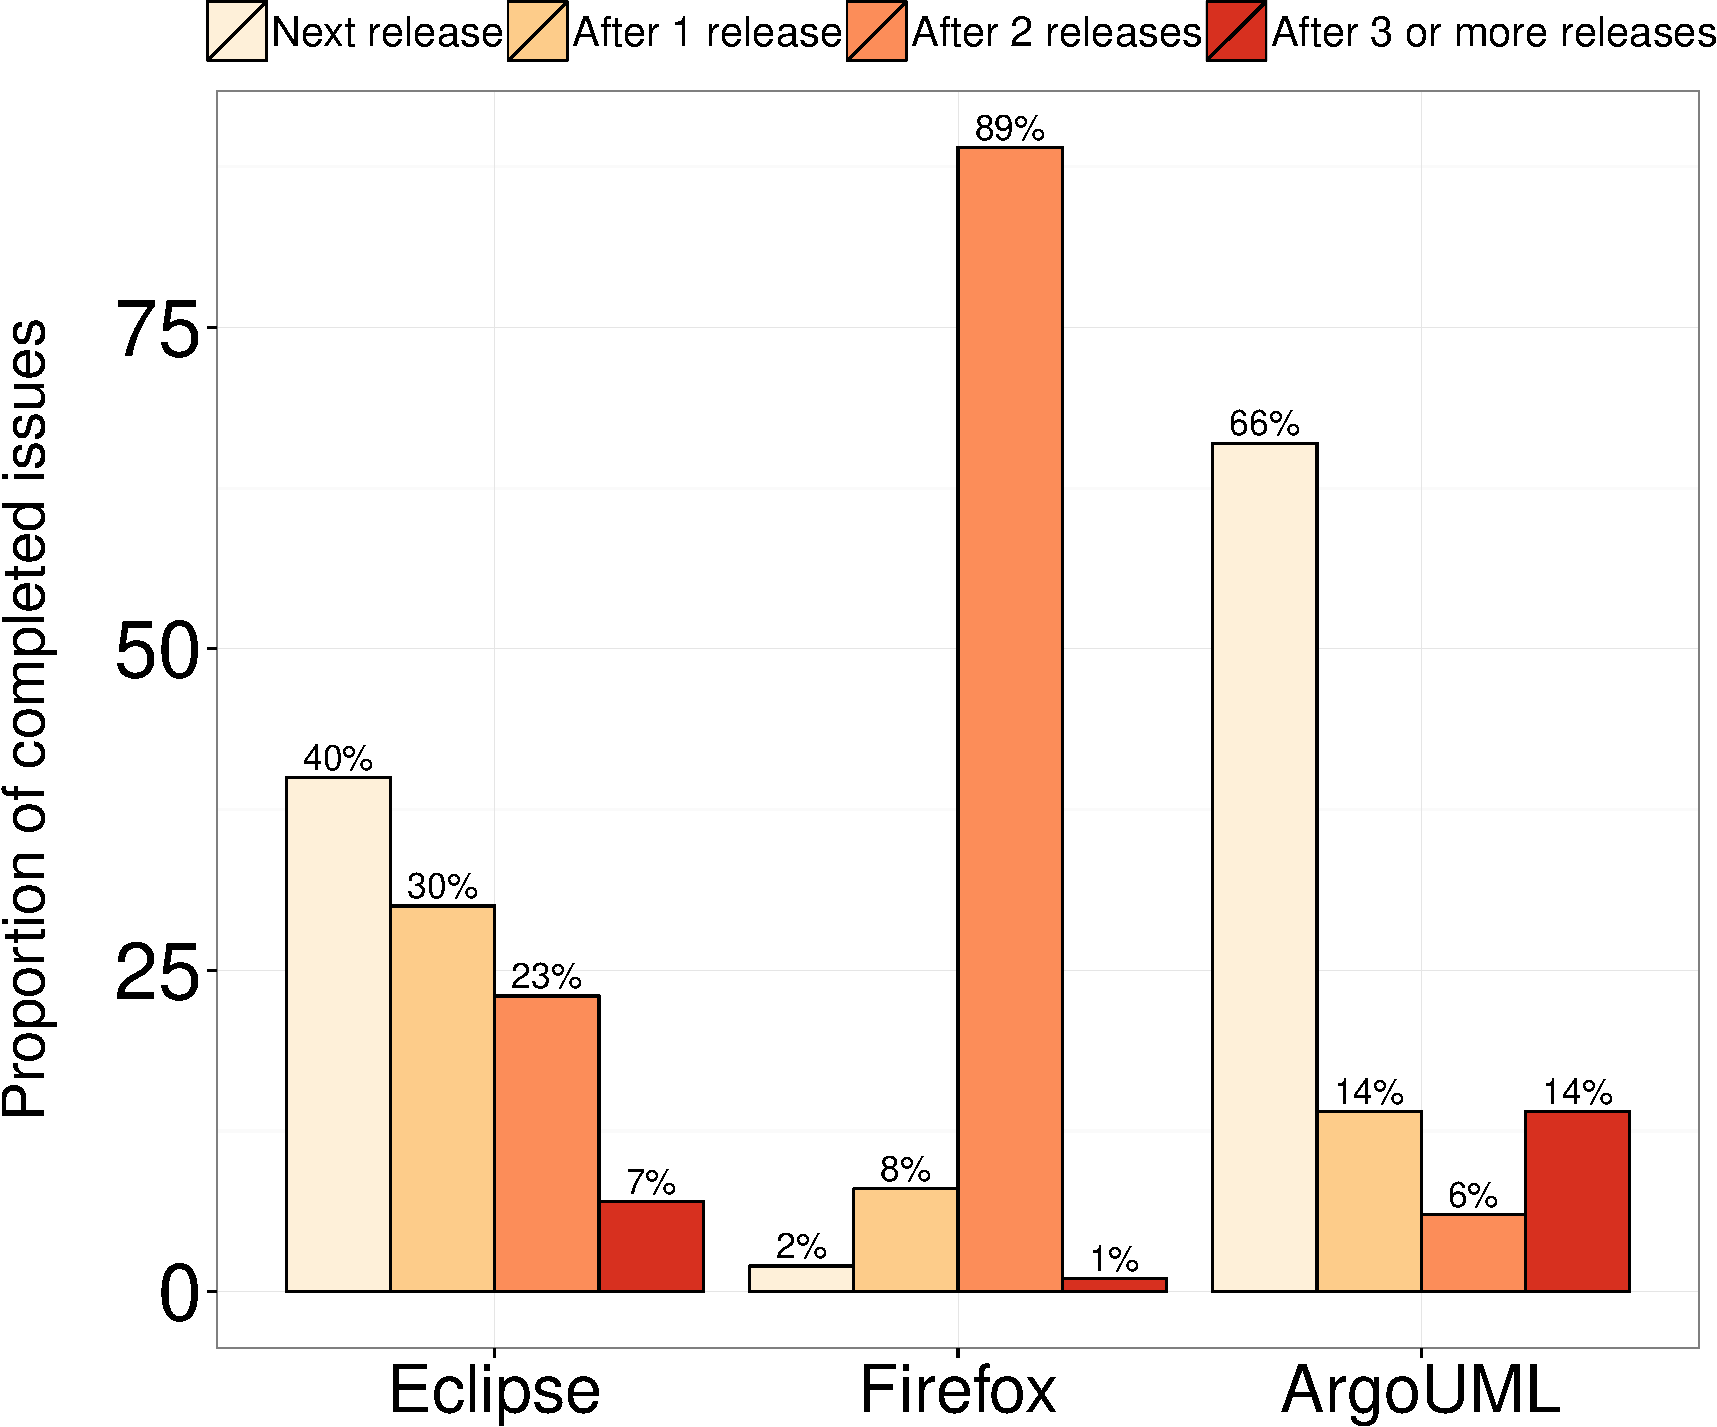
\includegraphics[width=0.7\textwidth]
	{chapters/chapter4/figures/CS_rq1-datasets.pdf}
	\caption{\textbf{Distribution of addressed issues per bucket.} The issues are
		grouped into \textit{next}, \textit{after-1}, \textit{after-2}, and
	\textit{after-3-or-more} buckets.}
	\label{ch4:fig:fixToIntegration}
\end{figure}

\begin{figure}
	\centering
	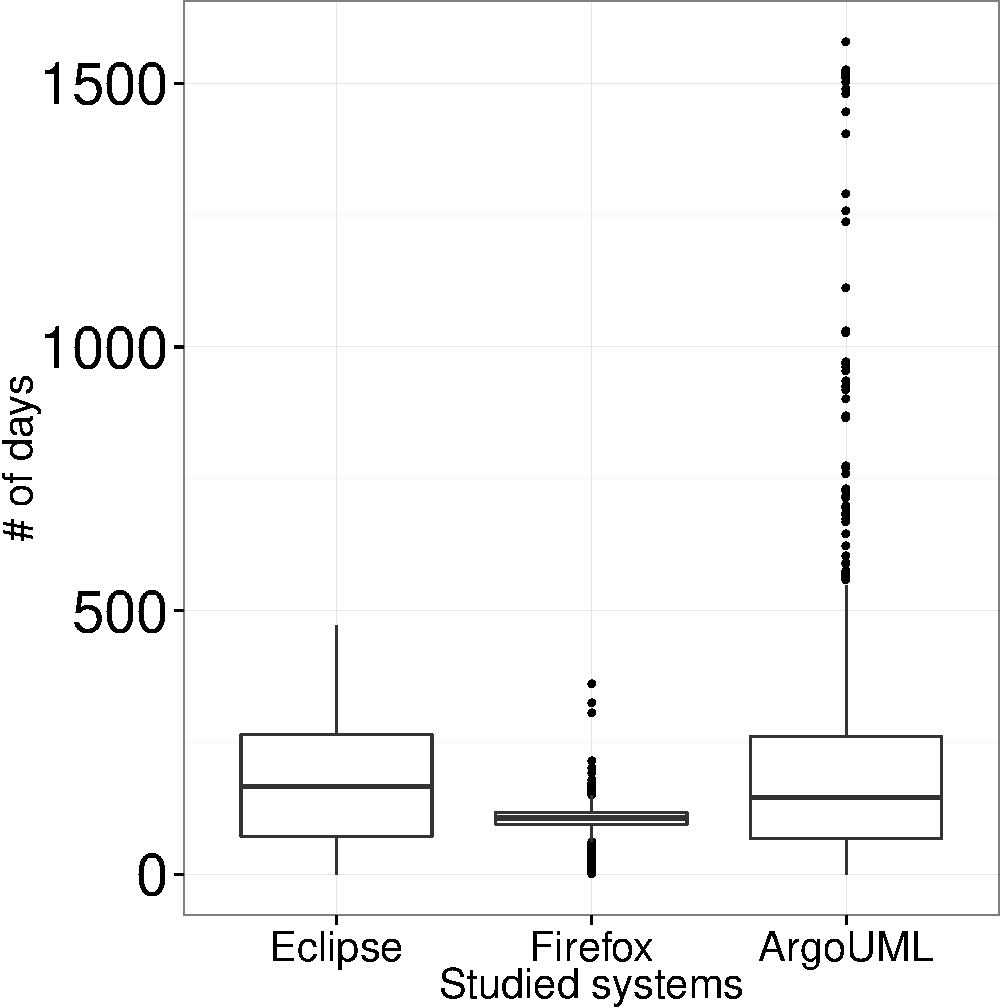
\includegraphics[width=0.60\textwidth,keepaspectratio]
	{chapters/chapter4/figures/boxplot-days-per-system.pdf}
	\caption{\textbf{Delivery delay in terms of days.} The medians 
		are 166, 107, and 146 days for the Eclipse, Firefox, and
		ArgoUML projects, respectively.
	}
	\label{ch4:fig:beanplot_days}
\end{figure}

Next, we compute the delivery delay in terms of number of days (see
\hyperref[def:2]{Definition}~\ref{def:2}).
\hyperref[ch4:fig:beanplot_days]{Figure}~\ref{ch4:fig:beanplot_days} shows the
distribution of delivery delay in terms of days for each studied project. The
Firefox project has the least skewed distribution of delivery delay. We use both
\hyperref[def:1]{Definitions}~\ref{def:1} and~\ref{def:2} of delivery delay to
address \hyperref[ch4:rq1]{RQ1}-\DIFdelbegin %DIFDELCMD < \hyperref[ch4:rq2]{RQ4}%%%
\DIFdelend \DIFaddbegin \hyperref[ch4:rq4]{RQ4}\DIFaddend .   

Finally, we identify issues that have a prolonged delivery delay in each studied
project (see \hyperref[def:3]{Definition}~\ref{def:3}). We group addressed
issues into \textit{prolonged delay} and \textit{normal delay} buckets.
Addressed issues, of which delivery delay is at least one MAD above the median
delivery delay of a subject project, fall into the \textit{prolonged delay}
bucket.  \hyperref[ch4:fig:beanplot_days]{Figure}~\ref{ch4:fig:beanplot_days}
shows that a prolonged delivery delay in one project may be a normal delivery
delay in another project (\eg the ArgoUML project {\em vs.} the Firefox
project). This figure highlights the importance of performing this analysis for
each project individually. We use this data to address \hyperref[ch4:rq5]{RQ5}
and \hyperref[ch4:rq6]{RQ6}.

We use exploratory models to study the relationship between attributes of
addressed issues (\eg severity and priority) and delivery delay. Our goal is to
understand which attributes are important for modeling the delivery delay of
addressed issues. \\

\section{Results} \label{ch3:results}

In this section, we present the motivation, approach, and results for each
investigated RQ. 

\subsection{RQ1: How often are addressed issues prevented
from being released?}\label{ch4:rq1}

\subsubsection*{RQ1: Motivation}

Users and contributors care most about the time for an addressed issue to become
available rather than the time duration to fix it. In this regard, it is
important to investigate whether addressed issues are being \DIFdelbegin \DIFdel{integrated }\DIFdelend \DIFaddbegin \DIFadd{delivered
}\DIFaddend immediately (\eg in the next possible release) or not, since a large delivery
delay may frustrate users. In \hyperref[ch:rq1]{RQ1}, we investigate how often
addressed issues are being prevented from \DIFdelbegin \DIFdel{integration}\DIFdelend \DIFaddbegin \DIFadd{delivery}\DIFaddend . The analysis of
\hyperref[ch:rq1]{RQ1} is our first step toward understanding how long is the
delivery delay of addressed issues.

\subsubsection*{RQ1: Approach} 

We compute the delivery delay of addressed issues in terms of number of releases
and number of days (as shown in \hyperref[def:1]{Definitions}~\ref{def:1}
and~\ref{def:2}). Next, we analyze if addressed issues are being prevented from
being released solely because their fix occurs in the end of their release
cycle. For instance, Rahman and Rigby~\cite{rahman2015release} observe a
rush-to-release in which many issues are addressed near the release date. For
each addressed issue, we compute the {\em fix timing} metric, which is the ratio
between (i) the remaining number of days---after an issue is addressed---for an
upcoming release over (ii) the duration in terms of days of its respective
release cycle (see
\hyperref[ch4:eq:fixtiming]{Equation}~\ref{ch4:eq:fixtiming}). The {\em fix
timing} values range from 0 to 1. A {\em fix timing} value close to 1 indicates
that an issue is addressed early in the release cycle, since the numerator and
denominator of \hyperref[ch4:eq:fixtiming]{Equation}~\ref{ch4:eq:fixtiming}
would be close to each other.

\begin{equation}
	\frac{\text{\# days that is remaining for a release}}{\text{release cycle duration}}
	\label{ch4:eq:fixtiming}
\end{equation}

\subsubsection*{RQ1: Results} \label{results:rq1}

\begin{figure}[!t]
	\centering
	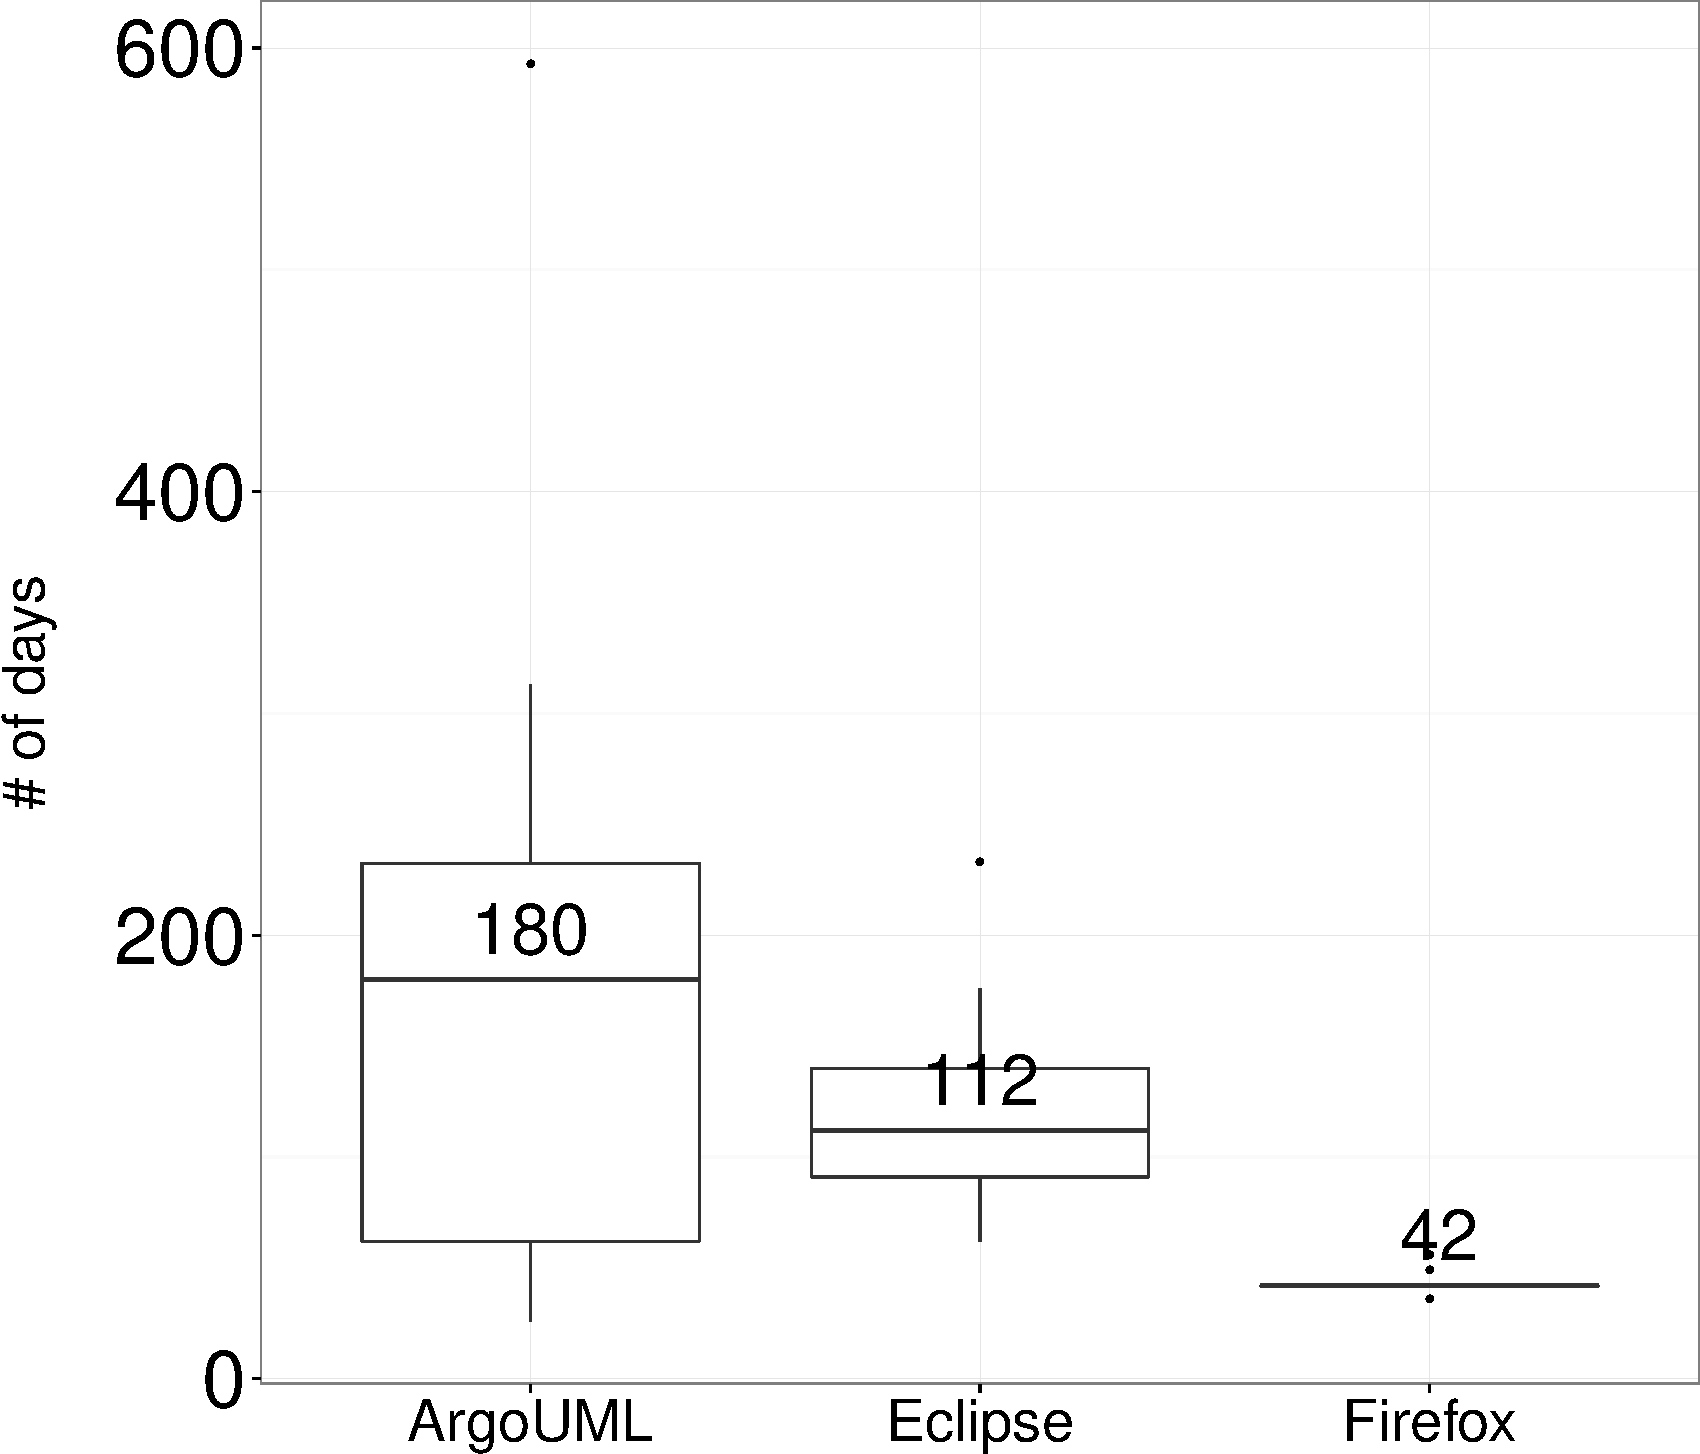
\includegraphics[width=0.7\textwidth]
	{chapters/chapter4/figures/RQ1_time_between_releases.pdf}
	\caption{\textbf{Number of days between the studied releases of the
	ArgoUML, Eclipse, and Firefox projects.} The number shown over each
boxplot is the median interval.}  
	\label{ch4:fig:releaseIntervals}
\end{figure}

\noindent\DIFdelbegin \textit{\textbf{\DIFdel{Addressed issues usually
miss the next release in the Firefox project.}}%DIFAUXCMD
}
%DIFAUXCMD
\DIFdelend \DIFaddbegin \finding{Addressed issues usually
miss the next release in the Firefox project.}{find1}
\DIFaddend \hyperref[ch4:fig:releaseIntervals]{Figure}~\ref{ch4:fig:releaseIntervals} shows the
difference between the studied projects in terms of the time interval between
their releases. The median time in days for the Firefox project (42 days) is
approximately $\frac{1}{4}$ that of the ArgoUML project (180 days), and
$\frac{1}{3}$ that of the Eclipse project (112 days). Unlike the Eclipse and
Firefox projects, the distribution for the ArgoUML project is skewed. In
addition, \hyperref[ch4:fig:fixToIntegration]{Figure}~\ref{ch4:fig:fixToIntegration}
shows that the vast majority of addressed issues for the Firefox project is
\DIFdelbegin \DIFdel{integrated
}\DIFdelend \DIFaddbegin \DIFadd{delivered
}\DIFaddend \textit{after-2} releases, whereas for the Eclipse and ArgoUML projects, the
majority is \DIFdelbegin \DIFdel{integrated }\DIFdelend \DIFaddbegin \DIFadd{delivered }\DIFaddend in the \textit{next} release. 

The reason for the difference may be due to the release policies that are
followed in each project. For example,
\hyperref[ch4:fig:releaseIntervals]{Figure}~\ref{ch4:fig:releaseIntervals} shows that
the Firefox project releases consistently every 42 days (six weeks), whereas the
time intervals between the releases of the ArgoUML project vary from 50 to 220
days. Indeed, the release guidelines for the ArgoUML project state that the
ArgoUML team should release at least one stable release every 8 months (see
\hyperref[argouml:releng]{Section}~\ref{argouml:releng}). The delivery
consistency of the Firefox releases might lead to addressed issues being prevented
from a greater number of releases, since the Firefox project rigidly adhere to a
six-week release schedule despite accumulating issues that could not be
\DIFdelbegin \DIFdel{integrated }\DIFdelend \DIFaddbegin \DIFadd{delivered }\DIFaddend (see \hyperref[firefox:releng]{Section}~\ref{firefox:releng}). 

Although an addressed issue usually misses the next release in the Firefox
project, issues are usually shipped faster when compared to the other projects.
Indeed, \hyperref[ch4:fig:beanplot_days]{Figure}~\ref{ch4:fig:beanplot_days} shows that
addressed issues in the Firefox project take a median of 107 days to be
released, while it takes 166 and 146 days in the Eclipse and ArgoUML projects,
respectively.\\

\noindent\DIFdelbegin \textit{\textbf{\DIFdel{34\% to 60\% of addressed issues had their integration
prevented from at least one release in the traditionally released projects.}}%DIFAUXCMD
}
%DIFAUXCMD
\DIFdelend \DIFaddbegin \finding{34\% to 60\% of addressed issues had their delivery
prevented from at least one release in the traditionally released
projects.}{find2}
\DIFaddend \hyperref[ch4:fig:fixToIntegration]{Figure}~\ref{ch4:fig:fixToIntegration} shows
that 98\% of the addressed issues in the Firefox project are prevented from
\DIFdelbegin \DIFdel{integration
}\DIFdelend \DIFaddbegin \DIFadd{delivery }\DIFaddend in at least one release. However, for the projects that adopt a more
traditional release cycle, \ie the ArgoUML and Eclipse projects, 34\% to 60\%
of the addressed issues are prevented from \DIFdelbegin \DIFdel{integration }\DIFdelend \DIFaddbegin \DIFadd{delivery }\DIFaddend in at least one release.
This result indicates that even though an issue is addressed, \DIFdelbegin \DIFdel{integration }\DIFdelend \DIFaddbegin \DIFadd{its delivery }\DIFaddend may be
prevented by one or more releases, which can frustrate end users.\\

\begin{figure}[!t]
	\centering
	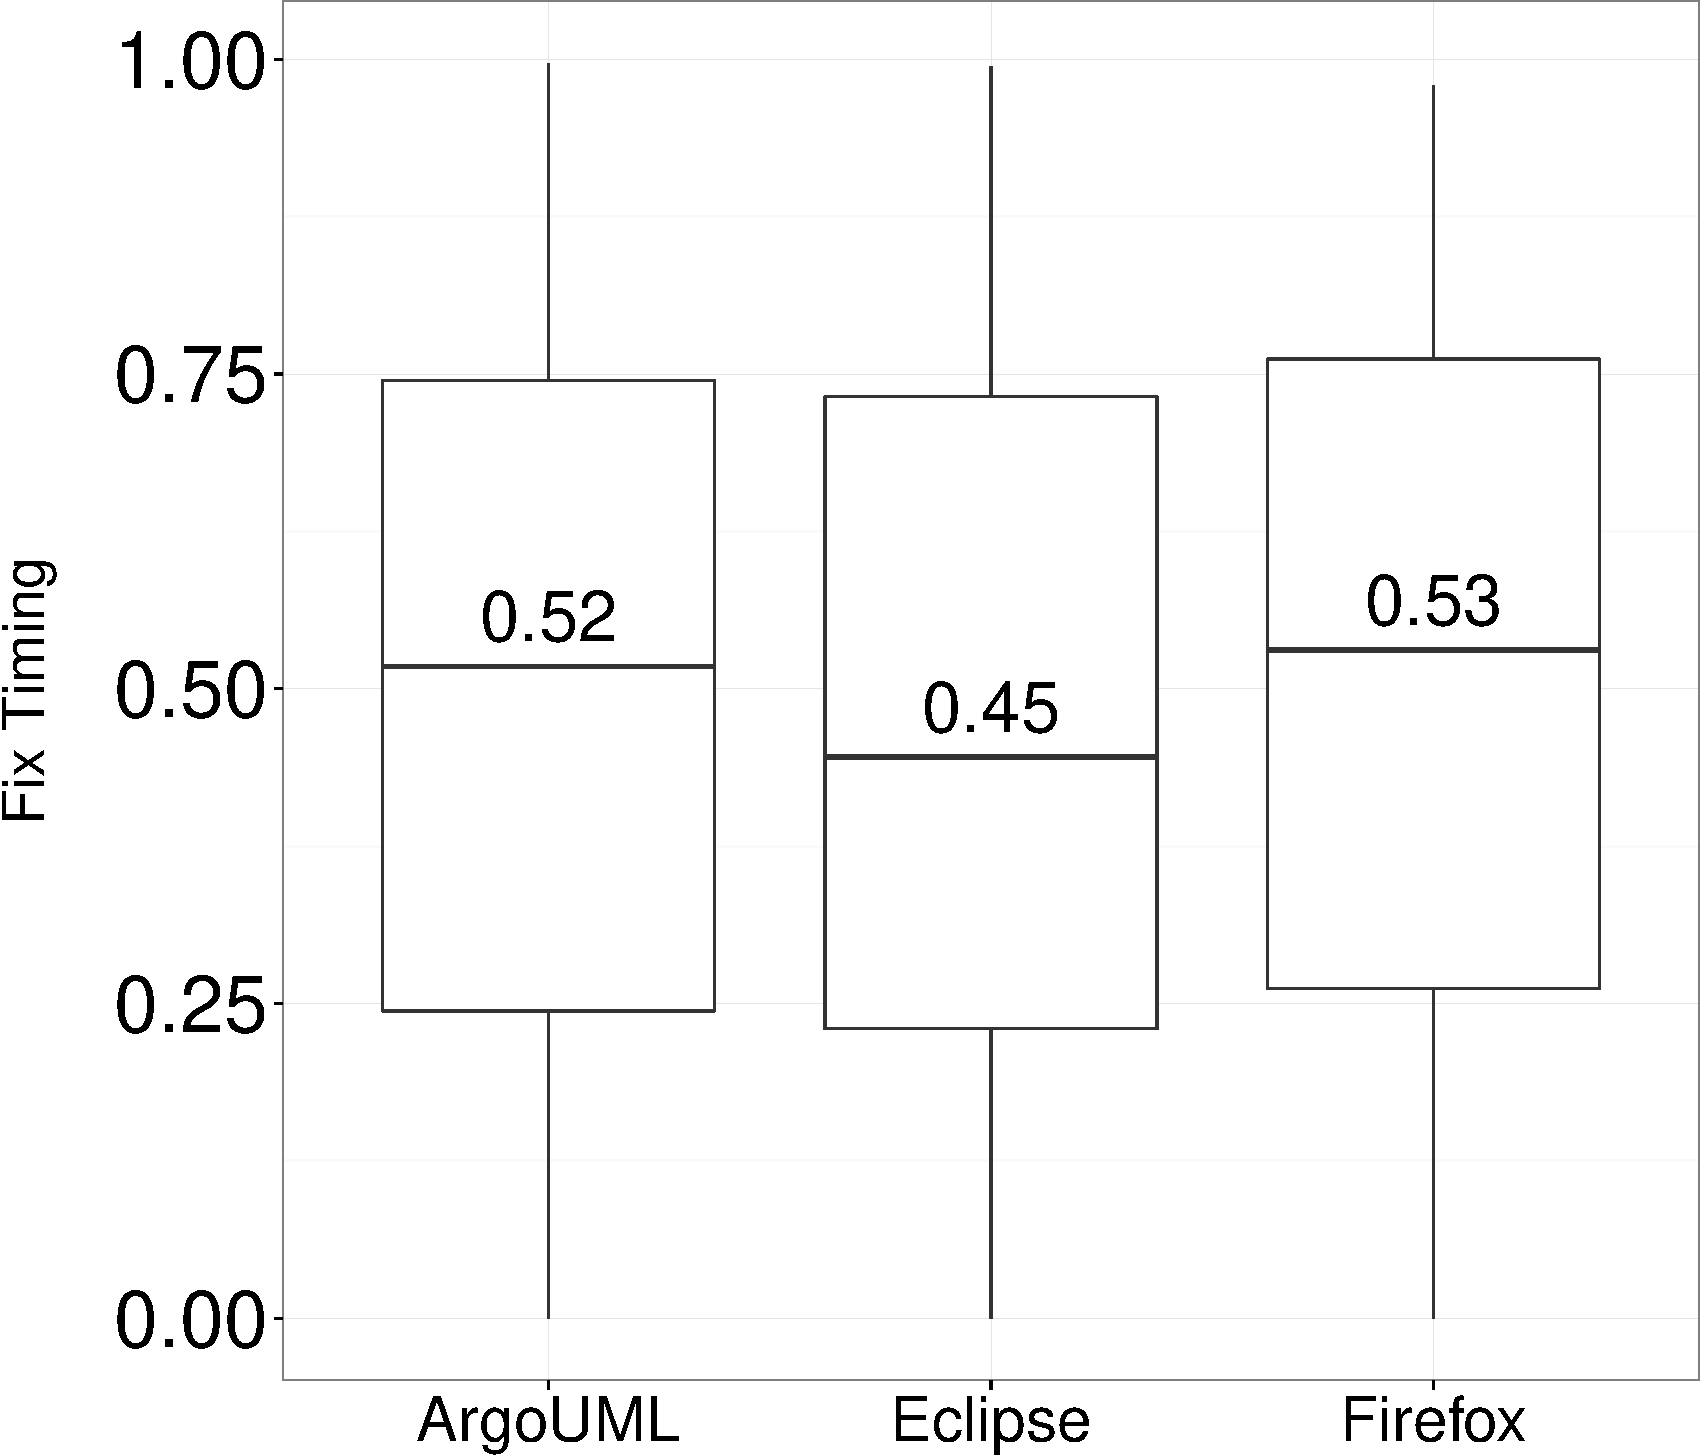
\includegraphics[width=0.7\textwidth]
	{chapters/chapter4/figures/addressing_stage.pdf}
	\caption{\textbf{Fix timing metric.} We present the
		distribution of the \textit{fix timing} metric for addressed
		issues that are prevented from \DIFdelbeginFL \DIFdelFL{integration }\DIFdelendFL \DIFaddbeginFL \DIFaddFL{delivery }\DIFaddendFL in at least one release.}
	\label{ch4:fig:boxplotTimeWindow}
\end{figure}

\noindent\DIFdelbegin \textit{\textbf{\DIFdel{Many issues that were prevented from integration are
addressed well before the upcoming release date.}}%DIFAUXCMD
} %DIFAUXCMD
\DIFdel{addressed }\DIFdelend \DIFaddbegin \finding{Many issues that were prevented from delivery are
addressed well before the upcoming release date.}{find3} \DIFadd{Addressed }\DIFaddend issues could be prevented
from \DIFdelbegin \DIFdel{integration }\DIFdelend \DIFaddbegin \DIFadd{delivery }\DIFaddend because they were addressed late in the release cycle, \eg one day
or one week before the upcoming release date. To check whether addressed issues are
being prevented from \DIFdelbegin \DIFdel{integration }\DIFdelend \DIFaddbegin \DIFadd{delivery }\DIFaddend mostly because they are being addressed late in the
release cycle, we compute the \textit{fix timing} metric. 

\hyperref[ch4:fig:boxplotTimeWindow]{Figure}~\ref{ch4:fig:boxplotTimeWindow} shows the
distribution of the \textit{fix timing} metric for each project. The smallest
\textit{fix timing} median is observed for the Eclipse project, which is 0.45.
For the ArgoUML and Firefox projects, the median is 0.52 and 0.53, respectively.
The \textit{fix timing} medians are roughly in the middle of the release.
Moreover, the boxes extend to cover between 0.25 and 0.75. The result suggests
that, in the studied projects, issues that are prevented from \DIFdelbegin \DIFdel{integration }\DIFdelend \DIFaddbegin \DIFadd{delivery }\DIFaddend are
usually addressed $\frac{1}{4}$ to $\frac{3}{4}$ of the way through a release.
Hence, it is unlikely that most addressed issues are prevented from \DIFdelbegin \DIFdel{integration
}\DIFdelend \DIFaddbegin \DIFadd{delivery
}\DIFaddend solely because they were addressed too close to an upcoming release date.

\DIFdelbegin %DIFDELCMD < \conclusionbox{The integration of 34\% to 60\% of the addressed issues in the
%DIFDELCMD < 	traditionally released projects and 98\% in the rapidly released project
%DIFDELCMD < 	were prevented from integration in at least one release. Furthermore, we
%DIFDELCMD < 	find that many issues which integration was prevented, were addressed well
%DIFDELCMD < before the releases from which they were omitted.}
%DIFDELCMD < %%%
\DIFdelend \DIFaddbegin \conclusionbox{The delivery of 34\% to 60\% of the addressed issues in the
	traditionally released projects and 98\% in the rapidly released project
	were prevented from delivery in at least one release. Furthermore, we
	find that many issues which delivery was prevented, were addressed well
before the releases from which they were omitted.}
\DIFaddend 


\subsection{RQ2: Does the stage of the release cycle impact
delivery delay?}\label{ch4:rq2}

\subsubsection*{RQ2: Motivation}

An issue that is {\em addressed} before the production of a {\em release candidate}
may receive more attention, which may lead to a shorter delivery delay.
Analysis of the impact of integration stage may help researchers and
practitioners to reflect on how to reduce delivery delay or to increase
awareness about it.

\subsubsection*{RQ2: Approach} 

For each studied project, we tag addressed issues according to the stage during
which they were addressed. For example, if an issue was addressed during the {\em beta}
stage of the Firefox project (\ie at the BETA channel), we tag such issue as
being ``{\em addressed during beta}''. We then compare the distributions of
delivery delay in terms of days (\hyperref[def:2]{Definition}~\ref{def:2})
among the different stages of a release cycle. For example, in the Firefox
project, we compare the distributions of delivery delay between the {\em
NIGHTLY}, {\em ALPHA}, and {\em BETA} stages, since the {\em RELEASE} stage
corresponds to the official release itself.

To check whether there is at least one statistically significant difference
among distributions of delivery delay, we use the Kruskal-Wallis
test~\cite{kruskal1952use}. This test checks if two or more samples are likely
to come from the same population ({\em null hypothesis}). However, when there are three or
more distributions, the Kruskal-Wallis test does not indicate which distribution
is statistically different with respect to the others. For specific comparisons
between distributions, we use the Dunn test~\cite{dunn1964multiple}. The Dunn
test shows which distribution is statistically different from the others. To
counteract the problem of multiple comparisons~\cite{dunn1961multiple}, we use
the Bonferroni correction to adjust our obtained $p$-$values$.

Finally, we use Cliff's delta to check the magnitude of the observed
differences~\cite{cliff1993dominance}. For example, two distributions may be
statistically different, but the magnitude of such a difference may be
negligible. The higher the value of the Cliff's delta, the greater the magnitude
of the difference between distributions. We use the thresholds provided by
Romano~\etal~\cite{romano_2006} to perform our comparisons: {\em delta} $<$
0.147 ({\em negligible}), {\em delta} $<$ 0.33 ({\em small}), {\em delta} $<$
0.474 ({\em medium}), and {\em delta} $>=$ 0.474 ({\em large}).

We also compute the {\em fix timing} metric (as in \hyperref[ch4:rq1]{RQ1}).
However, this time we check whether addressed issues are being prevented mostly
because they were performed near a code freeze date---rather than the upcoming
release date. \hyperref[ch4:eq:fixtiming2]{Equation}~\ref{ch4:eq:fixtiming2} shows how
we adapt \hyperref[ch4:eq:fixtiming]{Equation}~\ref{ch4:eq:fixtiming} to compute the
{\em fix timing} metric to account for the code freeze date. For the Eclipse
project, we consider the date of the last {\em release candidate} as the code
freeze stage, while we consider the date of a {\em beta stage} as the code
freeze stage in the ArgoUML project.

\begin{equation}
	\frac{\text{\# days that is remaining for a code freeze}}{\text{release
	cycle duration}}
	\label{ch4:eq:fixtiming2}
\end{equation}

\subsubsection*{RQ2: Results}

\noindent\DIFdelbegin \textit{\textbf{\DIFdel{Issues that are addressed during more stable stages of a
release cycle have a shorter delivery delay.}}%DIFAUXCMD
}
%DIFAUXCMD
\DIFdelend \DIFaddbegin \finding{Issues that are addressed during more stable stages of a
release cycle have a shorter delivery delay.}{find4}
\DIFaddend \hyperref[ch4:fig:cycle_phases]{Figure}~\ref{ch4:fig:cycle_phases} shows the
distributions of delivery delay (in terms of days) per each release cycle stage
of the studied projects. For the Eclipse project, the stages are divided into
{\em milestones}, {\em RCs} (Release Candidates), and {\em code freeze} (see the
\hyperref[eclipse:releng]{release engineering} process of Eclipse). Indeed,
issues that are addressed during RCs have a shorter delivery delay when compared
to issues that were addressed during milestone releases. For the difference
between {\em milestones} and {\em RCs}, we observe a $p=1.47 \times 10^{-52}$
and a {\em large} effect-size of $delta=0.63$. All of the $p$-$values$ and
$deltas$ of our statistical analysis are shown in
\hyperref[ch4:tbl:statisticalrq2]{Table}~\ref{ch4:tbl:statisticalrq2}. Even
though delivery delay seems to be larger during the {\em code freeze} stage, we
do not observe a significant $p$-$value$ when comparing the {\em code freeze}
stage \DIFdelbegin \DIFdel{to the other stages. }\DIFdelend \DIFaddbegin \DIFadd{with the }{\em \DIFadd{RC}} \DIFadd{stage. Additionally, although we obtain a $p=0.02$ when
comparing the }{\em \DIFadd{code freeze}} \DIFadd{stage with the }{\em \DIFadd{milestone}} \DIFadd{stage, we obtain
a }{\em \DIFadd{negligible}} \DIFadd{effect-size ($delta=0.09$), which indicates that the
difference of the values between distributions is not significant. }\DIFaddend In fact, only
ten issues were addressed during the {\em code freeze} stage in our data, which
impairs statistical observations of trends in such a stage.

For the Firefox project, we observe that delivery delay tends to be
shorter as fixes are performed along more stable stages. For example, by
comparing the delivery delay values between the {\em NIGHTLY} and {\em
AURORA} stages, we observe a $p=5.1 \times 10^{-49}$ and a {\em medium}
effect-size of $delta = 0.40$ (the other comparisons are shown in
\hyperref[ch4:tbl:statisticalrq2]{Table}~\ref{ch4:tbl:statisticalrq2}).

Finally, for the ArgoUML project, we also observe a trend of shorter
delivery delay as the fixes are performed during more stable stages of release
cycles. For instance, when we compare the delivery delay of addressed issues of the {\em alpha}
and {\em beta} stages, we obtain a $p$-$value$ of $3.98 \times 10^{-09}$ and a {\em
large} effect-size of $delta = 0.98$.\\

\begin{figure}
	\centering
	\DIFdelbeginFL %DIFDELCMD < \subfloat[Eclipse]{
%DIFDELCMD < 		\includegraphics[width=0.60\textwidth,keepaspectratio]
%DIFDELCMD < 		{chapters/chapter4/figures/eclipse_phases_boxplot.pdf}
%DIFDELCMD < 	}
%DIFDELCMD < %%%
\DIFdelendFL \DIFaddbeginFL \subfloat[Eclipse]{
		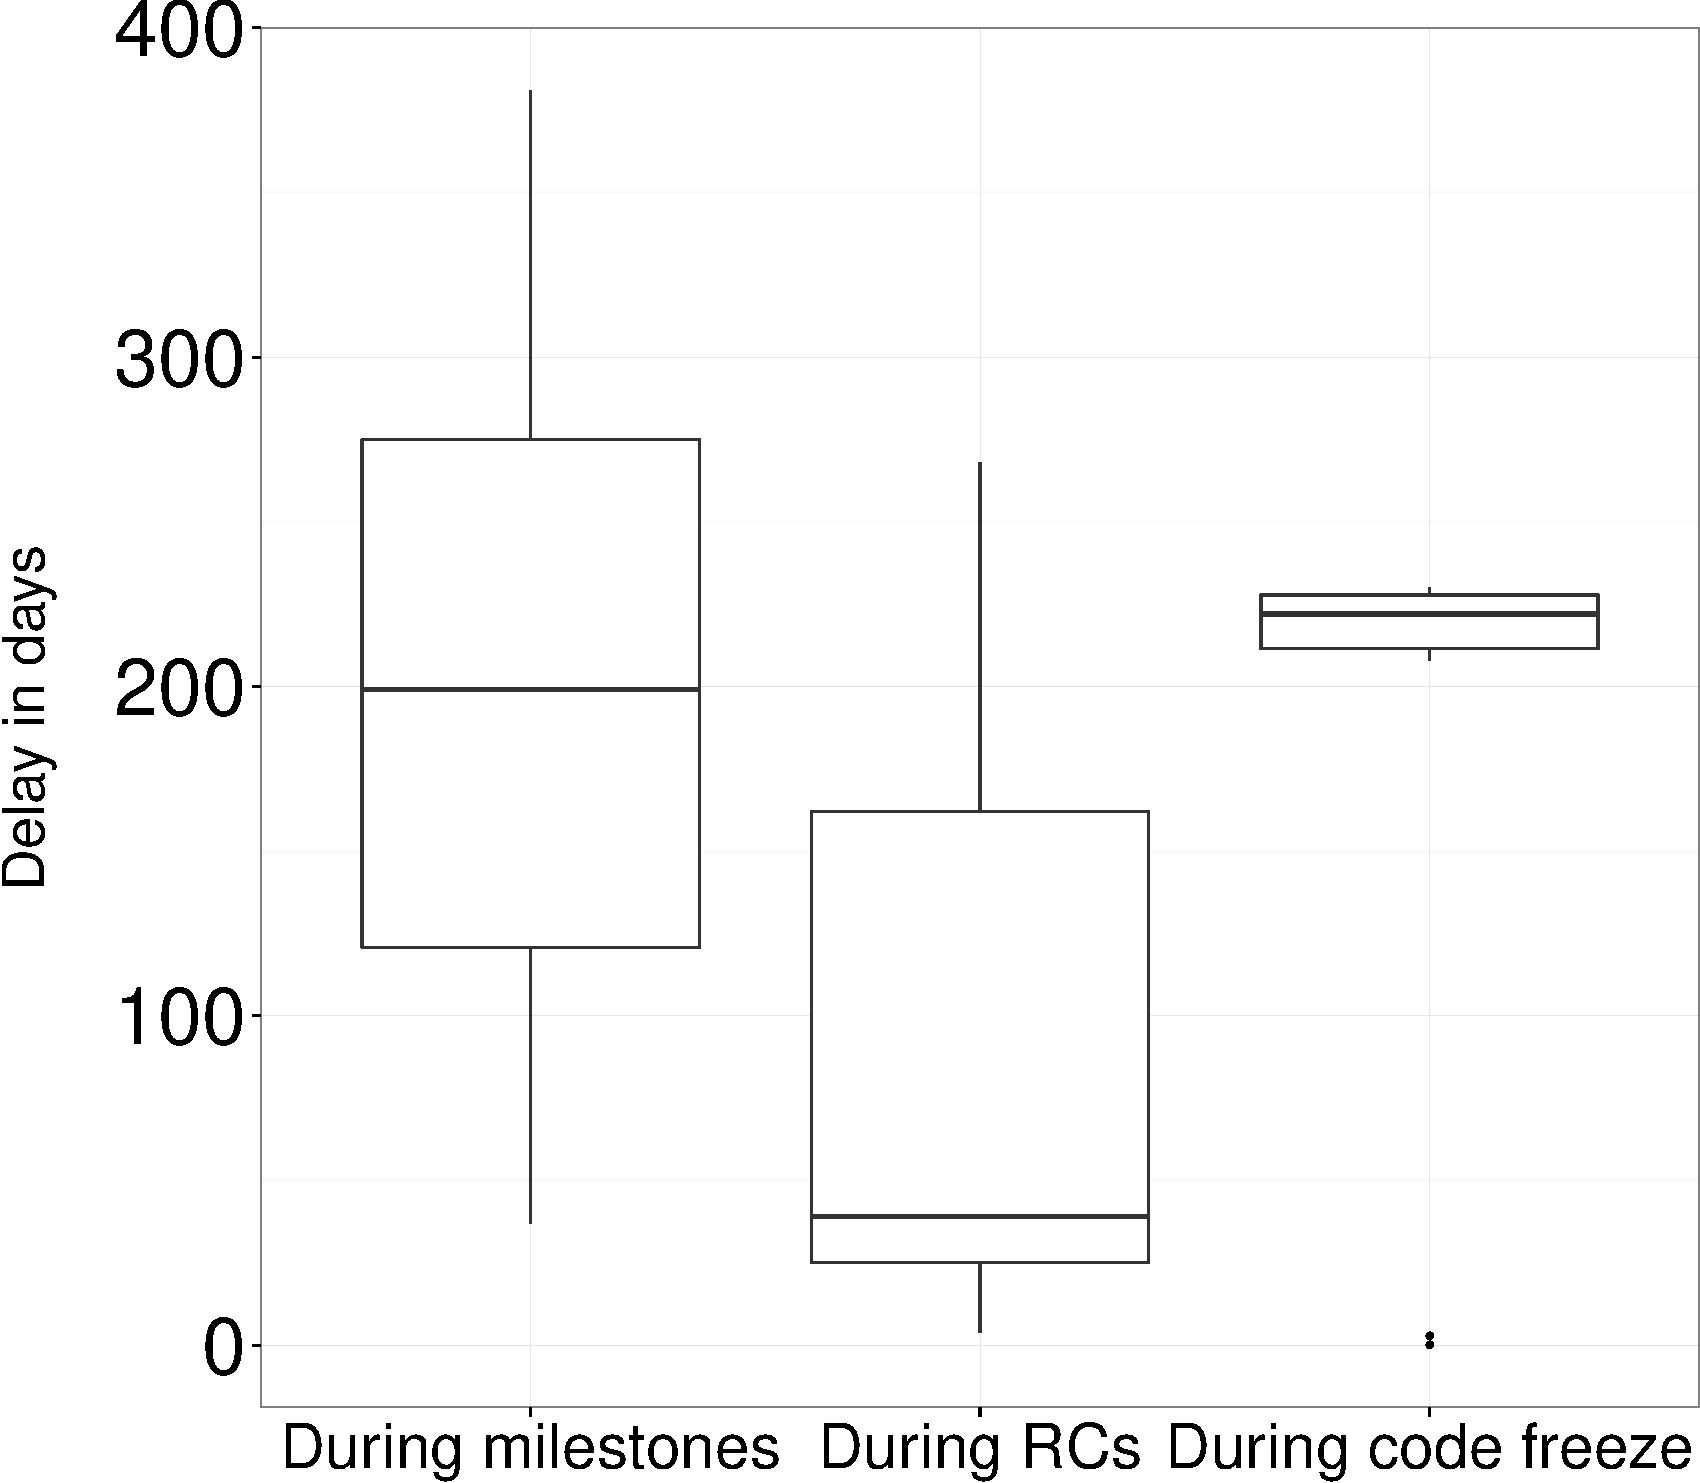
\includegraphics[width=0.50\textwidth,keepaspectratio]
		{chapters/chapter4/figures/eclipse_delay_per_stage.pdf}
	}
\DIFaddendFL 

	\DIFdelbeginFL %DIFDELCMD < \subfloat[Firefox]{
%DIFDELCMD < 		\includegraphics[width=0.60\textwidth,keepaspectratio]
%DIFDELCMD < 		{chapters/chapter4/figures/firefox_phases_boxplot.pdf}
%DIFDELCMD < 	}
%DIFDELCMD < %%%
\DIFdelendFL \DIFaddbeginFL \subfloat[Firefox]{
		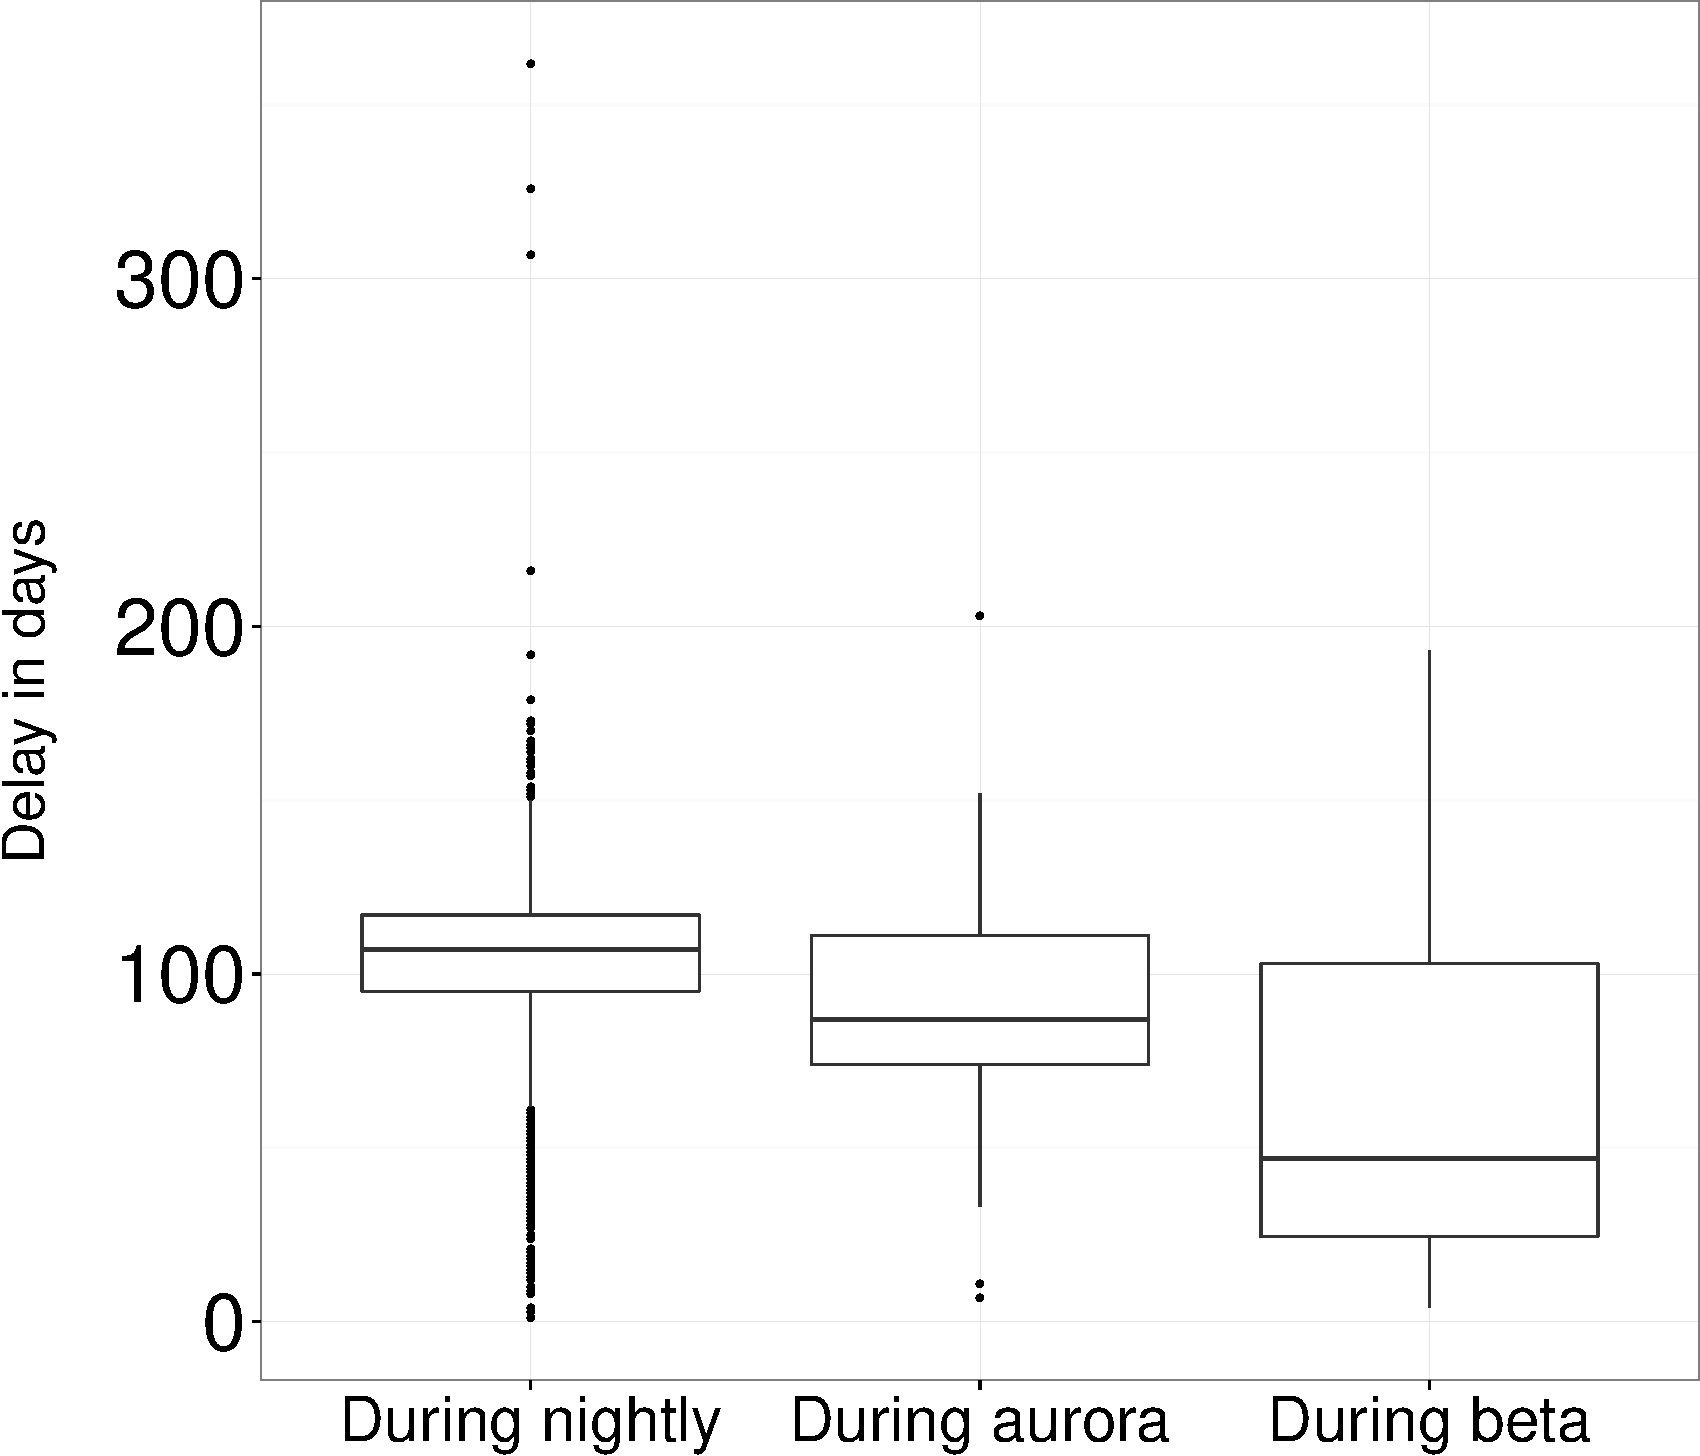
\includegraphics[width=0.50\textwidth,keepaspectratio]
		{chapters/chapter4/figures/firefox_delay_per_stage.pdf}
	}
\DIFaddendFL 

	\DIFdelbeginFL %DIFDELCMD < \subfloat[ArgoUML]{
%DIFDELCMD < 		\includegraphics[width=0.60\textwidth,keepaspectratio]
%DIFDELCMD < 		{chapters/chapter4/figures/argouml_phases_boxplot.pdf}
%DIFDELCMD < 	}
%DIFDELCMD < %%%
\DIFdelendFL \DIFaddbeginFL \subfloat[ArgoUML]{
		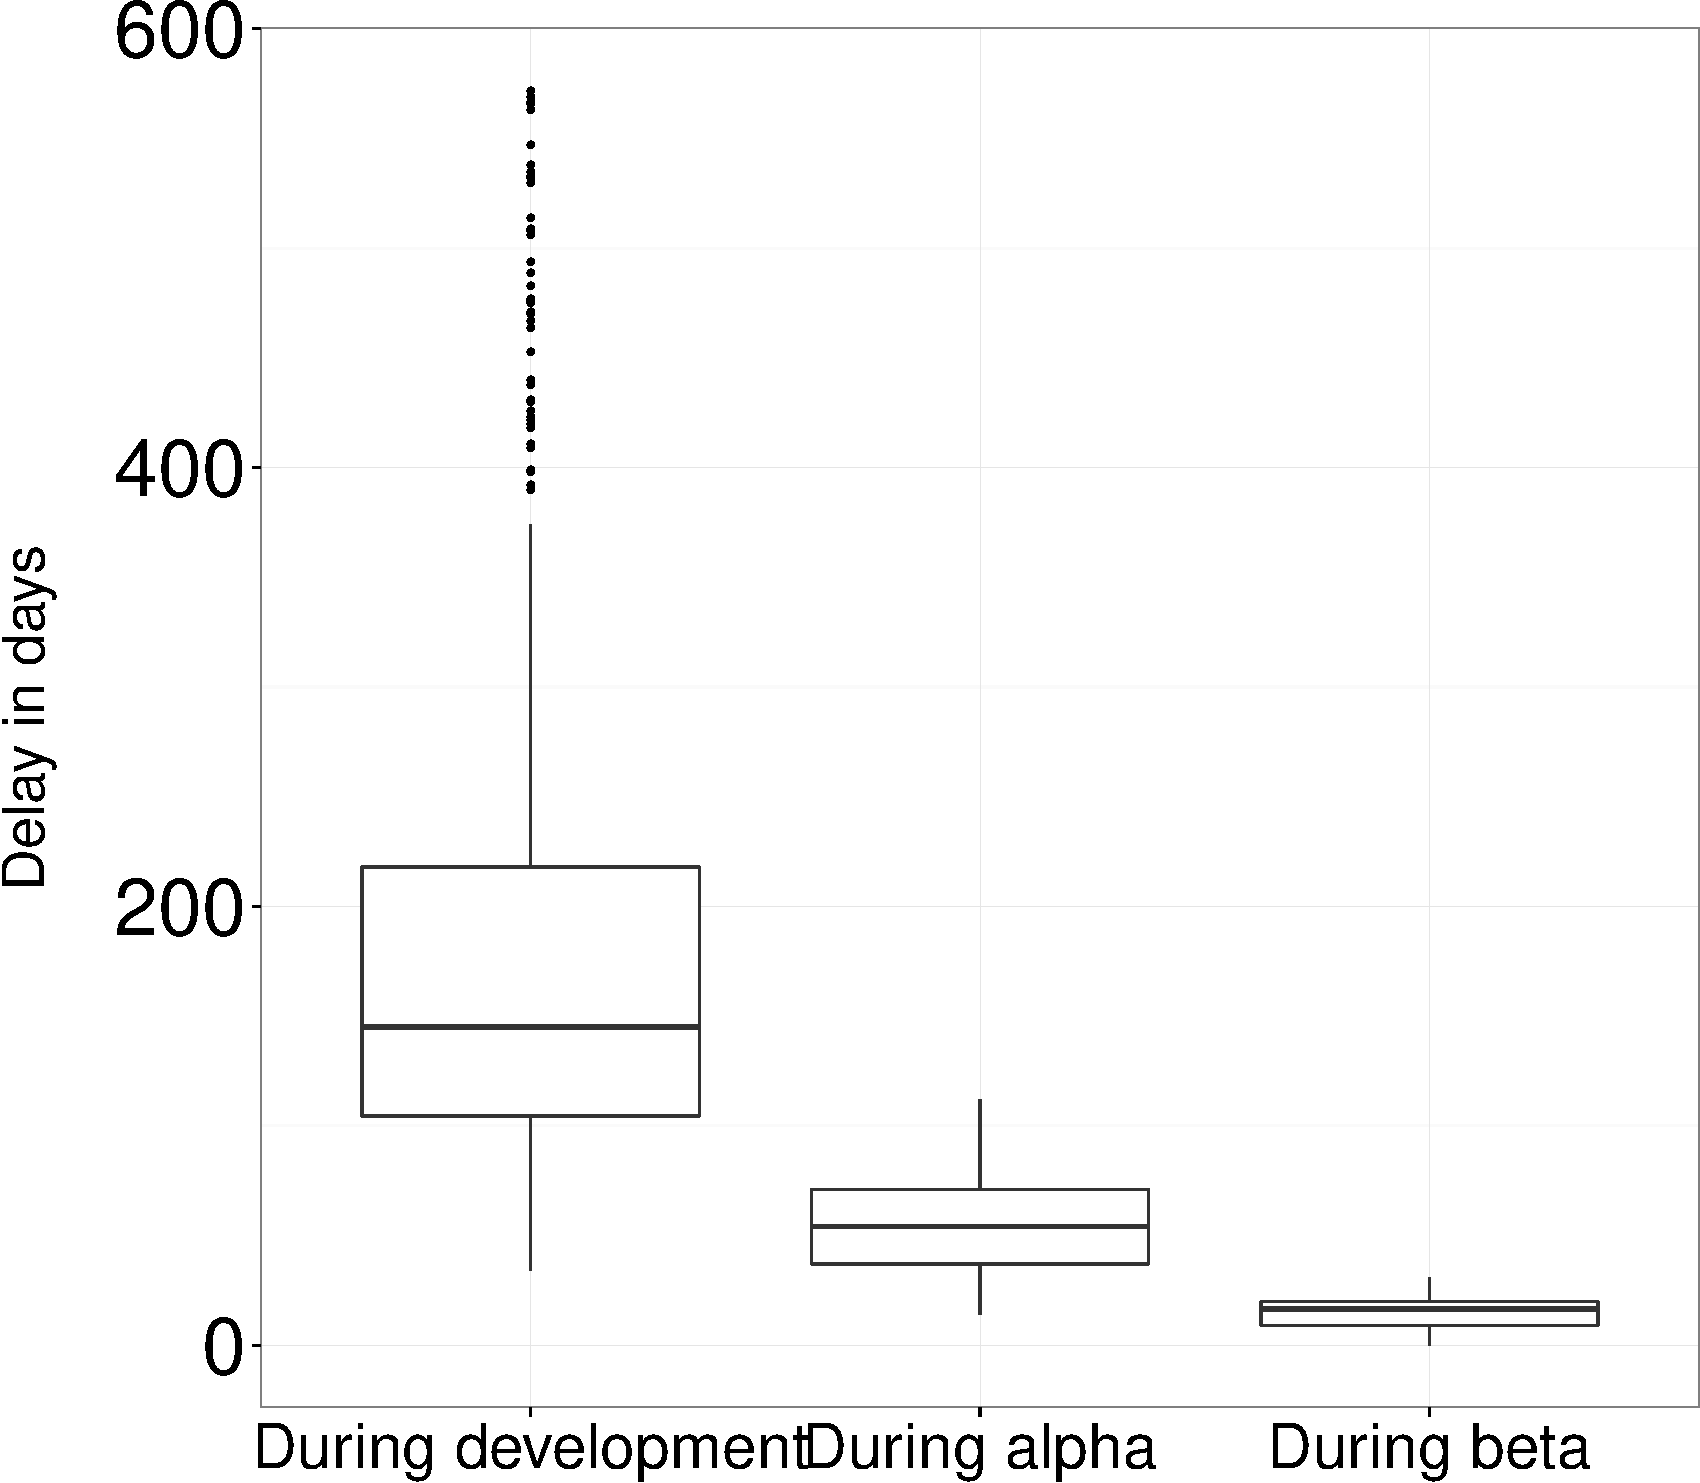
\includegraphics[width=0.50\textwidth,keepaspectratio]
		{chapters/chapter4/figures/argouml_delay_per_stage.pdf}
	}
\DIFaddendFL 

	\caption{\textbf{delivery delay during release
		cycle stages.} Issues that are addressed during more stable stages of a release cycle
	are likely to have a shorter delivery delay}
	\label{ch4:fig:cycle_phases}
\end{figure}


\begin{table}
	\footnotesize
	\centering
	\caption{\textbf{Statistical analysis.} An overview of the $p$-$values$
		and $deltas$ that are observed during our statistical analyses.
		\label{ch4:tbl:statisticalrq2}
	}
	\resizebox{\textwidth}{!}{
		\begin{tabular}{llrrr}
			\hline 
			& \textbf{Comparison} & \textbf{Kruskal-Wallis} ($p$) &
			\textbf{Dunn} ($p.adjusted$) & \textbf{Effect-size} ($delta$)\tabularnewline
			\hline 
			\multirow{3}{*}{\textbf{Eclipse}} & Milestones vs RCs &
			\multirow{3}{*}{$1.87 \times 10^{-51}$} & $1.47 \times 10^{-52}$ & (large) $0.63$\tabularnewline
			\cline{2-2} \cline{4-5} & RCs vs Code freeze &  & $0.56$ & Not apply\tabularnewline \cline{2-2} \cline{4-5} & Milestones vs Code freeze &  & $0.02$ & (negligible) $0.09$\tabularnewline
			\hline 
			\multirow{3}{*}{\textbf{Firefox}} & Nightly vs Aurora &
			\multirow{3}{*}{$2.99 \times 10^{-76}$} & $5.07 \times 10^{-49}$ &
			(medium) $0.40$\tabularnewline
			\cline{2-2} \cline{4-5} 
			& Aurora vs Beta &  & $1.72 \times 10^{-03}$ & (medium) $0.40$\tabularnewline
			\cline{2-2} \cline{4-5} 
			& Nightly vs Beta &  & $1.43 \times 10^{-31}$ & (large) $0.57$\tabularnewline
			\hline 
			\multirow{3}{*}{\textbf{ArgoUML}} & Development vs Alpha
			& \multirow{3}{*}{$2.73 \times 10^{-135}$} & $7.24 \times 10^{-89}$
			& (large) $0.94$\tabularnewline
			\cline{2-2} \cline{4-5} 
			& Alpha vs Beta &  & $3.98 \times 10^{-09}$ & (large) $0.98$\tabularnewline
			\cline{2-2} \cline{4-5} 
			& Development vs Beta &  & $1.14 \times 10^{-78}$ & (large) $0.99$\tabularnewline
			\hline 
		\end{tabular}
	}
\end{table}

\noindent\DIFdelbegin \textit{\textbf{\DIFdel{Many issues that are prevented from integration are
addressed well before the code freeze stage of their respective release cycle.}}%DIFAUXCMD
} %DIFAUXCMD
\DIFdelend \DIFaddbegin \finding{Many issues that are prevented from delivery are
addressed well before the code freeze stage of their respective release
cycle.}{find5} \DIFaddend We compute the {\em fix timing} metric that we present in
\hyperref[rq1]{RQ1}.  However, instead of counting the number of days until an
upcoming release, we count the number of days until an upcoming code freeze
stage (\hyperref[ch4:eq:fixtiming2]{Equation}~\ref{ch4:eq:fixtiming2}). Our goal
is to check whether addressed issues are being prevented from \DIFdelbegin \DIFdel{integration }\DIFdelend \DIFaddbegin \DIFadd{delivery }\DIFaddend mostly
because they are being addressed too close to a code freeze stage (\ie a period
during which integration of new code changes would likely be minimal).  

\begin{figure} \center 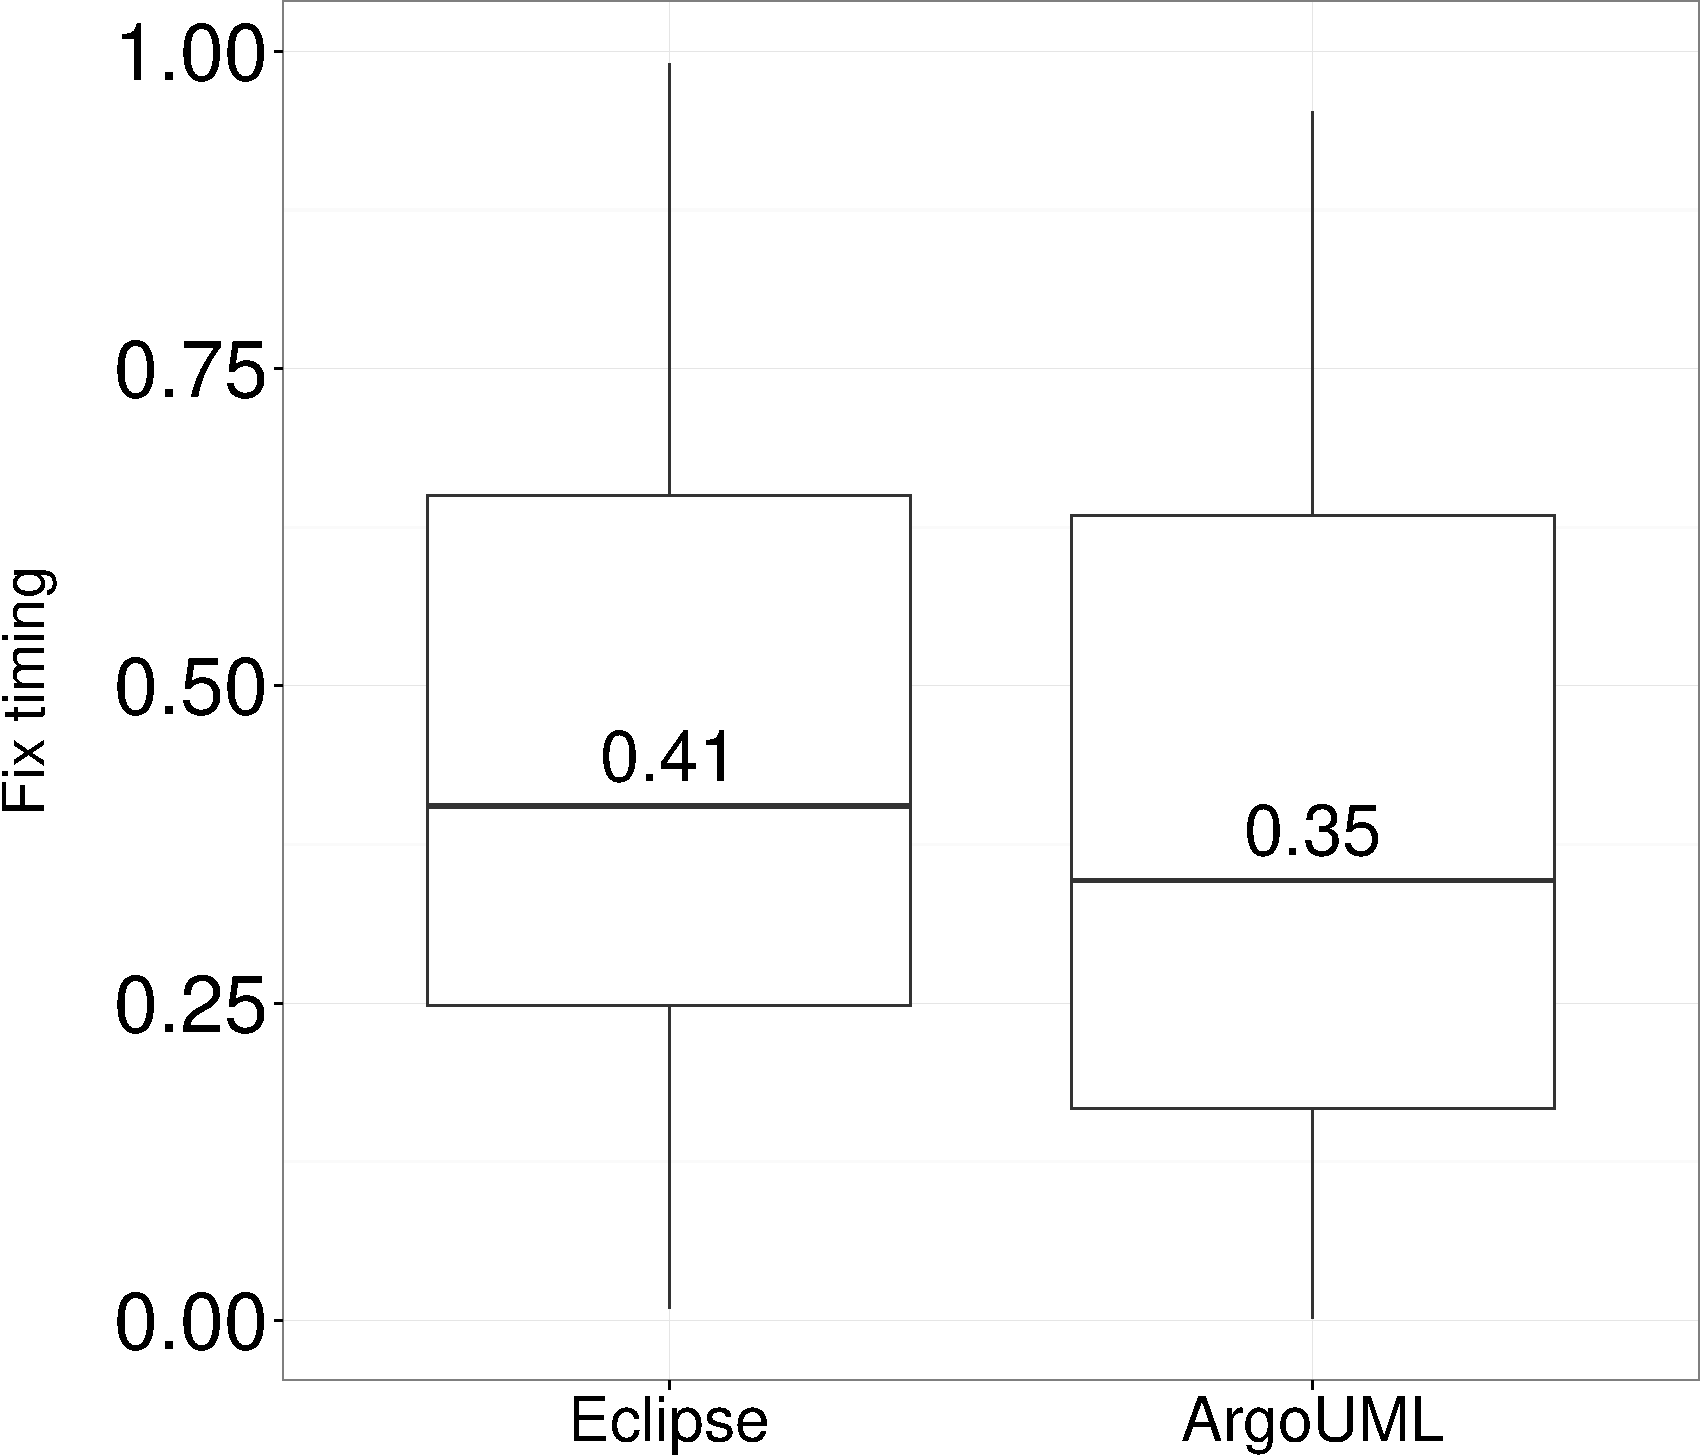
\includegraphics[width=0.60\textwidth,keepaspectratio]
	{chapters/chapter4/figures/as_codefreeze.pdf} \caption{\textbf{{\em Fix timing} values for
		the code freeze period.} The median {\em fix timing} values drop
		from 0.45 and 0.52 to 0.41 and 0.35 in the Eclipse and ArgoUML
projects, respectively. } \label{ch4:fig:codefreeze_allsystems} \end{figure}

In \hyperref[ch4:fig:codefreeze_allsystems]{Figure}~\ref{ch4:fig:codefreeze_allsystems},
we show the {\em fix timing} values for the Eclipse and ArgoUML projects, since
both projects adopt a {\em code freeze} stage. For the Eclipse project, the code
freeze starts after the last release candidate, while for the ArgoUML project,
the code freeze starts at the beginning of the {\em beta} stage (see
\hyperref[ch4:sec:subjects]{Section}~\ref{ch4:sec:subjects}). Naturally, we observe a
drop in the {\em fix timing} values, since both code freeze stages start considerably
before the official release dates. Nevertheless, we observe that even after correcting for
the code freeze stages of the Eclipse and ArgoUML projects, it is unlikely
that addressed issues are being prevented from \DIFdelbegin \DIFdel{integration }\DIFdelend \DIFaddbegin \DIFadd{delivery }\DIFaddend solely because of an approaching code
freeze stage. For instance, although the median {\em fix timing} for the ArgoUML project
dropped from 0.52 to 0.35, the development team would still have 2 months to
integrate an addressed issue---since the median duration of a release cycle in the
ArgoUML project is 180 days.

\DIFdelbegin %DIFDELCMD < \conclusionbox{We observe that issues that are addressed during more stable stages of
%DIFDELCMD < release cycles are associated with a shorter delivery delay. We also observe
%DIFDELCMD < that addressed issues are unlikely to be prevented from integration solely because
%DIFDELCMD < they were addressed near an upcoming code freeze stage.}
%DIFDELCMD < %%%
\DIFdelend \DIFaddbegin \conclusionbox{We observe that issues that are addressed during more stable stages of
release cycles are associated with a shorter delivery delay. We also observe
that addressed issues are unlikely to be prevented from delivery solely because
they were addressed near an upcoming code freeze stage.}
\DIFaddend 

\subsection{RQ3: How well can we model the delivery delay of
addressed issues?}\label{ch4:rq3}

\subsubsection*{RQ3: Motivation} 

Several studies have proposed approaches to investigate the time that is
required to fix an issue \cite{Anbalagan2009,Giger2010, Kim2006, Marks2011,
Weib2007, Zhang2013}. These studies could help to estimate when an issue will be
addressed. However, we find that an addressed issue may be prevented from
\DIFdelbegin \DIFdel{integration
}\DIFdelend \DIFaddbegin \DIFadd{delivery }\DIFaddend before reaching users. Even though most issues are addressed well before the next
release date, many of them are not \DIFdelbegin \DIFdel{integrated }\DIFdelend \DIFaddbegin \DIFadd{delivered }\DIFaddend until a future release. For users
and contributors, however, knowing the delivery delay of addressed issues is of
great interest. In \hyperref[ch4:rq3]{RQ3}, we investigate if we can accurately
model \DIFdelbegin \DIFdel{integration
time }\DIFdelend \DIFaddbegin \DIFadd{delivery delay }\DIFaddend in terms of number of releases and days (\ie
\hyperref[def:1]{Definitions}~\ref{def:1} and~\ref{def:2} of delivery delay).
Our explanatory models are important to understand which attributes may impact
delivery delay of addressed issues. Moreover, such type of models could be used by
practitioners to estimate when an addressed issue will likely be \DIFdelbegin \DIFdel{integrated}\DIFdelend \DIFaddbegin \DIFadd{delivered}\DIFaddend .

\begin{table}[t!]
	\caption{\textbf{Reporter, Resolver and Issue families.} Attributes of the
		Reporter, Resolver and Issue families that are used
		to model the delivery delay of addressed issues
		\label{ch4:tbl:dimensions}
	}
	\centering
	\footnotesize
	\begin{threeparttable}
		\begin{tabular}{rp{1.7cm}lp{9.6cm}}
			\hline
			\multicolumn{1}{c}{\textbf{Family}} &
			\multicolumn{1}{c}{\textbf{Attributes}} & \multicolumn{1}{c}{\textbf{Value}} &
			\multicolumn{1}{c}{\textbf{Definition (d)$\vert$Rationale (r)}}
			\\ \hline
			\multicolumn{ 1}{r}{\textbf{Reporter}} & Experience & Numeric & 
			\begin{tabular}{p{9.5cm}}
				\textbf{d:} Experience in filing reports for the
				project. It is measured by the number of previously
				reported issues of a reporter. \\ \hline \textbf{r:} An
				issue reported by an experienced reporter might be
				\DIFdelbeginFL \DIFdelFL{integrated }\DIFdelendFL \DIFaddbeginFL \DIFaddFL{delivered }\DIFaddendFL quickly.
			\end{tabular}
			\\ \cline{2-4}
			\multicolumn{ 1}{r}{} & Integration speed & Numeric &
			\begin{tabular}{p{9.5cm}}
				\textbf{d:} Measured by the median integration
				time of prior issues that were reported by a
				given reporter.\\ \hline
				\textbf{r:} If issues that are reported by a
				given reporter are \DIFdelbeginFL \DIFdelFL{integrated }\DIFdelendFL \DIFaddbeginFL \DIFaddFL{delivered }\DIFaddendFL quickly, future issues
				reported by the same reporter may also be
				\DIFdelbeginFL \DIFdelFL{integrated
				}\DIFdelendFL \DIFaddbeginFL \DIFaddFL{delivered }\DIFaddendFL quickly. 
			\end{tabular}
			\\ \hline
			\multicolumn{ 1}{r}{\textbf{Resolver}} &
			$^\dagger$Experience & Numeric & 
			\begin{tabular}{p{9.5cm}}
				\textbf{d:} Experience in fixing issues for the
				project. It is measured by the number 
				of prior issues that were addressed by a given resolver.
				\\ \hline \textbf{r:} An issue that is addressed by
				an experienced resolver may be easier to
				integrate.
			\end{tabular}
			\\ \cline{2-4}
			\multicolumn{ 1}{r}{} & $^\dagger$Integration speed & Numeric &
			\begin{tabular}{p{9.5cm}}
				\textbf{d:} Measured by the median integration
				time of prior addressed issues. \\ \hline
				\textbf{r:} If the prior addressed issues of a
				particular resolver were quickly \DIFdelbeginFL \DIFdelFL{integrated}\DIFdelendFL \DIFaddbeginFL \DIFaddFL{delivered}\DIFaddendFL ,
				future issues that are addressed by the same
				resolver may also be quickly \DIFdelbeginFL \DIFdelFL{integrated}\DIFdelendFL \DIFaddbeginFL \DIFaddFL{delivered}\DIFaddendFL . 
			\end{tabular}
			\\ \hline
			\multicolumn{ 1}{r}{\textbf{Issue}} & Component & Nominal &
			\begin{tabular}{p{9.5cm}}
				\textbf{d:} The component to which an issue is
				being reported. \\ \hline \textbf{r:} Issues that are
				related to a given component (\eg
				authentication) might be more important, and
				thus, might be \DIFdelbeginFL \DIFdelFL{integrated }\DIFdelendFL \DIFaddbeginFL \DIFaddFL{delivered }\DIFaddendFL more quickly than issues that are
				reported to less important components.
			\end{tabular}
			\\ \cline{ 2- 4}
			\multicolumn{ 1}{r}{} & Platform & Nominal & 
			\begin{tabular}{p{9.5cm}}
				\textbf{d:} The platform specified in the issue report.
				\\ \hline \textbf{r:} Issues regarding one platform
				(\eg MS Windows) might be \DIFdelbeginFL \DIFdelFL{integrated }\DIFdelendFL \DIFaddbeginFL \DIFaddFL{delivered }\DIFaddendFL more
				quickly than issues that are reported to
				less important platforms.
			\end{tabular}
			\\ \cline{ 2- 4}
			\multicolumn{ 1}{r}{} & Severity & Nominal &
			\begin{tabular}{p{9.5cm}}
				\textbf{d:} The severity level that
				is recorded in the issue report. \\ \hline
				\textbf{r:} severe issues (\eg
				blocking) might be \DIFdelbeginFL \DIFdelFL{integrated }\DIFdelendFL \DIFaddbeginFL \DIFaddFL{delivered }\DIFaddendFL faster than other issues.
				Panjer observed that the severity of an issue has a
				large effect on its lifetime for the Eclipse project
				\cite{Panjer2007}.
			\end{tabular}
			\\ \cline{ 2- 4}
			\multicolumn{ 1}{r}{} & Priority & Nominal &
			\begin{tabular}{p{9.5cm}}
				\textbf{d:} The priority that is assigned to the
				issue report. \\ \hline
				\textbf{r:} High priority issues will likely be
				\DIFdelbeginFL \DIFdelFL{integrated }\DIFdelendFL \DIFaddbeginFL \DIFaddFL{delivered }\DIFaddendFL before low priority issues. 
			\end{tabular}
			\\ \cline{2- 4}
			\multicolumn{ 1}{r}{} & $^\dagger$Stack trace attached & Boolean & 
			\begin{tabular}{p{9.5cm}}
				\textbf{d:} We check whether the issue report has a stack
				trace attached in its description. \\ \hline \textbf{r:}
				A stack trace attached in the description of the issue report may provide
				useful information with respect to the cause of the issue, which
				may quicken the \DIFdelbeginFL \DIFdelFL{integration }\DIFdelendFL \DIFaddbeginFL \DIFaddFL{delivery }\DIFaddendFL of that addressed issue
				\cite{schroter2010stack}.
			\end{tabular}
			\\ \cline{2-4}
			\multicolumn{ 1}{r}{} & Description Size & Numeric &
			\begin{tabular}{p{9.5cm}}
				\textbf{d:} Description of the issue measured by
				the number of words in its description. \\
				\hline \textbf{r:} Issues that are
				well-described might be easier to integrate than
				issues that are difficult to understand. 
			\end{tabular}
			\\ \hline
		\end{tabular}
		\begin{tablenotes}
		\item[$\dagger$] New attributes that did not appear in our
			previous work \cite{costa2014empirical}
		\end{tablenotes}
	\end{threeparttable}
\end{table}

\begin{table}[t!]
	\caption{\textbf{Project family.} Attributes of the
		Project family that is used
		to model the delivery delay of an addressed issue.
		\label{ch4:tbl:dimensions2}
	}
	\centering
	\footnotesize
	\begin{threeparttable}
		\begin{tabular}{rp{2.3cm}lp{9cm}}
			\hline
			\multicolumn{1}{c}{\textbf{Family}} &
			\multicolumn{1}{c}{\textbf{Attributes}} & \multicolumn{1}{c}{\textbf{Value}} &
			\multicolumn{1}{c}{\textbf{Definition (d)$\vert$Rationale (r)}}
			\\ \hline
			\multicolumn{ 1}{r}{\textbf{Project}} & Backlog of
			issues & Numeric &
			\begin{tabular}{p{8.9cm}}
				\textbf{d:} The number of issues in the RESOLVED-FIXED
				state at a given time. \\ \hline \textbf{r:} Having a
				large number of addressed issues at a given time might
				create a high workload on team members, which may affect
				the number of addressed issues that are \DIFdelbeginFL \DIFdelFL{integrated}\DIFdelendFL \DIFaddbeginFL \DIFaddFL{delivered}\DIFaddendFL .
			\end{tabular}
			\\ \cline{ 2- 4}
			\multicolumn{ 1}{r}{} & $^\dagger$Queue position  & Numeric & 
			\begin{tabular}{p{8.9cm}}
				\textbf{d:} $\frac{\text{rank of the
				issue}}{\text{all addressed issues}}$, where the
				rank is the position in time at which an issue
				was addressed in relation to others in the current
				release cycle. The rank is divided by all of the
				issues that were addressed until the end of the
				current release cyle. \\ \hline \textbf{r:} An
				issue that is near the front of the queue is
				more likely to be quickly \DIFdelbeginFL \DIFdelFL{integrated}\DIFdelendFL \DIFaddbeginFL \DIFaddFL{delivered}\DIFaddendFL .
			\end{tabular}                       
			\\ \hline
			\multicolumn{ 1}{r}{} & $^\dagger$Fixing time per
			resolver & Numeric & 
			\begin{tabular}{p{8.9cm}}
				\textbf{d:} $\frac{\sum\limits_{issue=1}^{total} \text{fixing
				time}}{\text{\# of resolvers}}$, the sum of the
				time (measured in terms of days)
				to fix the issues of the current release
				cycle over the number of resolvers that worked
				in that release cycle~\cite{mythical}. \\ \hline
				\textbf{r:} The higher the total fixing time
				that is spent per resolver in fixing issues the
				less the likelihood of an addressed issue
				experiencing a large delivery delay.
			\end{tabular}                       
			\\ \hline
			\multicolumn{ 1}{r}{} & $^\dagger$Backlog of issues per
			resolver& Numeric & 
			\begin{tabular}{p{8.9cm}}
				\textbf{d:} The number of issues in the
				RESOLVERD-FIXED state at a given time for each
				resolver of the development team. \\ \hline
				\textbf{r:} Having a large number of addressed
				issues per resolver might create a workload on
				that resolver to integrate the issue.
			\end{tabular}                       
			\\ \hline
		\end{tabular}
		\begin{tablenotes}
		\item[$\dagger$] New attributes that did not appear in our previous
			work \cite{costa2014empirical}
		\end{tablenotes}
	\end{threeparttable}
\end{table}

\begin{table}[t!]
	\caption{\textbf{Process family.} Attributes of the
		Process family that is used
		to model the delivery delay of an addressed issue.
		\label{ch4:tbl:dimensions3}
	}
	\centering
	\footnotesize
	\begin{threeparttable}
		\begin{tabular}{rp{2.3cm}lp{9cm}}
			\hline
			\multicolumn{1}{c}{\textbf{Family}} &
			\multicolumn{1}{c}{\textbf{Attributes}} & \multicolumn{1}{c}{\textbf{Value}} &
			\multicolumn{1}{c}{\textbf{Definition (d)$\vert$Rationale (r)}}
			\\ \hline
			\multicolumn{ 1}{r}{\textbf{Process}} & Number of Impacted Files & Numeric & 
			\begin{tabular}{p{8.9cm}}
				\textbf{d:} The number of files that are linked to an issue
				report. \\ \hline \textbf{r:} delivery delay
				might be related to a high number of impacted files
				because more effort would be required to properly
				integrate code modifications \cite{Jiang2013}. 
			\end{tabular}
			\\ \cline{ 2- 4}
			\multicolumn{ 1}{r}{} & Number of Activities & Numeric &
			\begin{tabular}{p{8.9cm}}
				\textbf{d:} An activity is an entry in the issue's
				history. \\ \hline \textbf{r:} A high number of
				activities might indicate that much work was necessary
				to fix the issue, which can impact the \DIFdelbeginFL \DIFdelFL{integration
				time }\DIFdelendFL \DIFaddbeginFL \DIFaddFL{delivery
				delay }\DIFaddendFL of an issue.~\cite{Jiang2013}. 
			\end{tabular}
			\\ \cline{ 2- 4}
			\multicolumn{ 1}{r}{} & Number of Comments & Numeric &
			\begin{tabular}{p{8.9cm}}
				\textbf{d:} The number of comments of an issue report.
				\\ \hline \textbf{r:} A large number of comments might
				indicate the importance of an issue or the difficulty
				to understand it~\cite{Giger2010}, which might impact
				delivery delay~\cite{Jiang2013}. 
			\end{tabular}
			\\ \cline{ 2- 4}
			\multicolumn{ 1}{r}{} & Number of Tosses & Numeric &
			\begin{tabular}{p{8.9cm}}
				\textbf{d:} The number of times that the issue's assignee has
				changed. \\ \hline \textbf{r:} The number of changes in
				the issue assignee might indicate a complex issue to
				fix or a difficulty in understanding such an issue,
				which can impact delivery delay. One of the
				reasons for changing the assigned developer is because
				additional expertise may be required to fix 
				an issue \cite{Jiang2013,Jeong2009}. 
			\end{tabular}
			\\ \cline{2-4}
			\multicolumn{ 1}{r}{} & Comment Interval & Numeric &
			\begin{tabular}{p{8.9cm}}
				\textbf{d:} The sum of all of the time intervals
				between comments (measured in hours) divided by the
				total number of comments. \\ \hline \textbf{r:} A short
				comment time interval indicates that an active
				discussion took place, which suggests that the issue is
				important.
				\cite{Jiang2013}. 
			\end{tabular}
			\\ \cline{2-4}
			\multicolumn{ 1}{r}{} & Churn & Numeric &
			\begin{tabular}{p{8.9cm}}
				\textbf{d:} The sum of the added lines and removed
				lines in the code repository. \\ \hline \textbf{r:} A
				higher churn suggests that a great amount of work was
				required to fix the issue, and hence, verifying the
				impact of integrating the modifications may also be
				difficult \cite{Nagappan2005, Jiang2013}.
			\end{tabular}
			\\ \cline{2-4}
			\multicolumn{ 1}{r}{} & $^\dagger$Fixing time & Numeric &
			\begin{tabular}{p{8.9cm}}
				\textbf{d:} The number of days between the
				moment at which an issue is opened the moment at
				which the issue is addressed (\ie the issue reaches
				the RESOLVED-FIXED status) \cite{Giger2010}. \\ \hline
				\textbf{r:} Issues that are addressed quickly might
				indicate that the necessary code changes are
				easy to integrate, wich may quicken \DIFdelbeginFL \DIFdelFL{integration
				time}\DIFdelendFL \DIFaddbeginFL \DIFaddFL{delivery delay}\DIFaddendFL . 
			\end{tabular}
			\\ \hline
		\end{tabular}
		\begin{tablenotes}
		\item[$\dagger$] New attributes that did not appear in our previous
			work \cite{costa2014empirical}
		\end{tablenotes}
	\end{threeparttable}
\end{table}

\subsubsection*{RQ3: Approach} 

In order to study when an addressed issue is \DIFdelbegin \DIFdel{integrated}\DIFdelend \DIFaddbegin \DIFadd{delivered}\DIFaddend , we collect information from
both the ITSs and VCSs of the studied systems. We train models using attributes
that are grouped in the following families: \textit{reporter},
\textit{resolver}, \textit{issue}, \textit{project}, and \textit{process}.
\begin{itemize}
	\item \textbf{Reporter:} refers to the attributes regarding an issue reporter.
		Issues that are reported by a reporter who is known to report important
		issues may receive more attention from the integration team.\\

	\item \textbf{Resolver:} refers to team members that fix issues.
		Issues that are addressed by experienced resolvers may be easier
		to integrate and ship to end users.\\

	\item \textbf{Issue:} refers to the attributes of issues reports. Project teams use this
		information to triage, fix, and integrate issues. For
		example, integrators may not be able to properly assess the
		importance and impact of poorly described issues, which may
		increase delivery delay.\\

	\item \textbf{Project:} refers to the status of the project when a
		specific issue is addressed. If the project team has a heavy
		integration workload, \ie many addressed issues waiting to be
		\DIFdelbegin \DIFdel{integrated, the integration }\DIFdelend \DIFaddbegin \DIFadd{delivered, the delivery }\DIFaddend of newly addressed issues \DIFdelbegin \DIFdel{are likely
		to have a longer delivery delay}\DIFdelend \DIFaddbegin \DIFadd{may be
		hindered}\DIFaddend .\\

	\item \textbf{Process:} refers to the process of fixing an issue. An
		addressed issue that involved a complex process (\eg long comment
		threads, large code changes) could be more difficult to
		understand and integrate.\\
\end{itemize}

\hyperref[ch4:tbl:dimensions]{Tables}~\ref{ch4:tbl:dimensions},
\ref{ch4:tbl:dimensions2} and~\ref{ch4:tbl:dimensions3} describe the attributes
that we compute for each family. For each attribute,
\hyperref[ch4:tbl:dimensions]{Tables}~\ref{ch4:tbl:dimensions},
\ref{ch4:tbl:dimensions2} and~\ref{ch4:tbl:dimensions3} present our rationale
for using it in our models. We choose these families of attributes because (i)
we intend to study a variety of perspectives that might influence delivery delay
and (ii) they are simple to compute using the publicly available data sources
(\eg ITSs and VCs) from our studied systems.

We train exploratory models to study how many releases an addressed issue is likely
to be prevented from \DIFdelbegin \DIFdel{integration }\DIFdelend \DIFaddbegin \DIFadd{delivery }\DIFaddend (\hyperref[def:1]{Definition}~\ref{def:1}). To
study delivery delay in terms of releases, we use the \textit{random forest}
classification technique \cite{RandomForest2001}. Random forest is an {\em
ensemble learning} technique that operates by combining a multitude of decision
trees at the training stage.  Each decision tree uses a random subset of the
attributes that are used to explain one phenomenon (\eg delivery delay). Next,
each decision tree votes for the response bucket (\eg {\em next} or {\em after-1}
release(s)) of a given instance. The majority of the votes for a given bucket
will be the actual response of the random forest. We choose random forests
because they are known to have a good overall accuracy and to be robust to
outliers as well as noisy data. Model robustness is important for our study
because the data in the ITSs tend to be noisy~\cite{Herraiz2008}. In our study,
we use the \textit{random forest} implementation provided by the \textit{bigrf}
R package.\smartfoot{Bigrf package \url{https://cran.r-project.org/src/contrib/Archive/bigrf/}} 

Since our data has a temporal order, \ie the values of the attributes for each
instance depends on the time at which the issue was addressed, we evaluate our
models by adapting the {\em Leave One Out Cross Validation} (LOOCV) technique.
In our LOOCV variation, we first sort the data by the date at which the issues
were addressed. Then, we train models to predict each next instance of the data. For
example, if issue $A$ is addressed before issue $B$, we train a model using $A$ and
test it using $B$. Furthermore, if issues $A$ and $B$ are addressed before $C$, we
train a model using $A$ and $B$ and test it using $C$. This process is repeated
until we test a model by using the last addressed issue in our data.

We evaluate the performance of our random forest models using the
\textit{precision}, \textit{recall}, \textit{F-measure}, and \textit{AUC}. We
also use \textit{Zero-R} models as a baseline to compare the results of our
models, since no prior models have been proposed to model delivery delay. We
describe each one below.

\textit{Precision} (P) measures the correctness of our models in estimating the
number of releases that are necessary to ship an addressed issue. An estimation is
considered correct if the estimated delivery delay is the same as the actual
delivery delay of an addressed issue. Precision is computed as the proportion of
correctly estimated delivery delay for each studied \DIFdelbegin \DIFdel{integration }\DIFdelend \DIFaddbegin \DIFadd{delivery delay }\DIFaddend bucket (\eg
next, after-1).

\textit{Recall} (R) measures the completeness of a model. A model is considered
complete if all of the addressed issues that were \DIFdelbegin \DIFdel{integrated }\DIFdelend \DIFaddbegin \DIFadd{delivered }\DIFaddend in a given release
\(r\) are estimated to appear in \(r\).  Recall is computed as the proportion of
issues that actually appear in a release \(r\) that were correctly estimated as
such.

\textit{F-measure} (F) is the harmonic mean of precision and recall, (\ie $\frac
{2 \times P \times R}{P + R}$). F-measure combines the inversely related
precision and recall values into a single descriptive statistic. 

\textit{Area Under the Curve} (AUC) is used to evaluate the degree of
discrimination achieved by the model \cite{hanley1982meaning}. For instance, AUC
can be used to evaluate how well our models can distinguish between addressed issues
that are prevented from \DIFdelbegin \DIFdel{integration }\DIFdelend \DIFaddbegin \DIFadd{delivery }\DIFaddend into one or two releases. The AUC is the
area below the curve plotting the true positive rate against false positive
rate. The value of AUC ranges between 0 (worst) and 1 (best). An area greater
than 0.5 indicates that the explanatory model outperforms a random predictor. We
computed the AUC value for a given bucket \(b\) (\eg \textit{next}) on a binary
basis. In other words, the probabilities of the instances were analyzed as
pertaining to a given bucket \(b\) or not. For example, when computing the AUC
value for the \textit{next} bucket, the AUC value is computed by verifying if an
instance belongs to the \textit{next} bucket or not. This process is repeated
for each bucket. Therefore, each bucket has its own AUC value.  

\textit{Zero-R models} are na\"{i}ve models that always select the bucket with
the highest number of instances. For example, a Zero-R model trained with the
Firefox project data would always select \textit{after-2} as the response for
each instance. 

We also study the delivery delay in terms of number of days
(\hyperref[def:2]{Definition}~\ref{def:2}). We train linear regression models
(using the \textit{ordinary least squares} technique~\cite{springertexts}) to
study delivery delay in terms of days. Linear regression is an approach for
modeling relationships between a dependent variable $y$ and one or more
explanatory variables $x$. When a single explanatory variable is used, the
approach is called {\em simple linear regression}, whereas when several
explanatory variables are used, the approach is called {\em multiple linear
regression}~\cite{freedman2009statistical}.  Regression models fit a curve of
the form $y = \beta_0 + \beta_{1}X_1 + \beta_{2}X_2 + ... + \beta_{n}X_n$. The
$y$ variable is the response variable (\ie delivery delay in terms of days in
our case), while the set of ${X}$ variables represent explanatory variables that
may share a relationship with $y$. The set of $\boldsymbol{\beta}$ coefficients
represent weights given by the model to adjust the values of $X$ to better
estimate the response $y$. The set of explanatory variables that we use in our
study are the attributes that are outlined in
\hyperref[ch4:tbl:dimensions]{Tables}~\ref{ch4:tbl:dimensions},~\ref{ch4:tbl:dimensions2}~and~\ref{ch4:tbl:dimensions3}.  

\begin{figure}
	\centering
	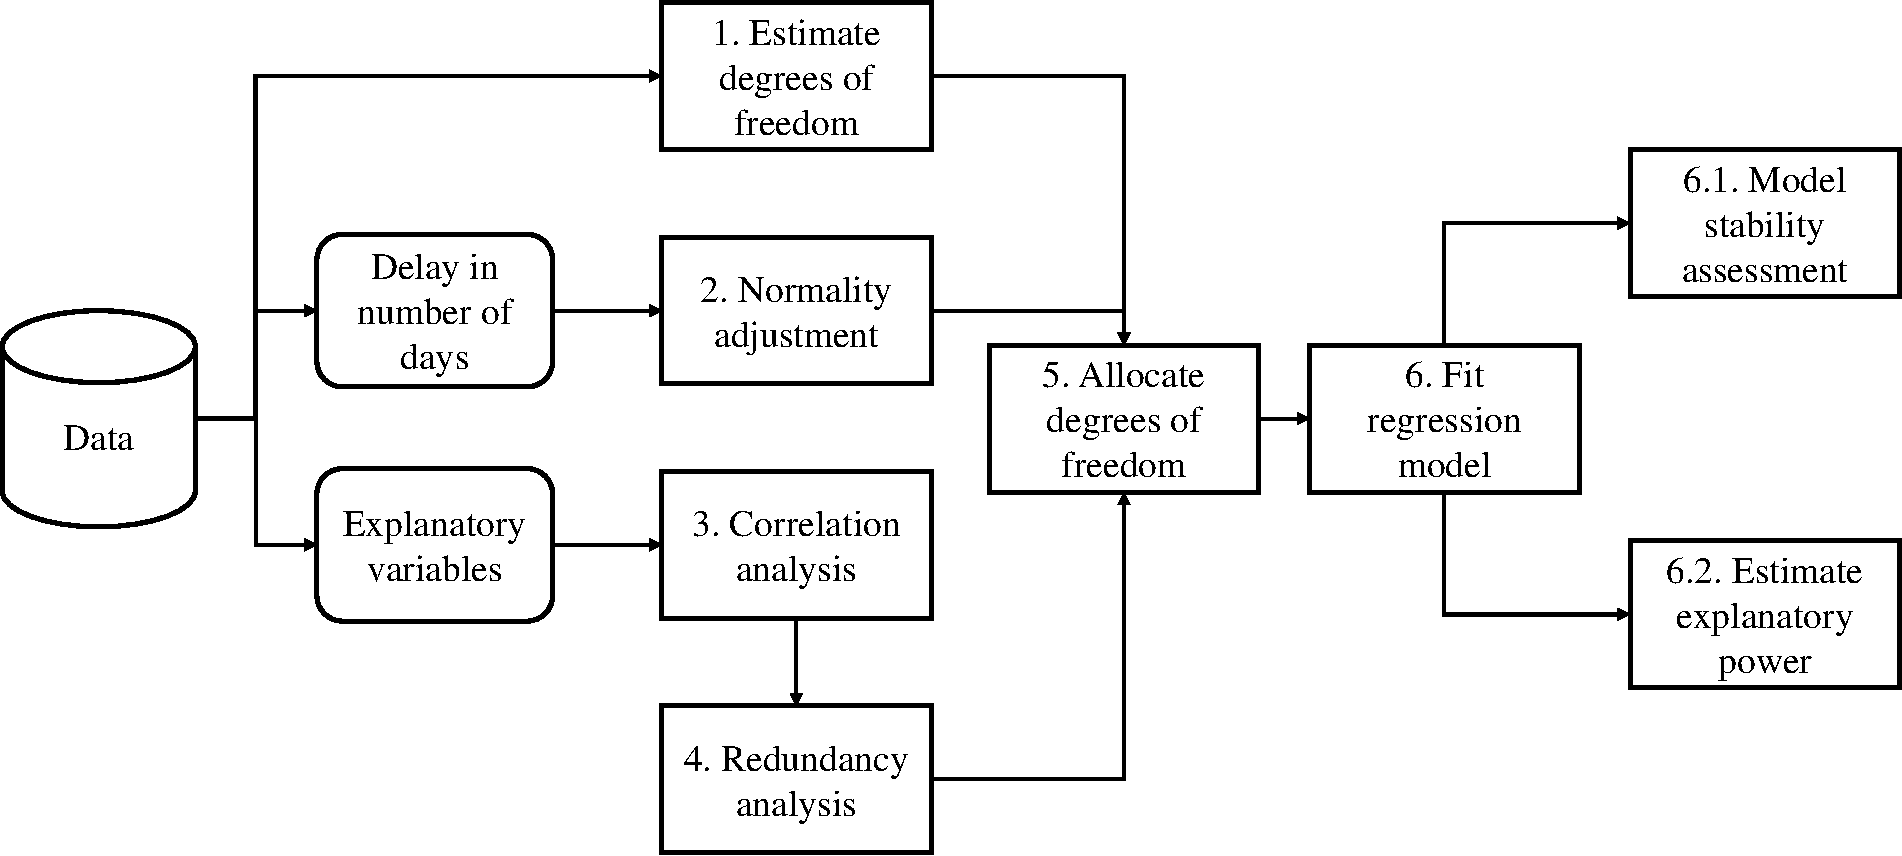
\includegraphics[width=\textwidth,keepaspectratio]
	{chapters/chapter4/figures/linear_model_building_overview}
	\caption{\textbf{Training regression models.} We follow the guidelines
		that are
		provided by Harrell~Jr.~\cite{harrell2001regression} to train regression models, which
	involves nine activities, from data collection to model validation. The
results of Steps 6.2 and is presented in \hyperref[ch4:rq4]{RQ4}.}
	\label{ch4:fig:regression_process}
\end{figure}

We use the guidelines that are provided by
Harrell~Jr.~\cite{harrell2001regression} to fit our regression models.
\hyperref[ch4:fig:regression_process]{Figure}~\ref{ch4:fig:regression_process} provides
an overview of our model fitting approach. In Step~1, we compute the budget of
degrees of freedom that our data can accommodate while keeping the risk of
overfitting low. We compute this budget by using the formula $\frac{n}{15}$
(where $n$ is the number of issues in our dataset). In Step~2, we verify the
normality assumption of \textit{ordinary least squares}, \ie it assumes that the
response variable $y$ should follow normal distribution. Through analysis of the
delivery delay values (\ie the $y$ variable), we find that it does not follow
a normal distribution, and hence, we apply a log transformation $[ln(y+1)]$ to
mitigate such skewness.

In Step~3, we use a variable clustering analysis~\cite{sarle1990varclus} to
remove highly correlated variables. For variables within a cluster that have a
correlation of $|\rho|>0.7$, we choose only one of them to include in our
models---we choose the variable with the least skewed distribution and that we
suspect that shares a stronger relationship with delivery delay. In Step~4, we
check the redundancy of the surviving explanatory variables. Redundant variables
do not add explanatory power to the models and can distort the relationship
between explanatory and response variables. To remove redundant variables we use
the \code{redun} function from the \code{rms} R package, which fits models to
explain each explanatory variable using the other explanatory variables. We then
discard those explanatory variables that could be estimated with an $R^2 \geq
0.9$ (the default threshold of the \code{redun} function).

In the following step (Step~5), we identify which explanatory variables may
benefit from a relaxation of the linear relationship with the response variable.
To identify such variables, we calculate the Spearman multiple $\rho^2$ between
the response and explanatory variables. We spend more of our budgeted degrees of
freedom on the explanatory variables that obtain the higher $\rho^2$ values.

In Step~6, we fit our regression models. In order to assess the fit of our
models (Step~6.1) we use the $R^2$ metric. The $R^2$ measures the {\em
``variability explained''} of the dependent variable that is
analyzed~\cite{steel1960principles}. For instance, a $R^2$ of 0.4 indicates that
40\% of the variability of the dependent variable is being modeled ({\em
``explained''}) by the explanatory variables---the remaining 60\% of the
variability may be due to external factors that are not being modeled or cannot
be controlled. 
%The interpretation of $R^2$ values depends on the analysis that is being
%performed. For example, when prediction is the main goal, the $R^2$ values
%should be very high (\eg around 0.7 to 0.9)~\cite{choi2012predicting}. On the
%other hand, low $R^2$ values (\eg around 0.20) may also generate important
%insights in fields such as psychology or social
%sciences~\cite{bersani2016association}. 

We also use the \textit{Mean Absolute Error} (MAE) to verify how close are the
estimates of our models ($\hat{y}$) to the actual observations ($y$). Then, we
assess the stability of our models by using the \textit{bootstrap-calculated
optimism} of the $R^2$. The \textit{bootstrap-calculated optimism} is computed
by fitting models using bootstrap samples of the original data. For each model
fit to a bootstrap sample, we subtract the $R^2$ of such a model from the model
fit to the original data. This difference is a measure of the \textit{optimism}
in the original model. In this work, we obtain the \textit{bootstrap-calculated
optimism} by computing the average \textit{optimism} obtained using 1,000
bootstrap samples. The smaller the \textit{bootstrap-calculated optimism} the
more stable are our models~\cite{efron1986biased}.

\subsubsection*{\textit{\textbf{RQ3: Results for delivery delay in terms of
releases}}}

\noindent\DIFdelbegin \textit{\textbf{\DIFdel{Our explanatory models obtain a median precision of 0.81 to
0.88 and a median recall of 0.29 to 0.92.}}%DIFAUXCMD
}
%DIFAUXCMD
\DIFdelend \DIFaddbegin \finding{Our explanatory models obtain a median precision of 0.81 to
0.88 and a median recall of 0.29 to 0.92.}{find6}
\DIFaddend \hyperref[ch4:fig:RFclassificationResult]{Figure}~\ref{ch4:fig:RFclassificationResult}
shows the precision, recall, F-measure, and AUC of our explanatory models.  The
bar charts show the values that we observe for each bucket. The values of
precision, recall, F-measure, and AUC are also shown in
\hyperref[ch4:tbl:evaluation_metrics]{Table}~\ref{ch4:tbl:evaluation_metrics}. 

\begin{figure}
	\centering
	%\captionsetup{justification=centering}
	\subfloat[Eclipse]{
		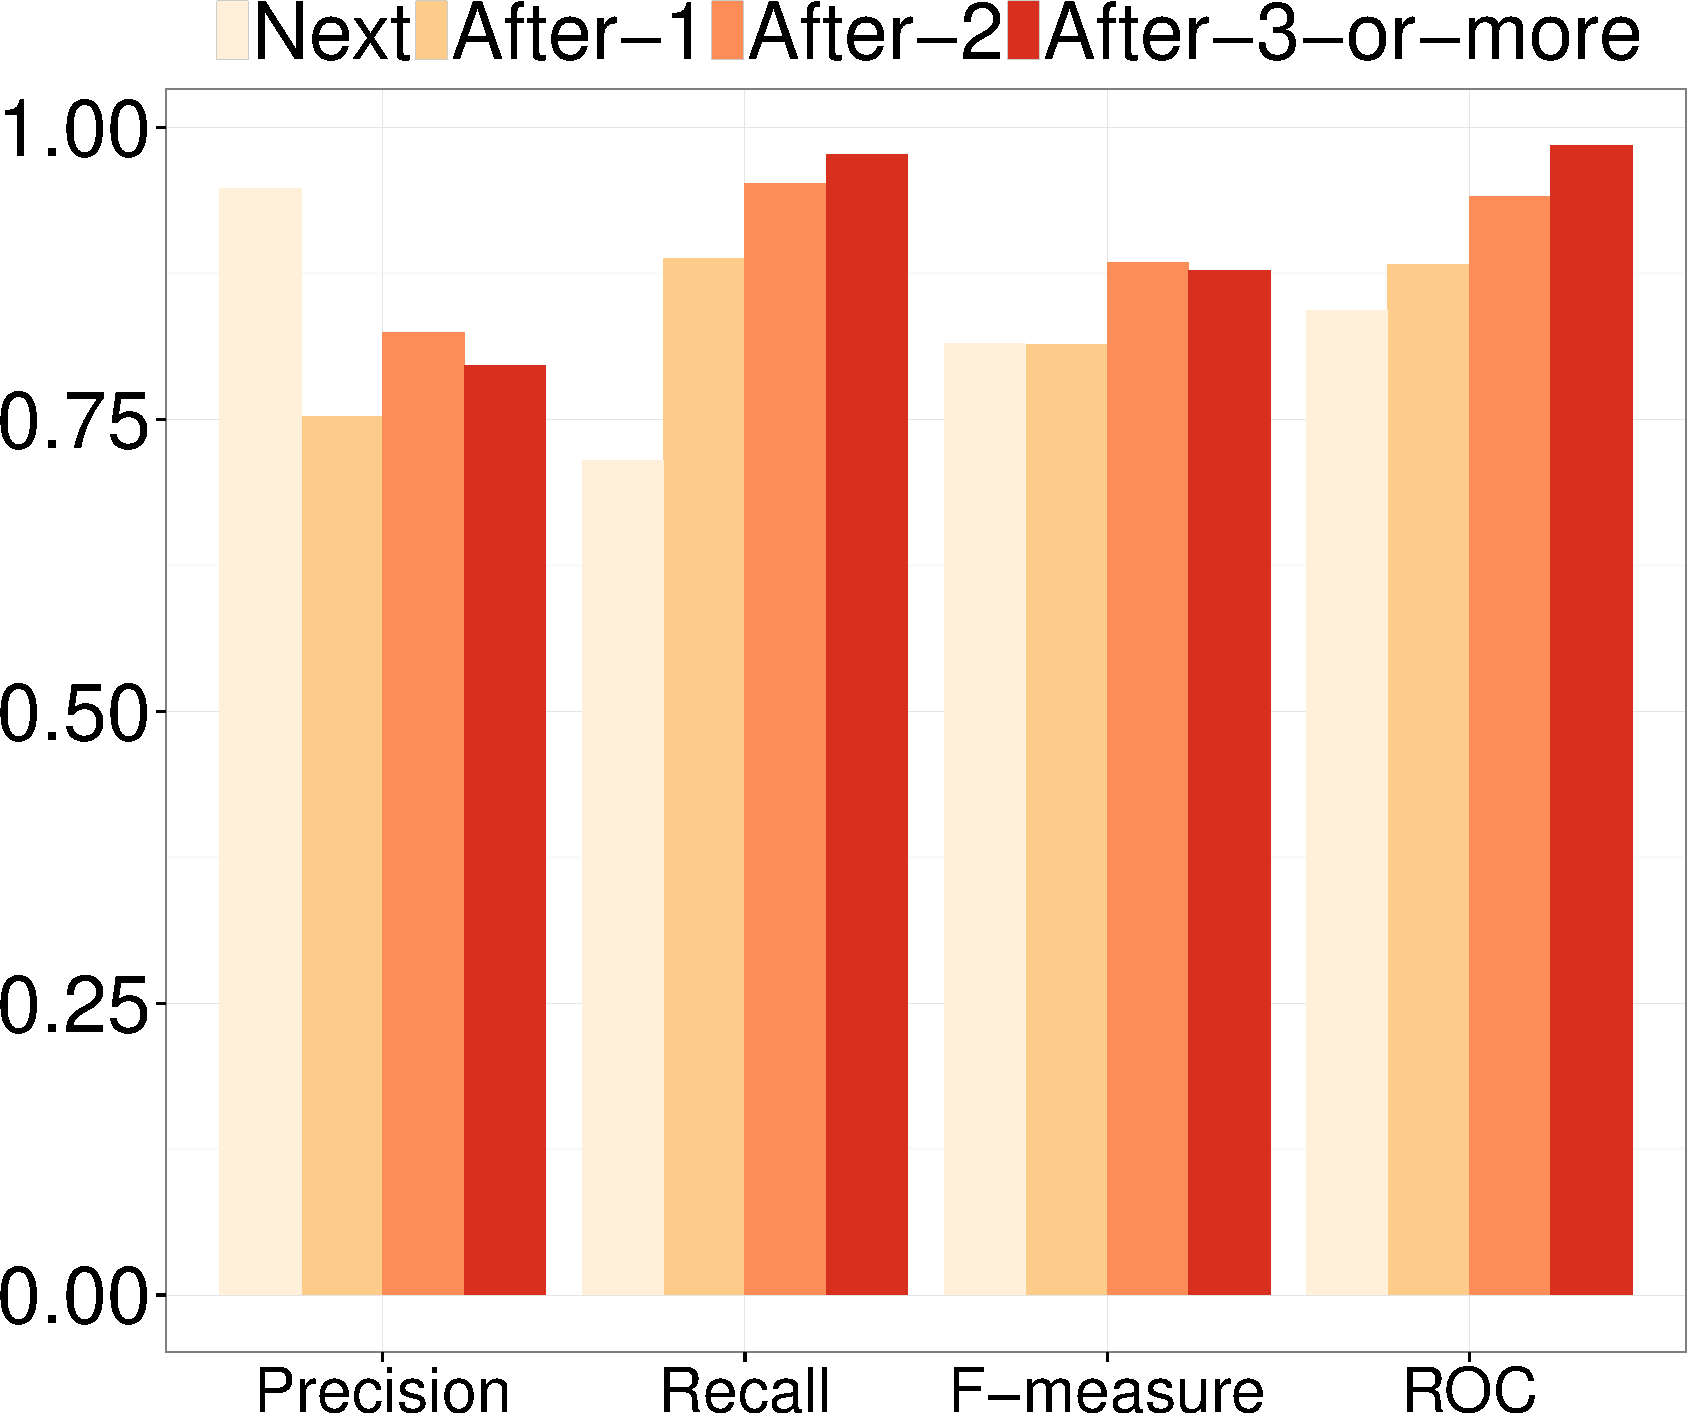
\includegraphics[width=0.50\textwidth,keepaspectratio] 
		{chapters/chapter4/figures/eclipse_loocv_evaluation.pdf}
		\label{ch4:fig:RFeclipse}
	}

	\subfloat[Firefox]{
		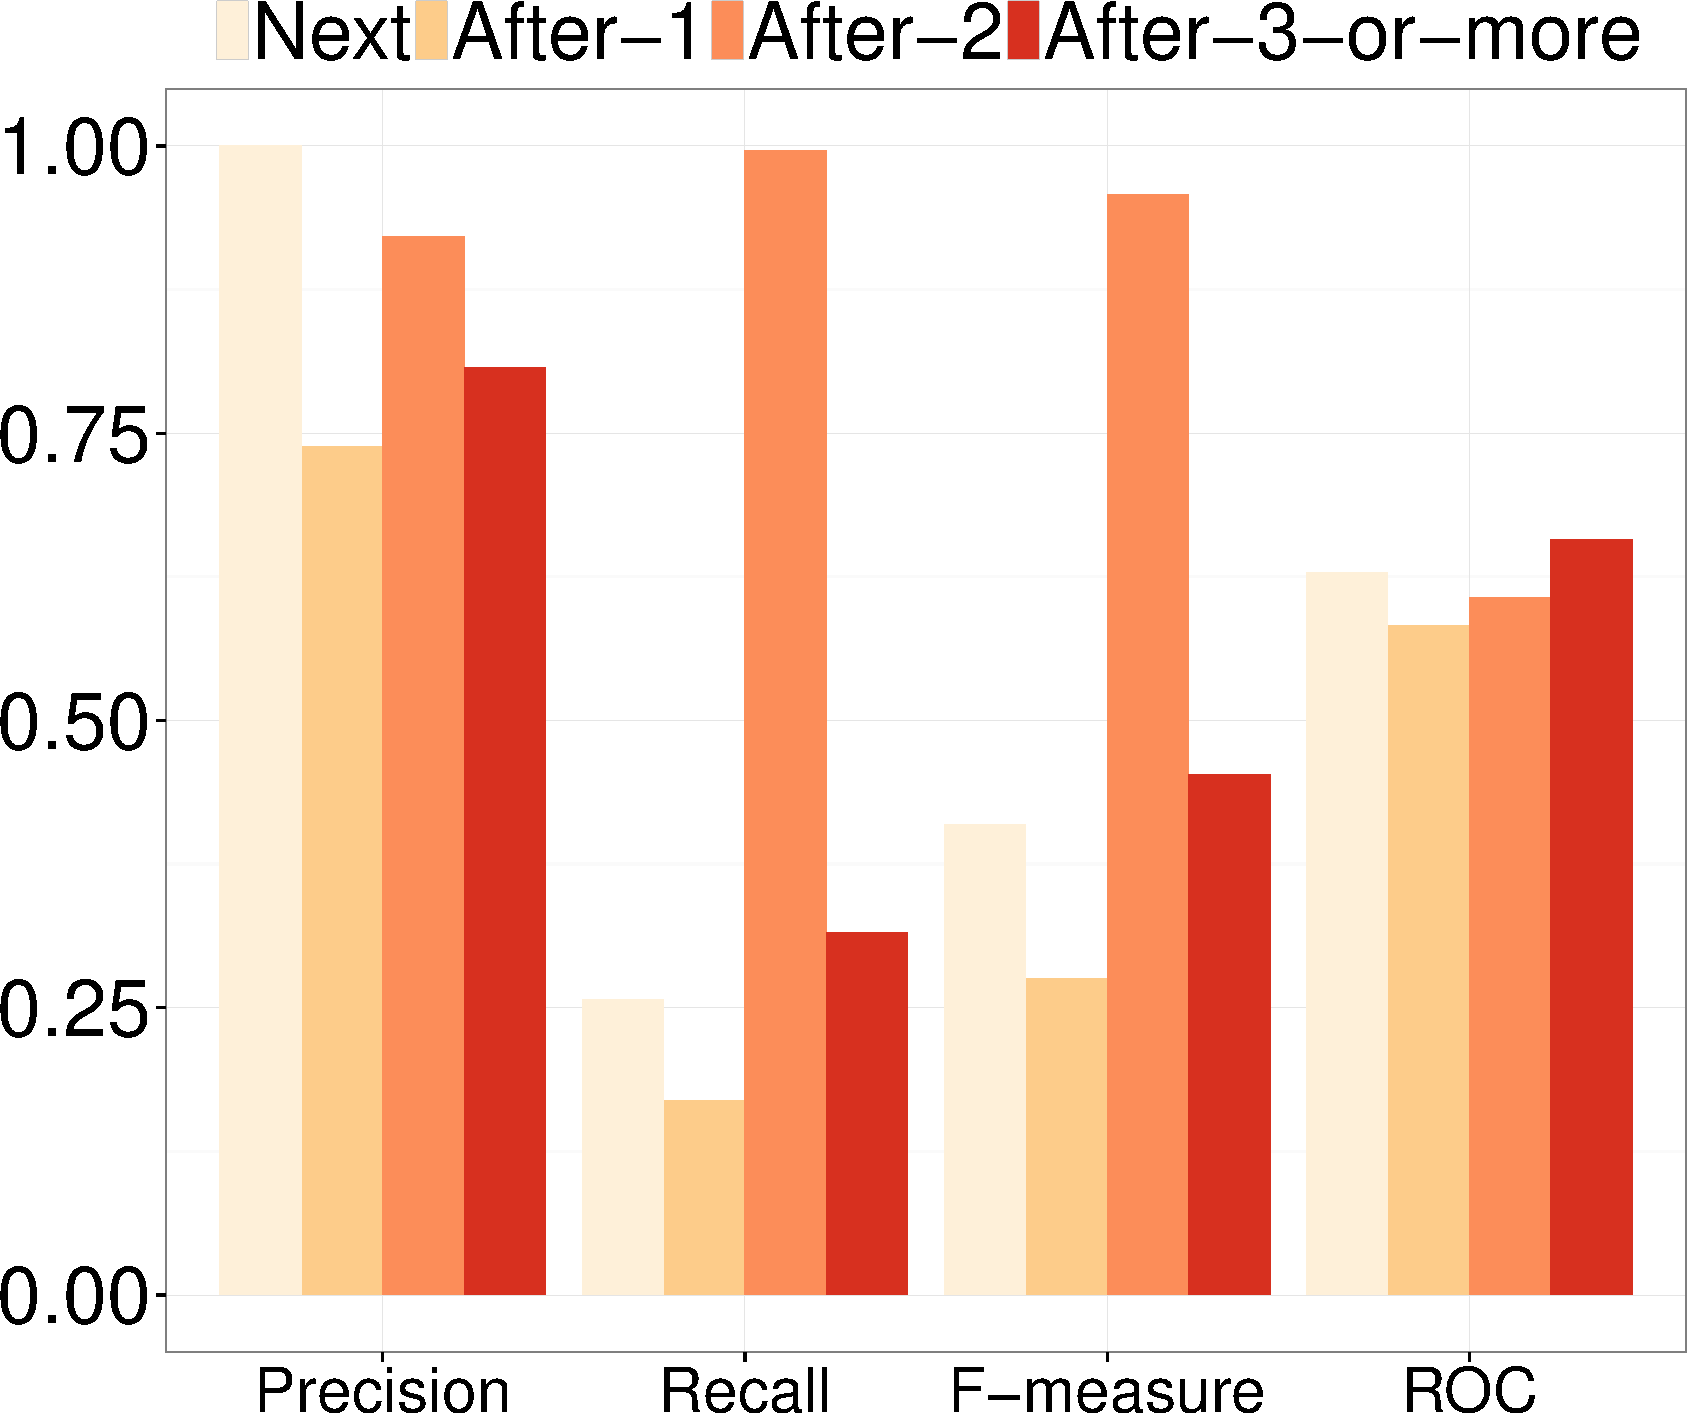
\includegraphics[width=0.50\textwidth,keepaspectratio]  
		{chapters/chapter4/figures/firefox_loocv_evaluation.pdf}
		\label{ch4:fig:RFfirefox}
	}

	\subfloat[ArgoUML]{
		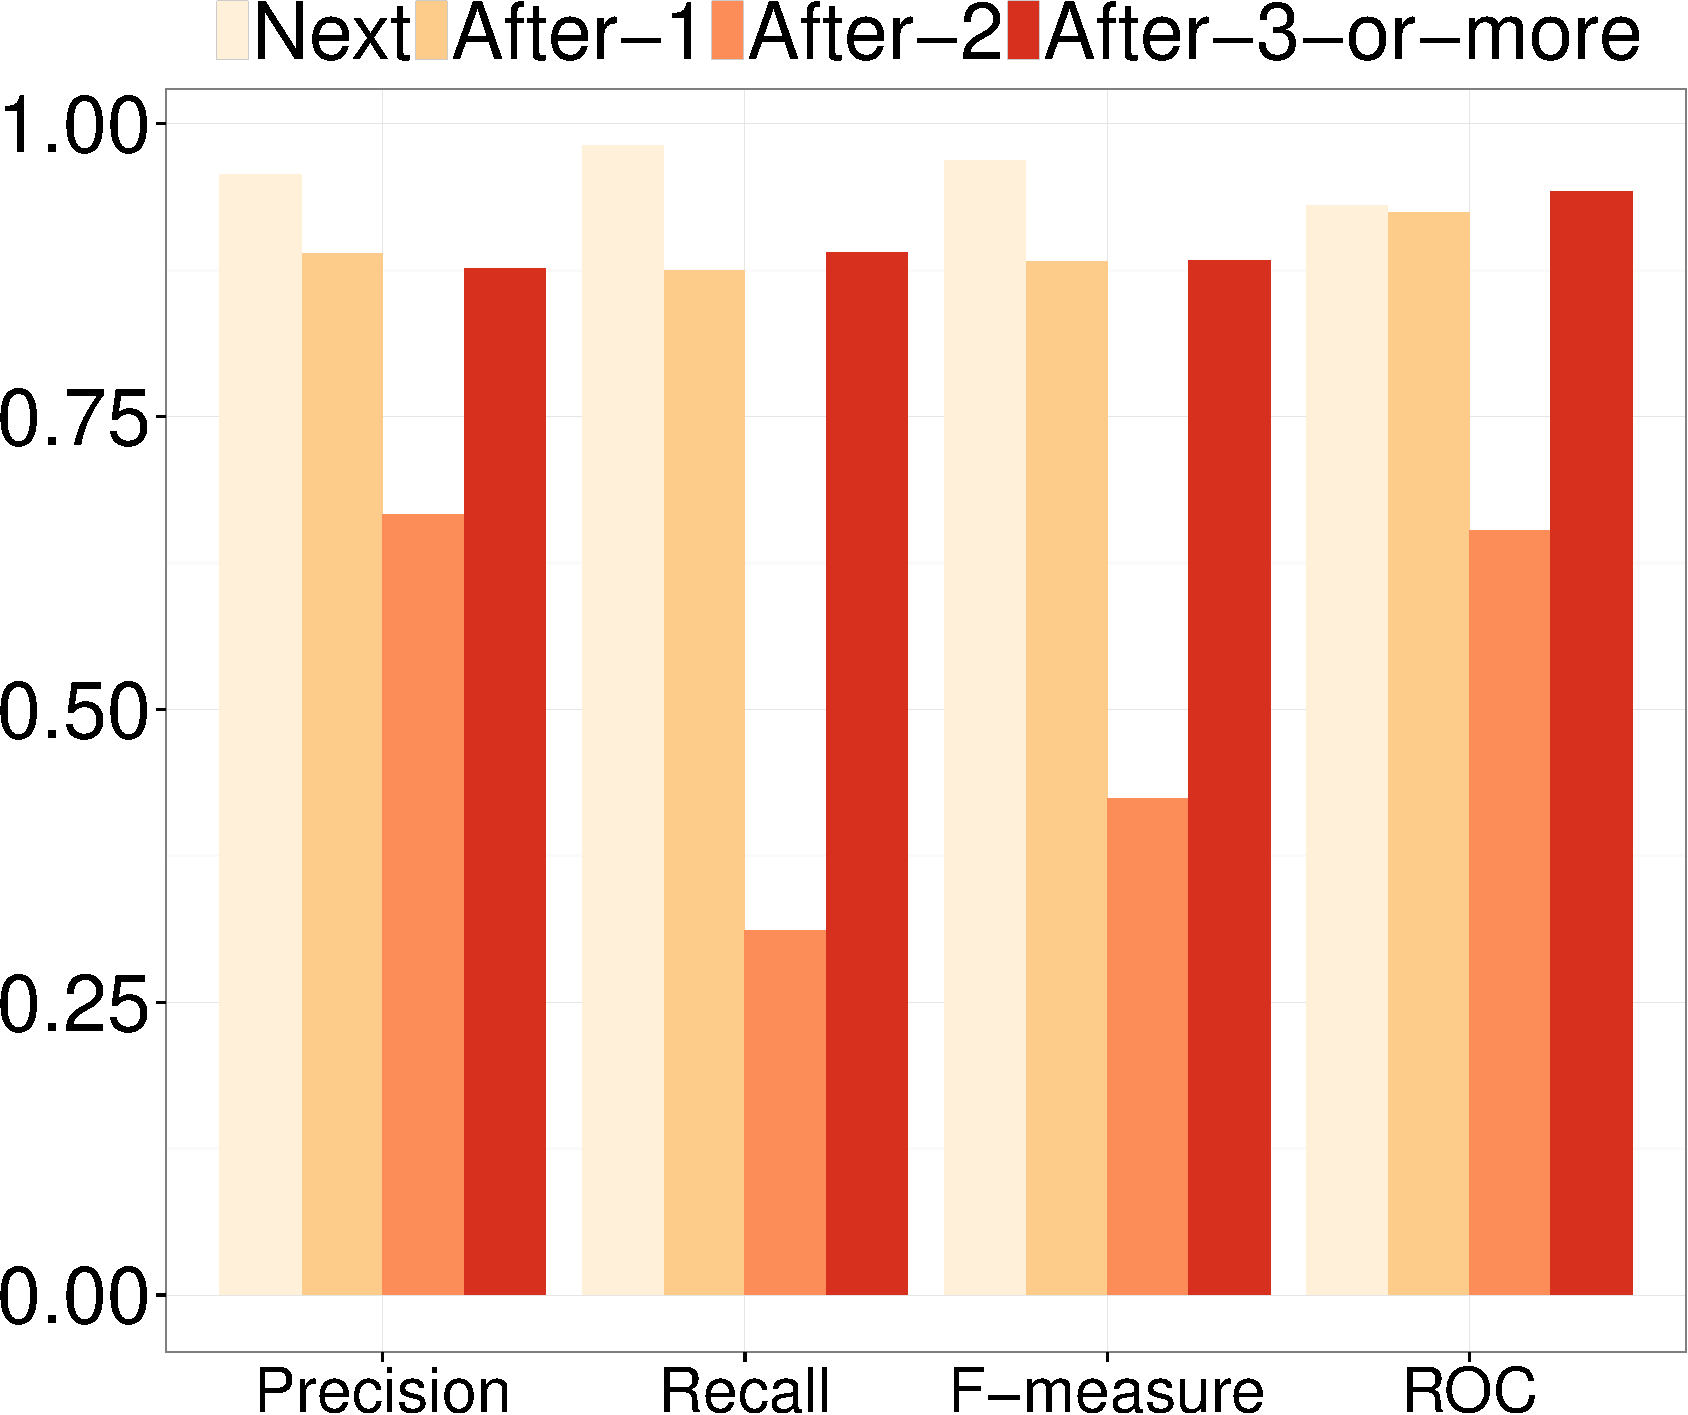
\includegraphics[width=0.50\textwidth,keepaspectratio] 
		{chapters/chapter4/figures/argouml_loocv_evaluation.pdf}
		\label{ch4:fig:RFargo}
	}
	\caption{\textbf{Performance of random forest models.} We show the
	values of Precision, Recall, F-measure, and AUC that are
computed using the LOOCV technique.}
	\label{ch4:fig:RFclassificationResult}
\end{figure}

\begin{table}
	\footnotesize
	\centering
	\caption{The precision, recall, F-measure, and AUC values that are
	obtained for the Eclipse, Firefox, and ArgoUML projects. 
	\label{ch4:tbl:evaluation_metrics}
	}
	\begin{tabular}{lcccc}
		\hline
		\multicolumn{5}{c}{\textbf{Eclipse}}\tabularnewline
		\hline 
		\textbf{Bucket} & \textbf{Precision} & \textbf{Recall} &
		\textbf{F-measure} & \textbf{AUC}\tabularnewline
		\hline 
		Next & 0.95  & 0.71  & 0.81 & 0.84 \tabularnewline
		\hline 
		After-1 & 0.75 & 0.89 & 0.81 & 0.88\tabularnewline
		\hline 
		After-2 & 0.82 & 0.95 & 0.88 & 0.94\tabularnewline
		\hline 
		After-3-or-more & 0.80 & 0.98 & 0.88 & 0.98\tabularnewline
		\hline 
		\hline
		\multicolumn{5}{c}{\textbf{Firefox}}\tabularnewline
		\hline 
		\textbf{Bucket} & \textbf{Precision} & \textbf{Recall} &
		\textbf{F-measure} & \textbf{AUC}\tabularnewline
		\hline 
		Next & 0.99  & 0.26  & 0.41 & 0.63 \tabularnewline
		\hline 
		After-1 & 0.74 & 0.17 & 0.28 & 0.58\tabularnewline
		\hline 
		After-2 & 0.92 & 0.99 & 0.96 & 0.61\tabularnewline
		\hline 
		After-3-or-more & 0.81 & 0.32 & 0.45 & 0.66\tabularnewline
		\hline 
		\hline
		\multicolumn{5}{c}{\textbf{ArgoUML}}\tabularnewline
		\hline 
		\textbf{Bucket} & \textbf{Precision} & \textbf{Recall} &
		\textbf{F-measure} & \textbf{AUC}\tabularnewline
		\hline 
		Next & 0.96  & 0.98  & 0.97 & 0.93 \tabularnewline
		\hline 
		After-1 & 0.89 & 0.87 & 0.88 & 0.92\tabularnewline
		\hline 
		After-2 & 0.67 & 0.31 & 0.42 & 0.65\tabularnewline
		\hline 
		After-3-or-more & 0.88 & 0.89 & 0.88 & 0.94\tabularnewline
		\hline 
	\end{tabular}
\end{table}

The best precision/recall values that we obtain for the Eclipse, Firefox, and
ArgoUML projects are related to the \textit{after-2} (F-measure of 0.88),
\textit{after-2} (F-measure of 0.96), and \textit{next} (F-measure of 0.97),
respectively. However, for buckets with low number of instances,
precision/recall values decrease considerably. For instance, the F-measures that
are obtained by our models for the Firefox project are considerably low for the
\textit{next}, \textit{after-1}, and \textit{after-3-or-more} buckets (0.41,
0.28 and 0.45, respectively).

Moreover, our models obtain median AUCs between 0.62 to 0.96, which indicate
that our model estimations are better than random guessing (AUC of 0.5).
Summarizing the results, our models obtain a median precision of 0.81-0.88
(median) and a median recall of 0.29-0.92. Our models provide a sound starting
point for studying the release into which an addressed issue will be \DIFdelbegin \DIFdel{integrated}\DIFdelend \DIFaddbegin \DIFadd{delivered}\DIFaddend .\\

\noindent\DIFdelbegin \textit{\textbf{\DIFdel{Our models obtain better F-measure values than
Zero-R.}}%DIFAUXCMD
} %DIFAUXCMD
\DIFdelend \DIFaddbegin \finding{Our models obtain better F-measure values than
Zero-R.}{find7} \DIFaddend We compared our models to Zero-R models as a baseline. For all test
instances, Zero-R selects the bucket that contains the majority of the instances.
Hence, the recall for the bucket containing the majority of instances is 1.0. We
compared the F-measure of our models to the F-measure of Zero-R models. We
choose to compare to the F-measure values because precision and recall are very
skewed for Zero-R. 

For the Firefox project, Zero-R obtains an F-measure of 0.95 for the
\textit{after-2} bucket, whereas our model obtains an F-measure of 0.96 for the
same bucket. For the Eclipse project, Zero-R always selects \textit{next} and
obtains a F-measure of 0.58, while our model obtains an F-measure of 0.81.
Finally, for the ArgoUML project, Zero-R always selects \textit{next} with an
F-measure of 0.84, whereas our model obtains an F-measure of 0.97. These results
show that our models yield better F-measure values than na\"{i}ve techniques
like Zero-R or random guessing (AUC = 0.5) in the majority of cases.  

\DIFdelbegin %DIFDELCMD < \conclusionbox{We are able to accurately model how many releases an addressed issue
%DIFDELCMD < is likely to be prevented from integration. Our models outperform na\"{i}ve
%DIFDELCMD < techniques, such as Zero-R and random guessing, obtaining AUC values of 0.62 to
%DIFDELCMD < 0.96.}
%DIFDELCMD < %%%
\DIFdelend \DIFaddbegin \conclusionbox{We are able to accurately model how many releases an addressed issue
is likely to be prevented from delivery. Our models outperform na\"{i}ve
techniques, such as Zero-R and random guessing, obtaining AUC values of 0.62 to
0.96.}
\DIFaddend 

\begin{table}
	\centering
	\footnotesize
	\caption{\textbf{Regression results of model fit.} Our explanatory
		models obtain $R^2$ values between 0.39 to 0.65 and MAE values between
	7.8 to 66 days.}
	\label{ch4:tbl:regression_results}
	\def\arraystretch{1.5}
	\begin{tabular}{lrrr}
		\hline 
		\centering{\textbf{Metric/Project}} &
		\centering{\textbf{Eclipse}} & \centering{\textbf{Firefox}} &
		\centering{\textbf{ArgoUML}} \tabularnewline
		\hline 
		$R^2$ & 0.48  & 0.39 & 0.65 \tabularnewline
		\hline 
		MAE (days) & 61 & 7.8  & 66 \tabularnewline
		\hline 
		Release cycle duration (median in days) & 112 & 42 & 180 \tabularnewline
		\hline
		Error ratio $(\frac{MAE}{cycle})$ & 0.54  & 0.18  & 0.37 \tabularnewline
		\hline 
		Optimism & 0.0267 & 0.0162 & 0.0035 \tabularnewline
		\hline 
	\end{tabular}
\end{table}

\subsubsection*{\textit{\textbf{RQ3: Results for delivery delay in terms of days}}}

\noindent\DIFdelbegin \textbf{\textit{\DIFdel{Our explanatory models obtain $R^2$ values of 0.39-0.65
and MAE values between 7.8 to 67 days.}}%DIFAUXCMD
} %DIFAUXCMD
\DIFdelend \DIFaddbegin \finding{Our explanatory models obtain $R^2$ values of 0.39-0.65
and MAE values between 7.8 to 67 days.}{find8} \DIFaddend Our models obtain fair $R^2$ values to
model the variability of delivery delay in days in the studied projects.
\hyperref[ch4:tbl:regression_results]{Table}~\ref{ch4:tbl:regression_results} shows the
$R^2$ and MAE values that are obtained by each of our regression models. The
$R^2$ values for the Eclipse, Firefox, and ArgoUML projects are of 0.39, 0.48,
and 0.65, respectively. 
Additionally, our regression models can provide fair
estimations of delivery delay in days, specially for the Firefox project. For
instance, the median interval in days between releases of the Firefox project is
42 days
(see~\hyperref[ch4:fig:releaseIntervals]{Figure}~\ref{ch4:fig:releaseIntervals}), while
the MAE value for the Firefox project is 7.8 days, which equates to an error
ratio of 18\% (see
\hyperref[ch4:tbl:regression_results]{Table}~\ref{ch4:tbl:regression_results}).\\

\noindent\DIFdelbegin \textbf{\textit{\DIFdel{Our explanatory models obtain a good stability with bootstrap
calculated optimism between 0.0035 to 0.0267 of the $R^2$ values.}}%DIFAUXCMD
} %DIFAUXCMD
\DIFdelend \DIFaddbegin \finding{Our explanatory models obtain a good stability with bootstrap
calculated optimism between 0.0035 to 0.0267 of the $R^2$ values.}{find9} \DIFaddend We also
observe that our regression models are stable.
\hyperref[ch4:tbl:regression_results]{Table}~\ref{ch4:tbl:regression_results} shows the
\textit{bootstrap-calculated} optimism of the $R^2$ values of our models. The
optimism for the Eclipse, Firefox and ArgoUML projects are 0.0267, 0.0162, and 0.0035,
respectively. Such results indicate that our explanatory models are unlikely to
be overfitted to our data and that our models are stable enough for us to perform the
statistical inferences that follow. 

\conclusionbox{We are able to accurately estimate the delivery delay in terms
of number of days. Our models obtain fair $R^2$ values of 0.39 to 0.65. Our
exploratory models are quite stable with a maximum optimism of 0.0267.}

\subsection{RQ4: What are the most influential attributes for
modeling delivery delay?}\label{ch4:rq4}

\subsubsection*{RQ4: Motivation} In \hyperref[ch4:rq3]{RQ3}, we found that our
models can accurately model the delivery delay of addressed issues. To fit our
models, we use attributes that we collect from ITSs and VCSs. As described in
\hyperref[ch4:tbl:dimensions]{Tables}~\ref{ch4:tbl:dimensions},~\ref{ch4:tbl:dimensions2}
and~\ref{ch4:tbl:dimensions3}, the attributes belong to different families that
are related to addressed issues. In \hyperref[ch4:rq4]{RQ4}, we investigate
which attributes are influential to estimate the delivery delay of addressed
issues. We present the approaches and results of \hyperref[ch4:rq4]{RQ4} for
each studied type of delivery delay (\hyperref[def:1]{Definitions}~\ref{def:1}
and~\ref{def:2}). 

\subsubsection*{RQ4: Approach}

To identify the most influential attributes for estimating the delivery delay
in terms of releases (\hyperref[def:1]{Definition}~\ref{def:1}), we compute the
\textit{variable importance} score for each attribute of our models. The
\textit{variable importance} implementation that we use in our study is
available within the \textit{bigrf} R package. This implementation computes the
importance score based on {\em Out Of the Bag} (OOB) estimates. Each attribute
of the dataset is randomly permuted in the OOB data.  Then, the average \(a\) of
the differences between the votes for the correct bucket in the permuted OOB and
the original OOB is computed. The result of \(a\) is the importance of an
attribute. 

The final output of the variable importance is a rank of the attributes
indicating their importance for the model. Hence, if a specific attribute has
the highest rank, then it is the most influential attribute that our explanatory
model is using to estimate delivery delay. Finally, we use the models with the
largest training corpus when performing the LOOCV to compute the variable
importance scores.

We perform Step~6.2 of
\hyperref[ch4:fig:regression_process]{Figure}~\ref{ch4:fig:regression_process} to
identify the most influential attributes in our models that we fit to study the
delivery delay in terms of number of days
(\hyperref[def:2]{Definition}~\ref{def:2}). We evaluate the explanatory power of
each attribute by using the Wald $\chi^2$ maximum likelihood test (Step~6.2).
The larger the $\chi^2$ value, the greater the power that a particular attribute
has to model the variability of delivery delay in terms of days. To do so, we
use the \code{anova} function of the \code{rms} R package.

\subsubsection*{\textit{\textbf{RQ4: Results for delivery delay in terms of
releases}}}

\noindent\DIFdelbegin \textit{\textbf{\DIFdel{The fixing time per resolver and integration workload
attributes are the most influential attributes in our models.}}%DIFAUXCMD
}
%DIFAUXCMD
\DIFdelend \DIFaddbegin \finding{The fixing time per resolver and integration workload
attributes are the most influential attributes in our models.}{find10}
\DIFaddend \hyperref[ch4:fig:variableImportance]{Figure}~\ref{ch4:fig:variableImportance} shows the
variable importance values of the LOOCV of our models. The most influential
attribute is the \textit{fixing time per resolver}. The \textit{fixing time per
resolver} attribute measures the total time that is spent by each resolver on
fixing issues in a release cycle. The second most influential attributes are
integration workload attributes (\ie backlog of issues and backlog of issues per
resolver). These integration workload attributes measure the competition of
issues that were addressed but not yet \DIFdelbegin \DIFdel{integrated into }\DIFdelend \DIFaddbegin \DIFadd{delivered through }\DIFaddend an official release.

\begin{figure}
	\center
	\subfloat[Eclipse]{
		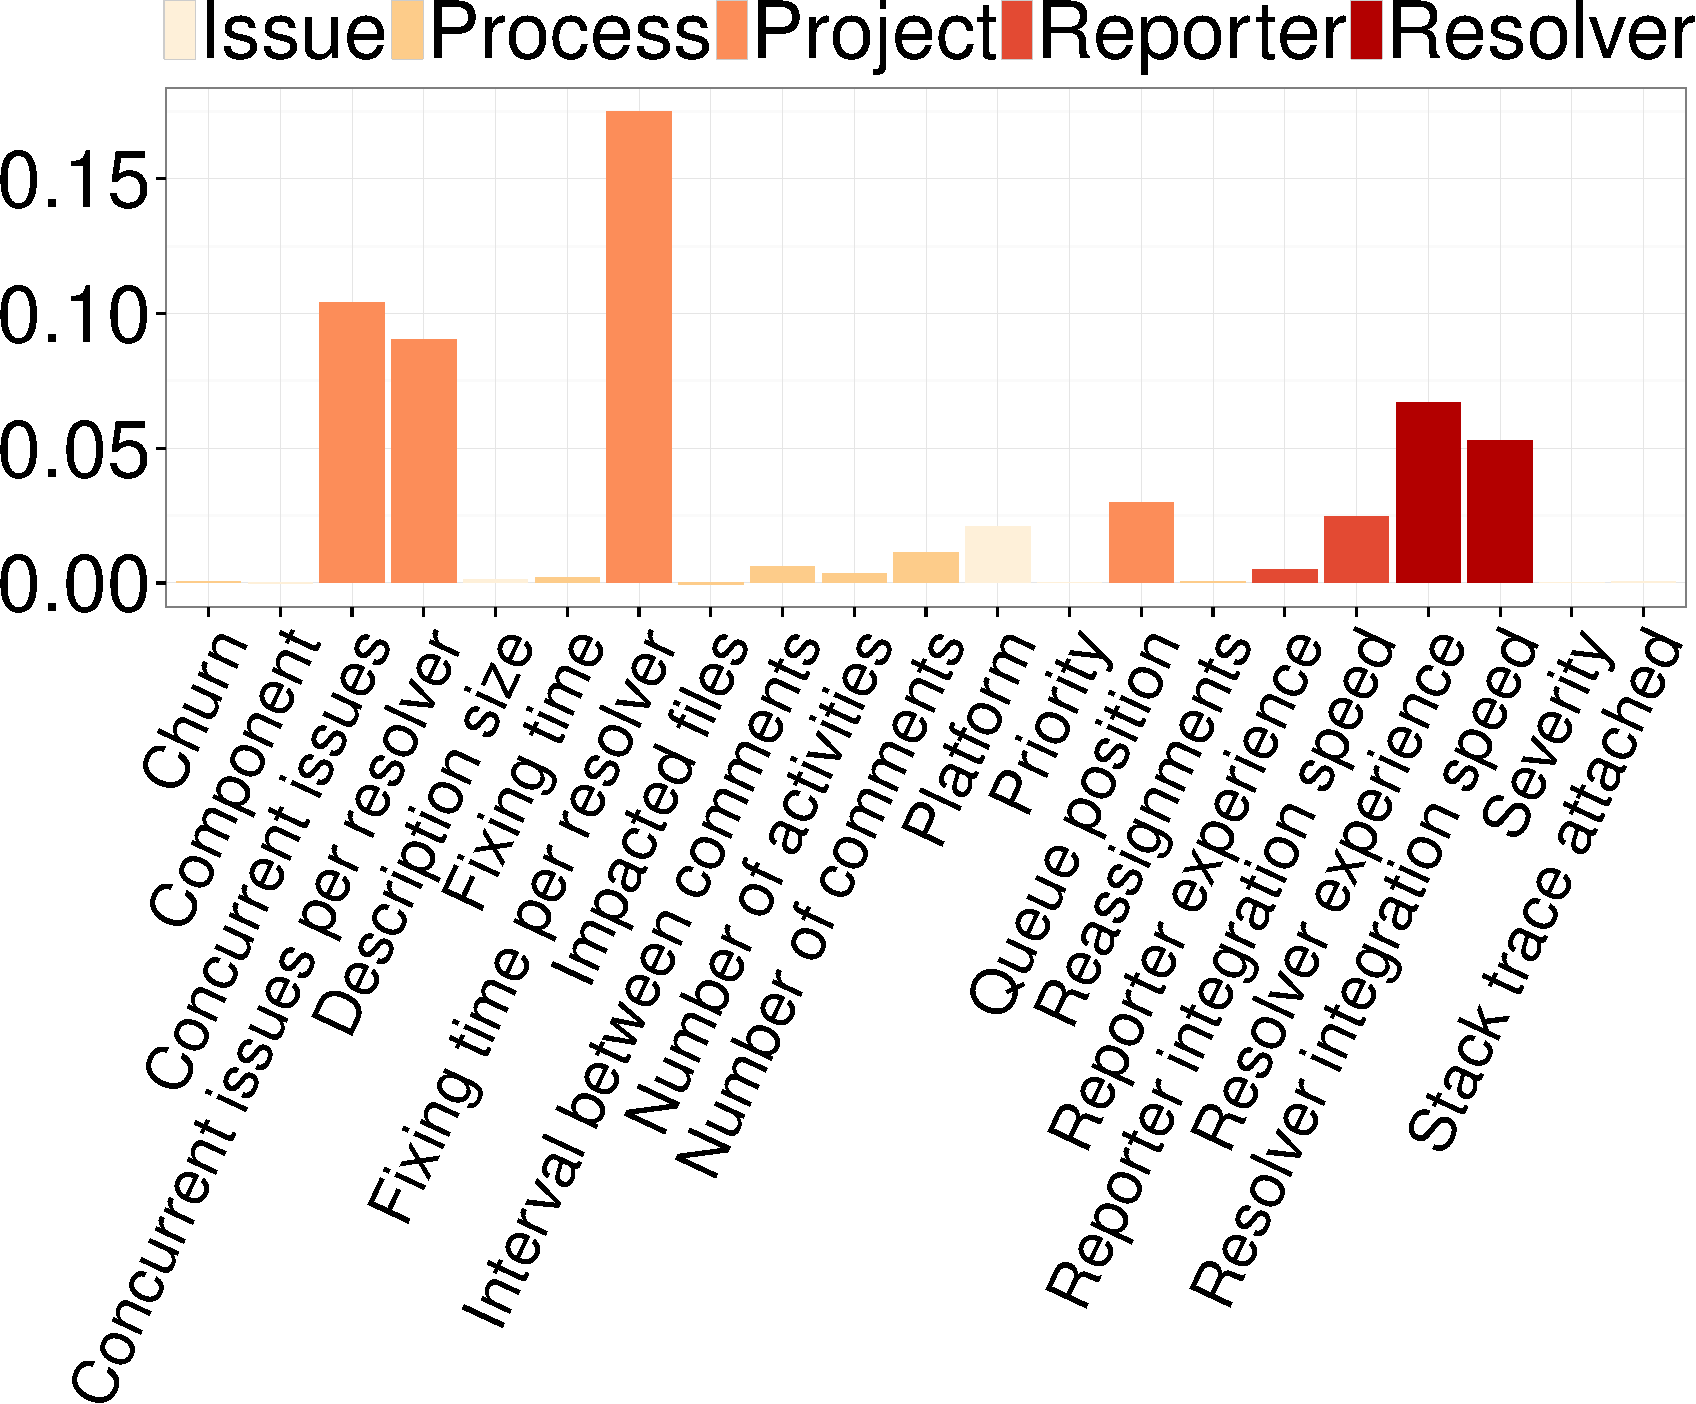
\includegraphics[width=0.55\textwidth,keepaspectratio] 
		{chapters/chapter4/figures/eclipse_loocv_varimp.pdf}
	\label{ch4:fig:impEclipse}
	}

	\subfloat[Firefox]{
		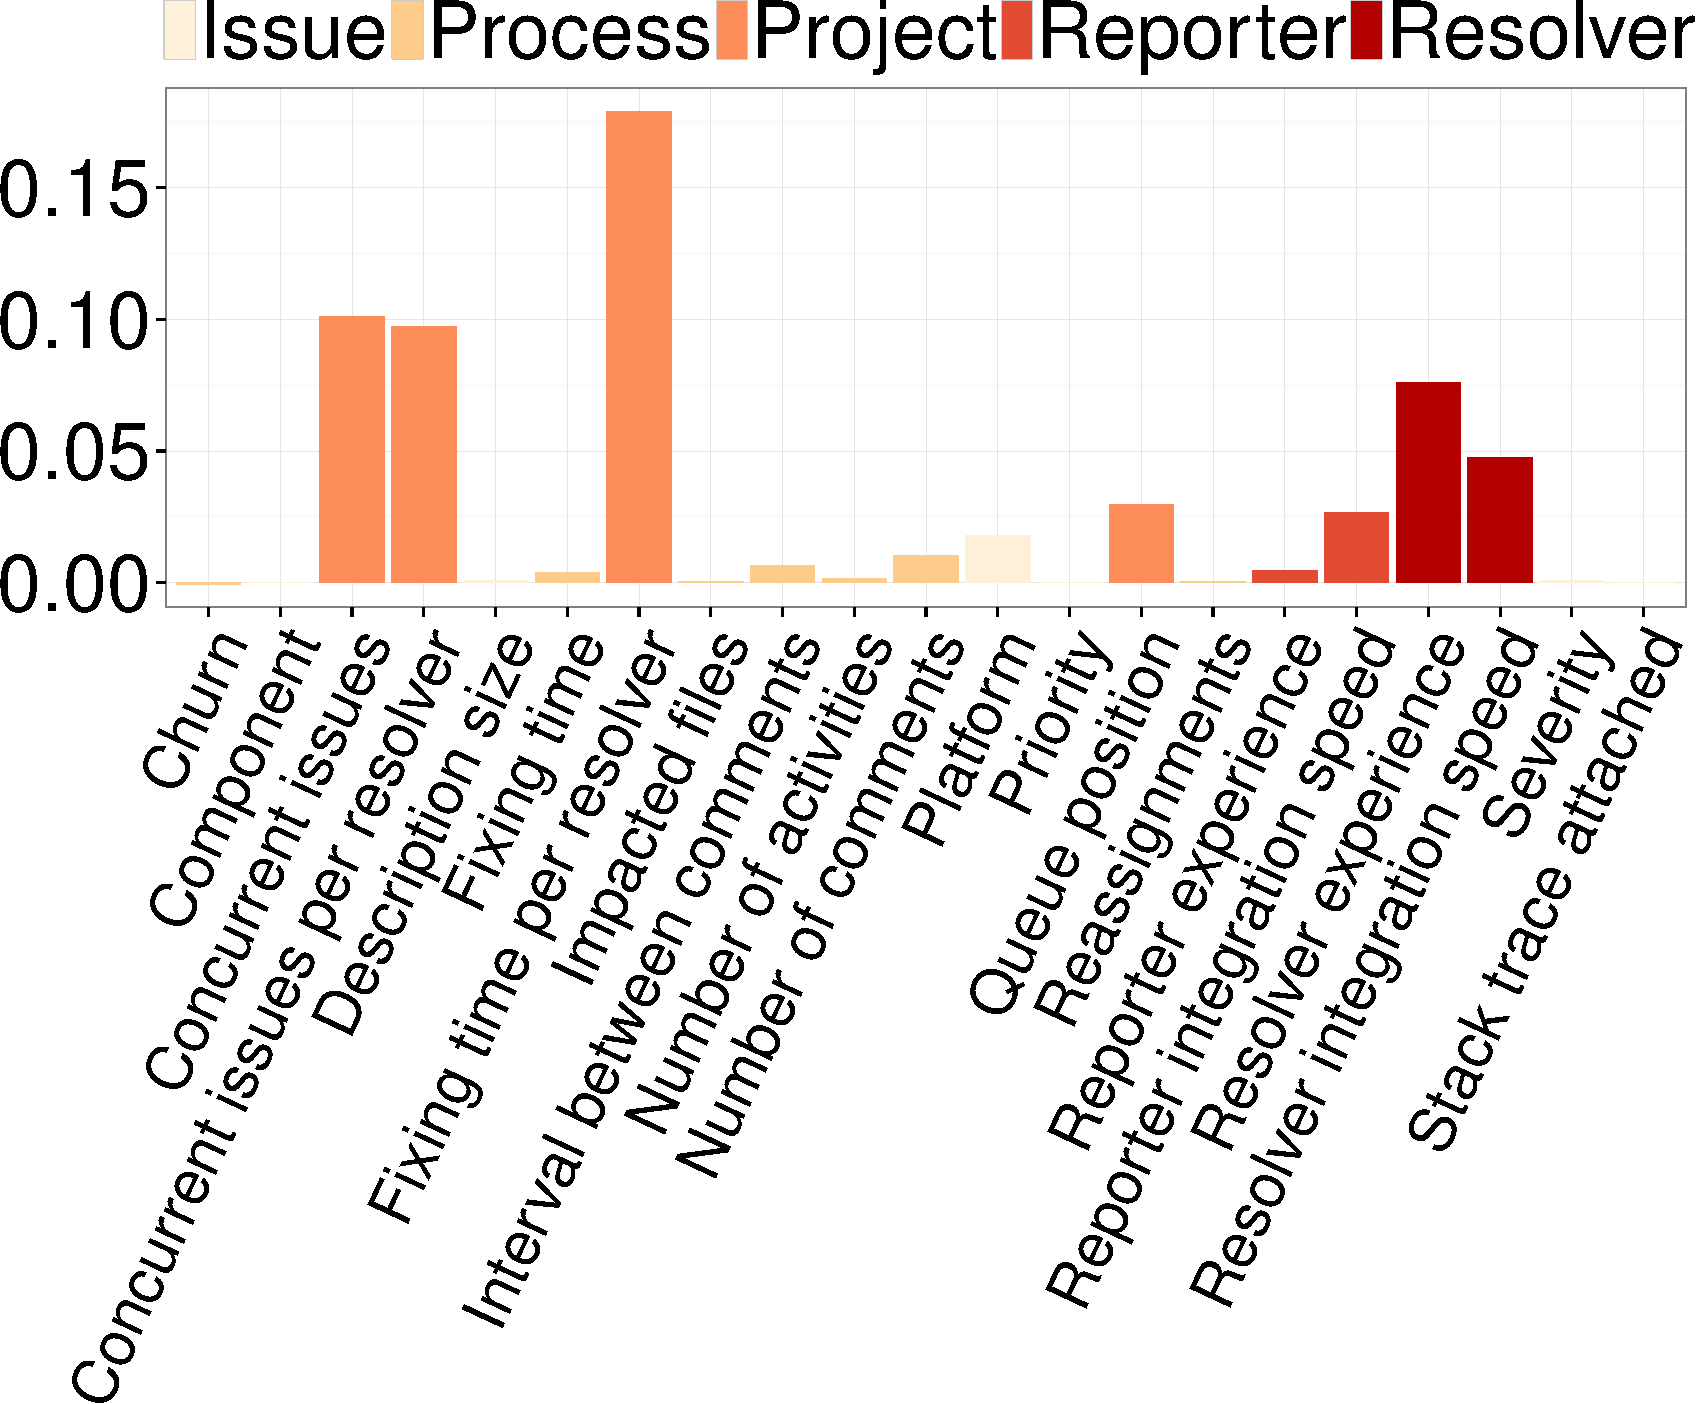
\includegraphics[width=0.55\textwidth,keepaspectratio]  
		{chapters/chapter4/figures/firefox_loocv_varimp.pdf}
		\label{ch4:fig:impFirefox}
	}

	\subfloat[ArgoUML]{
		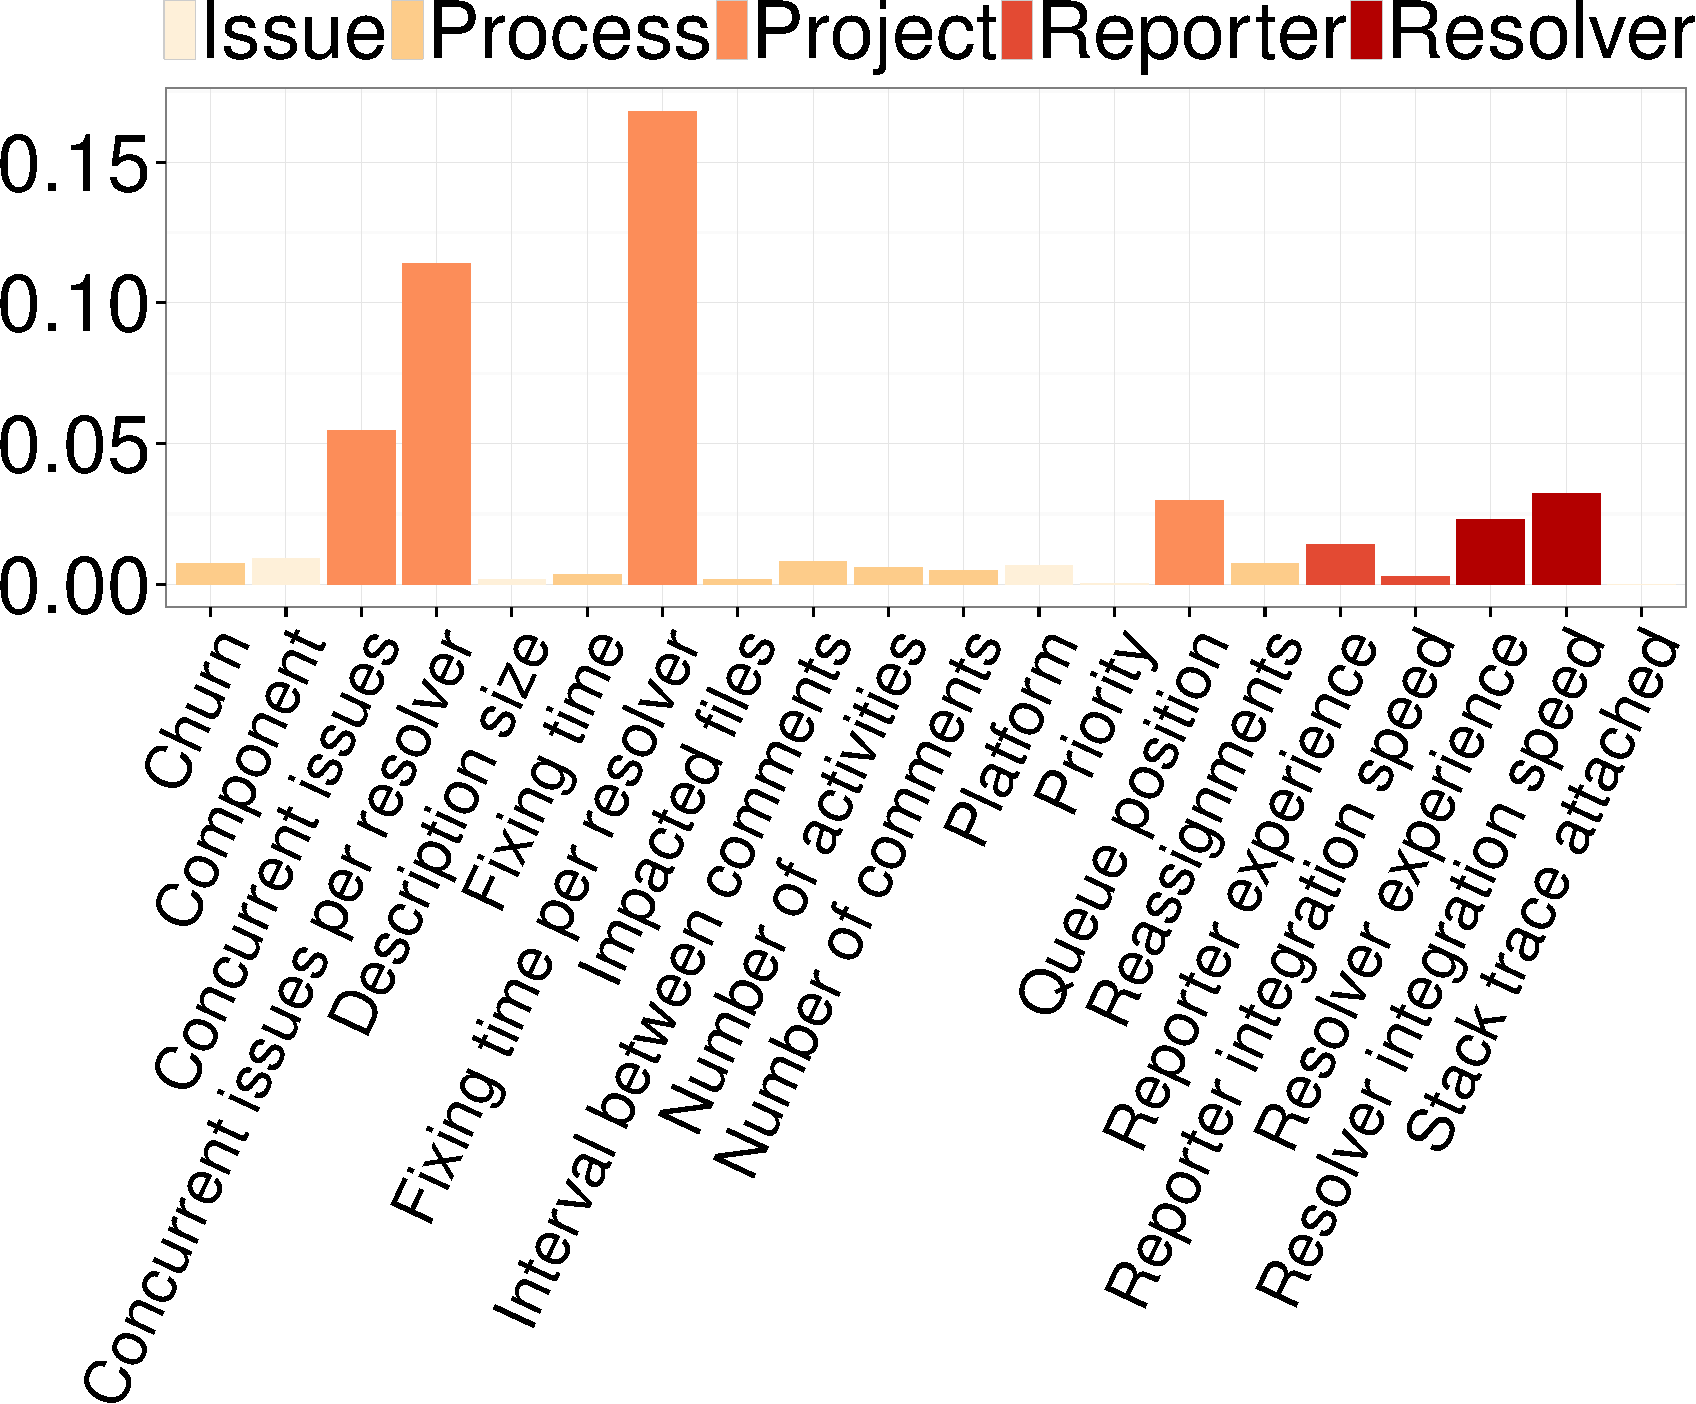
\includegraphics[width=0.55\textwidth,keepaspectratio] 
		{chapters/chapter4/figures/argouml_loocv_varimp.pdf}
	\label{ch4:fig:impArgo}}
	\caption{\textbf{Variable importance scores.} We show the 
		importance scores that are computed for the LOOCV of our models.}
	\label{ch4:fig:variableImportance}
\end{figure}

Our results suggest that the time that is invested by the resolvers on fixing
issues have a strong association with delivery delay. This could be due to
resolvers fixing issues more carefully---which would lead to a smoother
\DIFdelbegin \DIFdel{integration }\DIFdelend \DIFaddbegin \DIFadd{delivery }\DIFaddend of such issues---or issues that were less complex in overall (\eg a
shorter time was invested), which might simplify the \DIFdelbegin \DIFdel{integration }\DIFdelend \DIFaddbegin \DIFadd{delivery }\DIFaddend process. A deeper
analysis of this attribute would be necessary to better understand the exact
reasons behind this relationship (\eg consulting the development team through
surveys and interviews). 

We also observe that integration workload attributes (\ie \textit{backlog of
issues} and \textit{backlog of issues per resolver}) are the second most
influential attributes in the three studied projects. This finding suggests that
the integration backlog introduces overhead that may lead to longer delivery
delay.

\begin{figure}[!t]
	\centering
	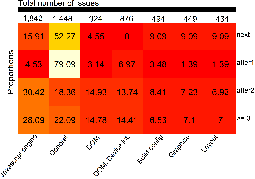
\includegraphics[width=0.60\textwidth,keepaspectratio]
	{chapters/chapter4/figures/firefox/RQ3_component_hm.pdf}
	\caption{\textbf{The spread of issues among the Firefox components.} The
		darker the colors, the smaller the proportion of issues that
	impact that component.}
	\label{ch4:fig:componentHeatmap}
\end{figure}

Furthermore, we study the distribution of addressed issues across components in the
Firefox project.
\hyperref[ch4:fig:componentHeatmap]{Figure}~\ref{ch4:fig:componentHeatmap} shows the top
seven components of the Firefox project, each having more than 400 addressed issues.
We analyze the proportion of addressed issues where \DIFdelbegin \DIFdel{integration }\DIFdelend \DIFaddbegin \DIFadd{delivery }\DIFaddend was prevented in the
top seven components.
\hyperref[ch4:fig:componentHeatmap]{Figure}~\ref{ch4:fig:componentHeatmap} shows that,
for buckets \textit{next} and \textit{after-1}, the majority of issues are
related to the \textit{General component}, whereas for \textit{after-2} and
\textit{after-3-or-more} the majority are related to the \textit{Javascript
engine} component. Addressed issues related to the \textit{General} component
may be easy to integrate, whereas issues related to the \textit{Javascript
Engine} may require more careful analysis before \DIFdelbegin \DIFdel{integration}\DIFdelend \DIFaddbegin \DIFadd{delivery}\DIFaddend .  \\


\noindent\DIFdelbegin \textit{\textbf{\DIFdel{Severity and priority have little influence on
delivery delay in terms of releases.}}%DIFAUXCMD
} %DIFAUXCMD
\DIFdelend \DIFaddbegin \finding{Severity and priority have little influence on
delivery delay in terms of releases.}{find11} \DIFaddend Users and contributors of software
projects can denote the importance of an issue using the \textit{priority} and
\textit{severity} fields. Previous studies have shown that priority and
severity have little influence on bug fixing time
\cite{tian2015unreliability,Herraiz2008,Mockus:2002}. For example, while an
issue might be severe or of high priority, it might be complex and would take a
long time to fix.  

However, in the integration context, we expect that priority and severity would
be more influential, since the issues have already been addressed. Even though
priority and severity are often left at their default values (see
\hyperref[ch4:sec:subjects]{Section}~\ref{ch4:sec:subjects}), one would expect that the
integrators would fast-track the integration of issues for which they
care about increasing the levels of severity or priority. For instance,
according to the Eclipse project guidelines for filing issue reports, a priority
level of P1 is used for serious issues and specifies that the existence of a P1
issue should prevent a release from
shipping.\smartfoot{\url{http://wiki.eclipse.org/Development_Resources/HOWTO/Bugzilla_Use}}
Hence, it is surprising that priority and severity play such a small role in
determining the release in which an addressed issue will appear. Indeed,
\hyperref[ch4:fig:variableImportance]{Figure}~\ref{ch4:fig:variableImportance} shows
that the priority and severity metrics obtain low importance scores.

\begin{figure}
	\centering
	%\captionsetup{justification=centering}
	\subfloat[ArgoUML Priority]{
		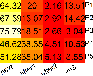
\includegraphics[width=0.30\textwidth,keepaspectratio] 
		{chapters/chapter4/figures/argouml/RQ3_priority_hm.pdf}
	\label{ch4:fig:heatMap_argo}}
	\subfloat[Eclipse Priority]{
		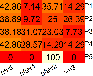
\includegraphics[width=0.30\textwidth,keepaspectratio] 
		{chapters/chapter4/figures/eclipse/RQ3_priority_hm.pdf}
	\label{ch4:fig:heatMap_eclipsep}}
	\subfloat[Firefox Priority]{
		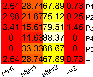
\includegraphics[width=0.30\textwidth,keepaspectratio]  
		{chapters/chapter4/figures/firefox/RQ3_priority_hm.pdf}
		\label{ch4:fig:heatMap_firefoxp}
	}

	\subfloat[Eclipse Severity]{
		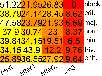
\includegraphics[width=0.35\textwidth,keepaspectratio] 
		{chapters/chapter4/figures/eclipse/RQ3_severity_hm.pdf}
	\label{ch4:fig:heatMap_eclipses}}
	\subfloat[Firefox Severity]{
		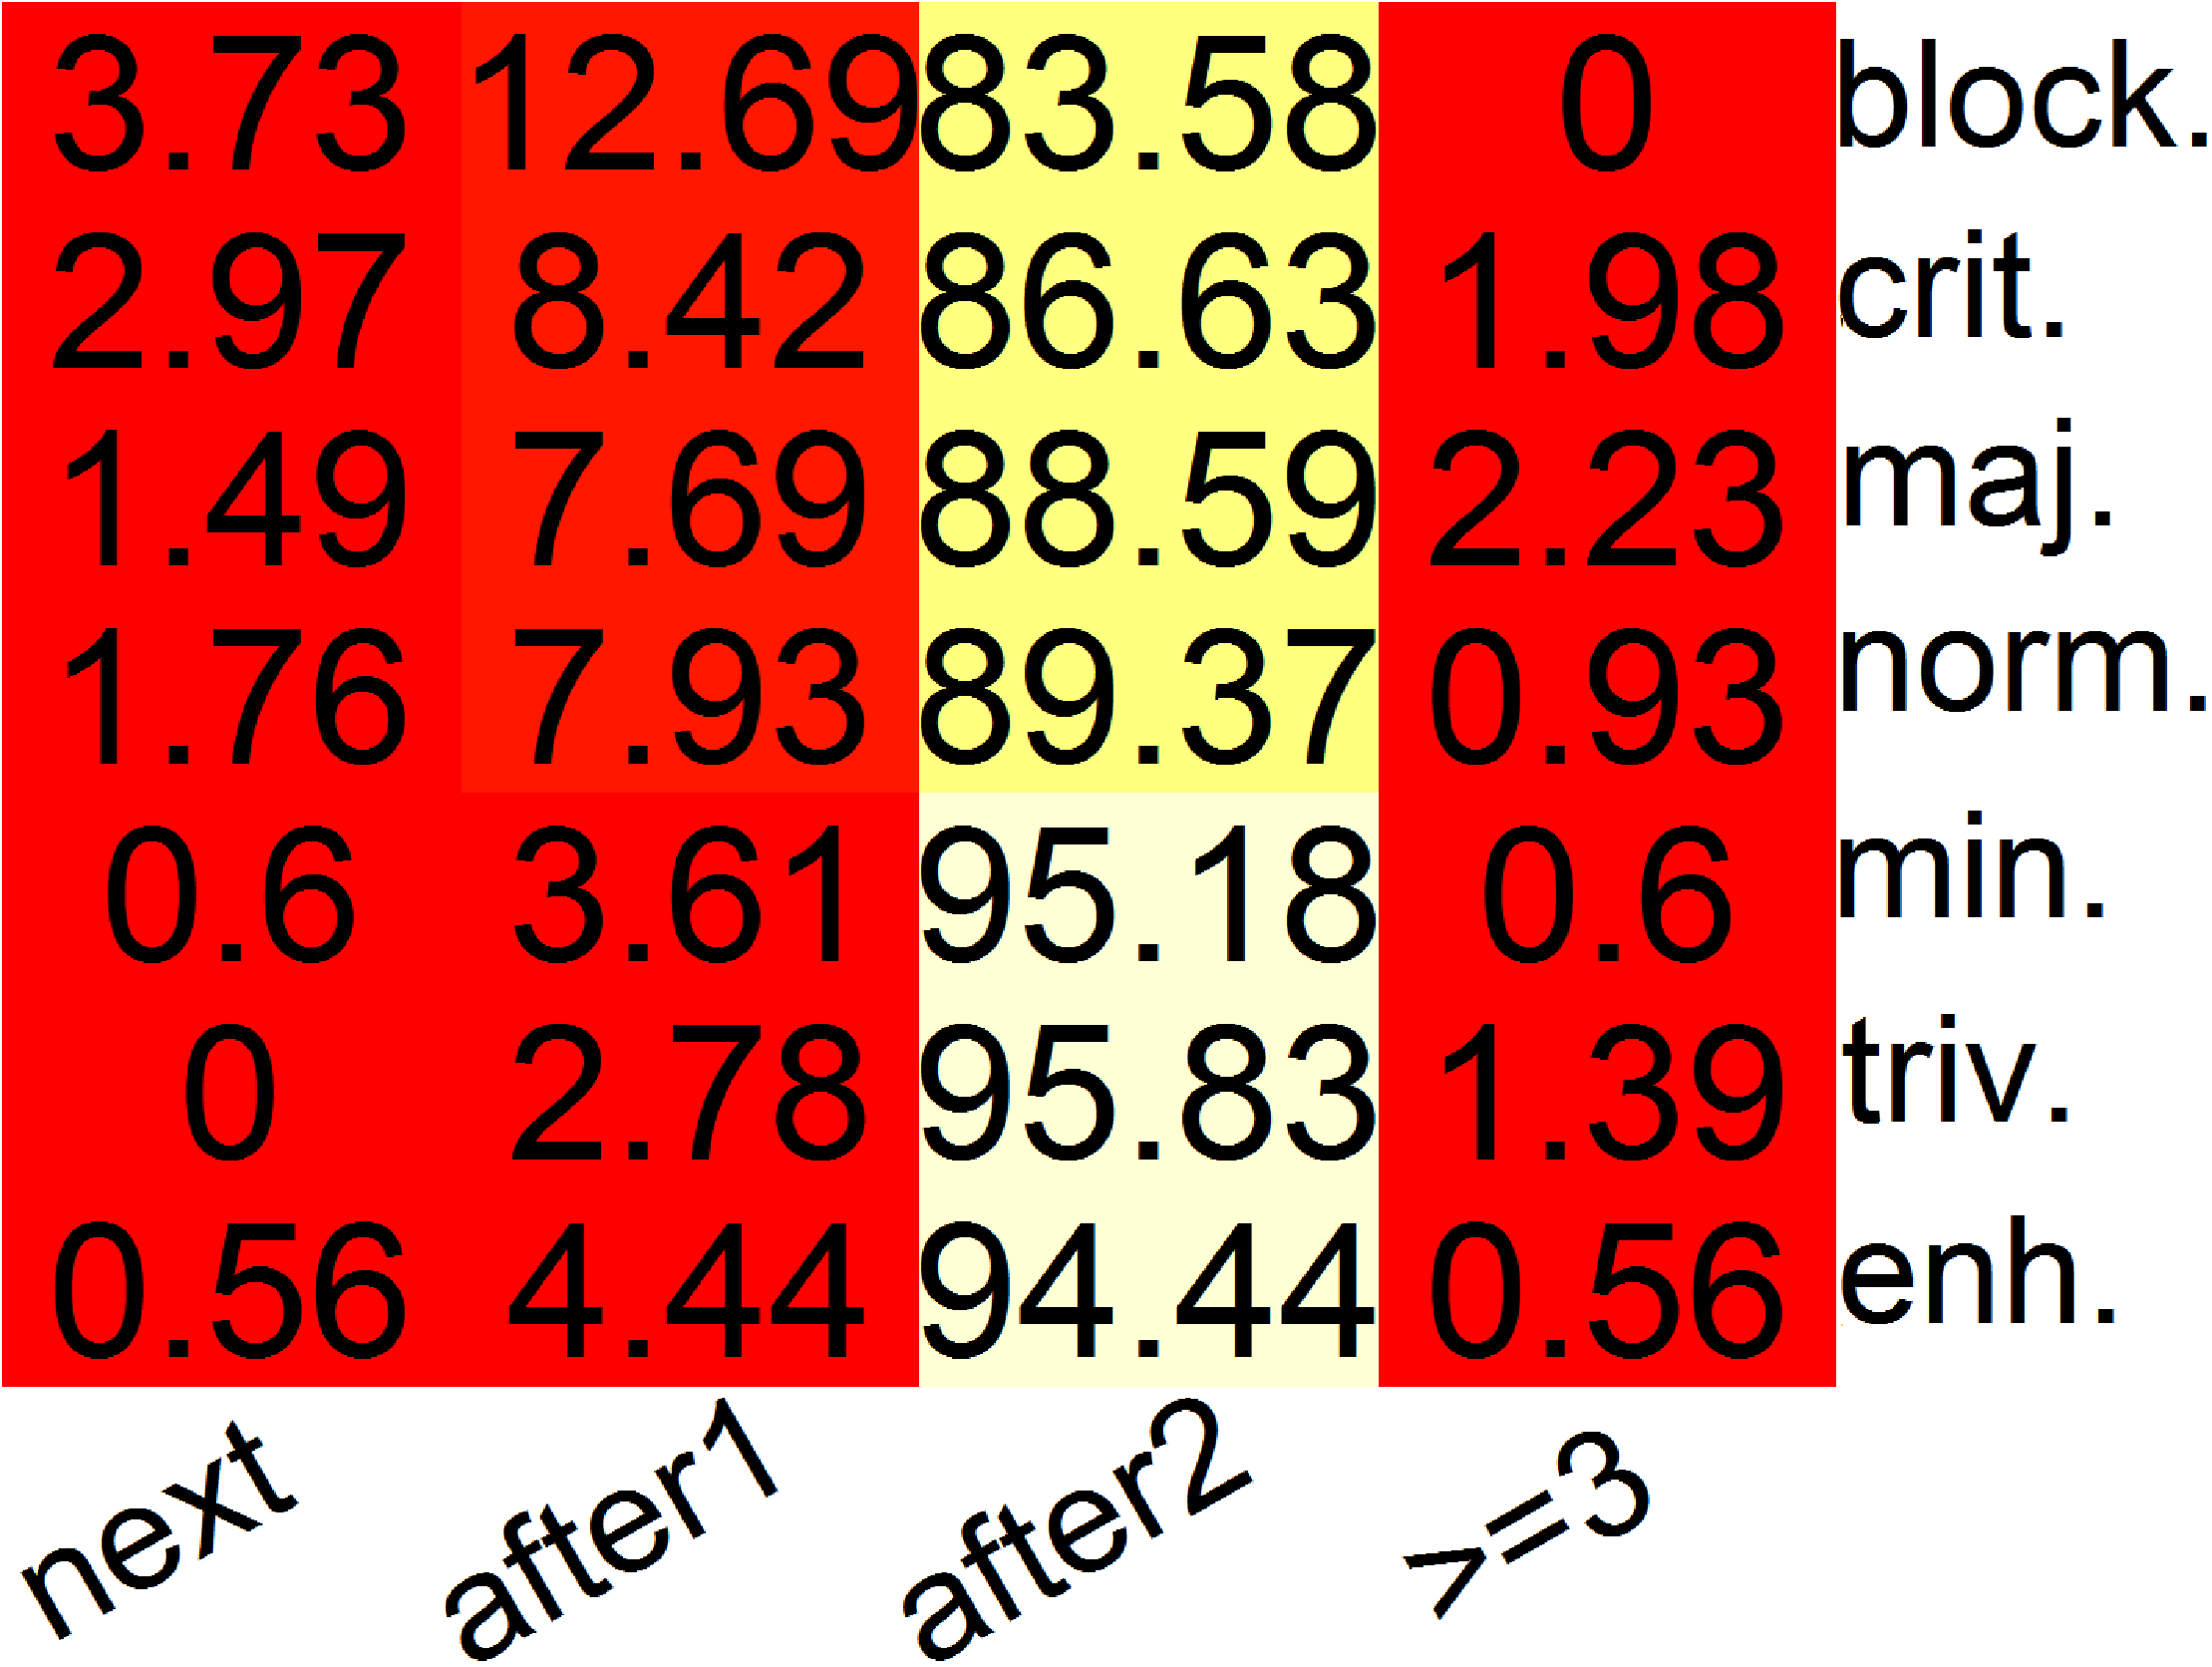
\includegraphics[width=0.35\textwidth,keepaspectratio]  
		{chapters/chapter4/figures/firefox/RQ3_severity_hm.pdf}
		\label{ch4:fig:heatMap_firefoxs}
	}
	\caption{\textbf{The percentage of priority and severity levels in each
		studied bucket of delivery delay.} We expect to see light
		colour in the upper left corner of these graphs, indicating that
		high priority/severity issues are \DIFdelbeginFL \DIFdelFL{integrated rapidly}\DIFdelendFL \DIFaddbeginFL \DIFaddFL{delivered quickly}\DIFaddendFL .
	Surprisingly, we are not seeing such a pattern in our datasets.}
	\label{ch4:fig:heatMaps}
\end{figure}

\hyperref[ch4:fig:heatMaps]{Figure}~\ref{ch4:fig:heatMaps} shows the percentage of
issues with a given priority (\textit{y-axis}) in a given \DIFdelbegin \DIFdel{integration }\DIFdelend \DIFaddbegin \DIFadd{delivery delay }\DIFaddend bucket
(\textit{x-axis}). The \DIFdelbegin \DIFdel{integration }\DIFdelend \DIFaddbegin \DIFadd{delivery }\DIFaddend of 36\% to 97\% of priority P1 addressed issues
had their \DIFdelbegin \DIFdel{integration }\DIFdelend \DIFaddbegin \DIFadd{delivery }\DIFaddend prevented in at least one release, whereas the \DIFdelbegin \DIFdel{integration
}\DIFdelend \DIFaddbegin \DIFadd{delivery
}\DIFaddend of 32\% to 96\% of priority P2 addressed issues were prevented from \DIFdelbegin \DIFdel{integration }\DIFdelend \DIFaddbegin \DIFadd{delivery }\DIFaddend in
at least one release. 

In the ArgoUML project, while the majority of priority P1 issues (64\%) were
\DIFdelbegin \DIFdel{integrated }\DIFdelend \DIFaddbegin \DIFadd{delivered }\DIFaddend in the \textit{next} release, 36\% of them had their \DIFdelbegin \DIFdel{integration
}\DIFdelend \DIFaddbegin \DIFadd{delivery
}\DIFaddend prevented in at least one release. For the Firefox project, 97\% of the P1
issues and 96\% of the \textit{blocker} issues were prevented from \DIFdelbegin \DIFdel{integration
}\DIFdelend \DIFaddbegin \DIFadd{delivery
}\DIFaddend in at least one release. Finally, for the Eclipse project, 57\% of P1 issues and
49\% of blocker issues had their \DIFdelbegin \DIFdel{integration }\DIFdelend \DIFaddbegin \DIFadd{delivery }\DIFaddend prevented in at least one release.
Hence, our data shows that, in the context of issue \DIFdelbegin \DIFdel{integration}\DIFdelend \DIFaddbegin \DIFadd{delivery}\DIFaddend , the
\textit{priority} and \textit{severity} values that are recorded in the ITSs
have little influence on delivery delay. Instead, addressed issues might be
prioritized by the level of risk that are associated to them.\DIFdelbegin %DIFDELCMD < \smartfoot{Two issues from our sample were
%DIFDELCMD < 	promoted to stabler release channels due to low associated risk \url{https://bugzilla.mozilla.org/show_bug.cgi?id=724145} and
%DIFDELCMD < \url{https://bugzilla.mozilla.org/show_bug.cgi?id=732962}, while another issue was prevented from integration due to code break
%DIFDELCMD < \url{https://bugzilla.mozilla.org/show_bug.cgi?id=723793}.} %%%
\DIFdelend \DIFaddbegin \smartfoot{Two
	issues from our sample were promoted to stabler release channels due to
	low associated risk
	\url{https://bugzilla.mozilla.org/show_bug.cgi?id=724145} and
	\url{https://bugzilla.mozilla.org/show_bug.cgi?id=732962}, while another
	issue was prevented from delivery due to code break
\url{https://bugzilla.mozilla.org/show_bug.cgi?id=723793}.} \DIFaddend This might explain
why the time that is invested on fixing issues during a release cycle reduces
delivery delay---a risk of an addressed issue breaking the code would be smaller
when more time is invested at fixing activities. 

\conclusionbox{The total time that is invested in fixing issues of a release
	cycle and integration workload attributes are the most influential
	attributes in our models. We also find that priority and severity have
	little influence in estimating delivery delay.}

\subsubsection*{\textbf{\textit{RQ4: Results for delivery delay in terms of days}}}

\begin{table}[t]
	\scriptsize
	\centering
	\caption{\textbf{Explanatory power of attributes.} We present the
		$\chi^2$ proportion and the degrees of freedom that are spent
		for each attribute. The $\chi^2$ of the two most influential
		attributes of each model are in bold.
	\label{ch4:tbl:explanatory_power}}
	\begin{threeparttable}
		\begin{tabular}{llrrr}
			\cline{3-5} 
			\multicolumn{2}{c}{} & 
			Eclipse &
			Firefox &
			ArgoUML
			\tabularnewline
			\hline
			\multicolumn{2}{l}{Wald $\chi^2$} & 
			$1,180$ &
			$8,560$ &
			$2,803$
			\tabularnewline
			\hline 
			\multicolumn{2}{l}{Budgeted Degrees of Freedom} &
			$87$ & 
			$879$ &
			$102$
			\tabularnewline
			\hline
			\multicolumn{2}{l}{Degrees of Freedom Spent} &
			$24$ & 
			$33$ &
			$28$
			\tabularnewline
			\hline 
			\multirow{2}{*}{Reporter experience} & 
			D.F. & 
			$1$ & 
			$1$ &
			$1$
			\tabularnewline 
			& 
			$\chi^2$ & 
			$4^{\ast\ast\ast}$ &  
			$\approx 0$ &
			$1^{\ast\ast}$
			\tabularnewline
			\hline 
			\multirow{2}{*}{Resolver experience} & 
			D.F. & 
			$1$ & 
			$1$ &
			$1$
			\tabularnewline 
			& 
			$\chi^2$ & 
			$12^{\ast\ast\ast}$ & 
			$\approx 0^{\ast}$ &  
			$\approx 0$ 
			\tabularnewline
			\hline 
			\multirow{2}{*}{Reporter integration speed} & 
			D.F. & 
			$3$ & 
			$1$ &
			$2$
			\tabularnewline &
			$\chi^2$ & 
			$16^{\ast\ast\ast}$ &
			$\approx 0$ &
			$1^{\ast}$
			\tabularnewline  
			\hline 
			\multirow{2}{*}{Resolver integration speed} & 
			D.F. & 
			$2$ & 
			$1$ &
			$4$
			\tabularnewline & 
			$\chi^2$ & 
			$\mathbf{22}^{\ast\ast\ast}$ &
			$\approx 0$ &  
			$\mathbf{9}^{\ast\ast\ast}$
			\tabularnewline
			\hline 
			\multirow{2}{*}{Fixing time} & 
			D.F. & 
			$2$ & 
			\multirow{2}{*}{$\oplus$} &
			$1$
			\tabularnewline & 
			$\chi^2$ & 
			$1^{\ast}$ &
			&  
			$1^{\ast\ast}$ 
			\tabularnewline
			\hline 
			\multirow{2}{*}{Severity} & 
			D.F. & 
			$6$ &
			$6$ &
			\multirow{2}{*}{$\ominus$} 
			\tabularnewline & 
			$\chi^2$ &
			$\approx 0$ &
			$8^{\ast\ast\ast}$ &
			%\ominus
			\tabularnewline \hline 
			\multirow{2}{*}{Priority} &
			D.F. & 
			\multirow{2}{*}{$\oslash$} & 
			$5$ &
			$5$
			\tabularnewline & 
			$\chi^2$ & 
			&%\oslash
			$5^{\ast\ast\ast}$ &  
			$1^{\ast}$  
			\tabularnewline \hline 
			\multirow{2}{*}{Description size} & 
			D.F. & 
			$1$ & 
			$1$ &
			$1$
			\tabularnewline & 
			$\chi^2$ & 
			$\approx 0$ &  
			$\approx 0$ &
			$\approx 0$
			\tabularnewline \hline 
			\multirow{2}{*}{Impacted files} & 
			D.F. & 
			$1$ &
			$1$ &
			$1$
			\tabularnewline & 
			$\chi^2$ & 
			$\approx 0$ &
			$\approx 0^{\ast\ast}$ &
			$\approx $
			\tabularnewline \hline 
			\multirow{2}{*}{Number of comments} & 
			D.F. & 
			$1$ &
			$1$ &  
			$1$
			\tabularnewline & 
			$\chi^2$ & 
			$2^{\ast\ast}$ &  
			$1^{\ast\ast\ast}$  &
			$\approx 0$
			\tabularnewline \hline 
			\multirow{2}{*}{Reassignments} & 
			D.F. & 
			$1$ & 
			$1$ &
			$1$
			\tabularnewline & 
			$\chi^2$ & 
			$\approx 0$ &  
			$\approx 0$ &
			$1^{\ast}$
			\tabularnewline \hline 
			\multirow{2}{*}{Number of activities} & 
			D.F. & 
			$1$ &
			$1$ &
			$1$
			\tabularnewline & 
			$\chi^2$ & 
			$\approx 0$ &  
			$\approx 0$ &
			$\approx 0$
			\tabularnewline \hline 
			\multirow{2}{*}{Interval between comments} & 
			D.F. & 
			$1$ &
			$1$ &
			\multirow{2}{*}{$\oslash$}
			\tabularnewline & 
			$\chi^2$ & 
			$1^{\ast}$ &  
			$\approx 0$ &
			%\oslash correlation
			\tabularnewline \hline 
			\multirow{2}{*}{Churn} & 
			D.F. & 
			$1$ &
			$1$ &
			$1$
			\tabularnewline & 
			$\chi^2$ & 
			$\approx 0$ &  
			$\approx 0$ &
			$1^{\ast\ast}$
			\tabularnewline \hline 
			\multirow{2}{*}{Number of concurrent issues} & 
			D.F. & 
			\multirow{2}{*}{$\oslash$} &
			$2$ &
			\multirow{2}{*}{$\oslash$}
			\tabularnewline &
			$\chi^2$ &
			& %\oslash
			$\mathbf{8}^{\ast\ast\ast}$ &
			%\oslash
			\tabularnewline \hline 
			\multirow{2}{*}{Number of concurrent issues per resolver} & 
			D.F. & 
			$1$ & 
			$2$ &
			$2$
			\tabularnewline &
			$\chi^2$ &
			$7^{\ast\ast\ast}$ &  
			$2^{\ast\ast\ast}$ &
			$\mathbf{9}^{\ast\ast\ast}$
			\tabularnewline \hline 
			\multirow{2}{*}{Queue position} & 
			D.F. & 
			$1$ &             
			$4$ &
			$2$
			\tabularnewline & 
			$\chi^2$ & 
			$\mathbf{23}^{\ast\ast\ast}$ & 
			$\mathbf{83}^{\ast\ast\ast}$ &
			$\mathbf{67}^{\ast\ast\ast}$
			\tabularnewline \hline 
			\multirow{1}{*}{Fixing time per resolver} & 
			D.F. & 
			$1$ & 
			$2$ &
			$4$
			\tabularnewline &
			$\chi^2$ & 
			$7^{\ast\ast\ast}$ & 
			$\approx 0^{\ast\ast}$ &
			$8^{\ast\ast\ast}$
			\tabularnewline \hline 
		\end{tabular}
		\begin{tablenotes}
		\item[$\oslash$] Discarded during correlation analysis 
		\item[$\oplus$] Discarded during redundancy analysis 
		\item[$\ominus$] The variable does not apply to the dataset
		\item[$\ast$] $p < 0.05$
		\item[$\ast\ast$] $p < 0.01$
		\item[$\ast\ast\ast$] $p < 0.001$ 
		\end{tablenotes}
	\end{threeparttable}
\end{table}

\noindent\DIFdelbegin \textbf{\textit{\DIFdel{Project family attributes, such as the backlog of
issues and queue position provide most of the explanatory power of our models.}}%DIFAUXCMD
}
%DIFAUXCMD
\DIFdelend \DIFaddbegin \finding{Project family attributes, such as the backlog of
issues and queue position provide most of the explanatory power of our
models.}{find12}
\DIFaddend \hyperref[ch4:tbl:explanatory_power]{Table}~\ref{ch4:tbl:explanatory_power} shows the
explanatory power of each of the attributes of our models. The two most
influential attributes for each model are shown in bold. \textit{Queue
position}, \ie the time at which an issue is addressed is the most influential
attribute in all of the models that are fitted to our studied projects.
Interestingly, we observe that \textit{resolver integration speed}---the median
delivery delay of the previously resolved issues of a particular
resolver---plays an influential role in our models that are fit for the Eclipse
and ArgoUML projects. Moreover, we also observe that integration workload
attributes (\ie \textit{backlog of issues}, and \textit{backlog of issues per
resolver}) are very influential in our models that are fit for the Firefox and
ArgoUML projects.\\

\begin{figure}
	\centering
	\subfloat[Eclipse]{
		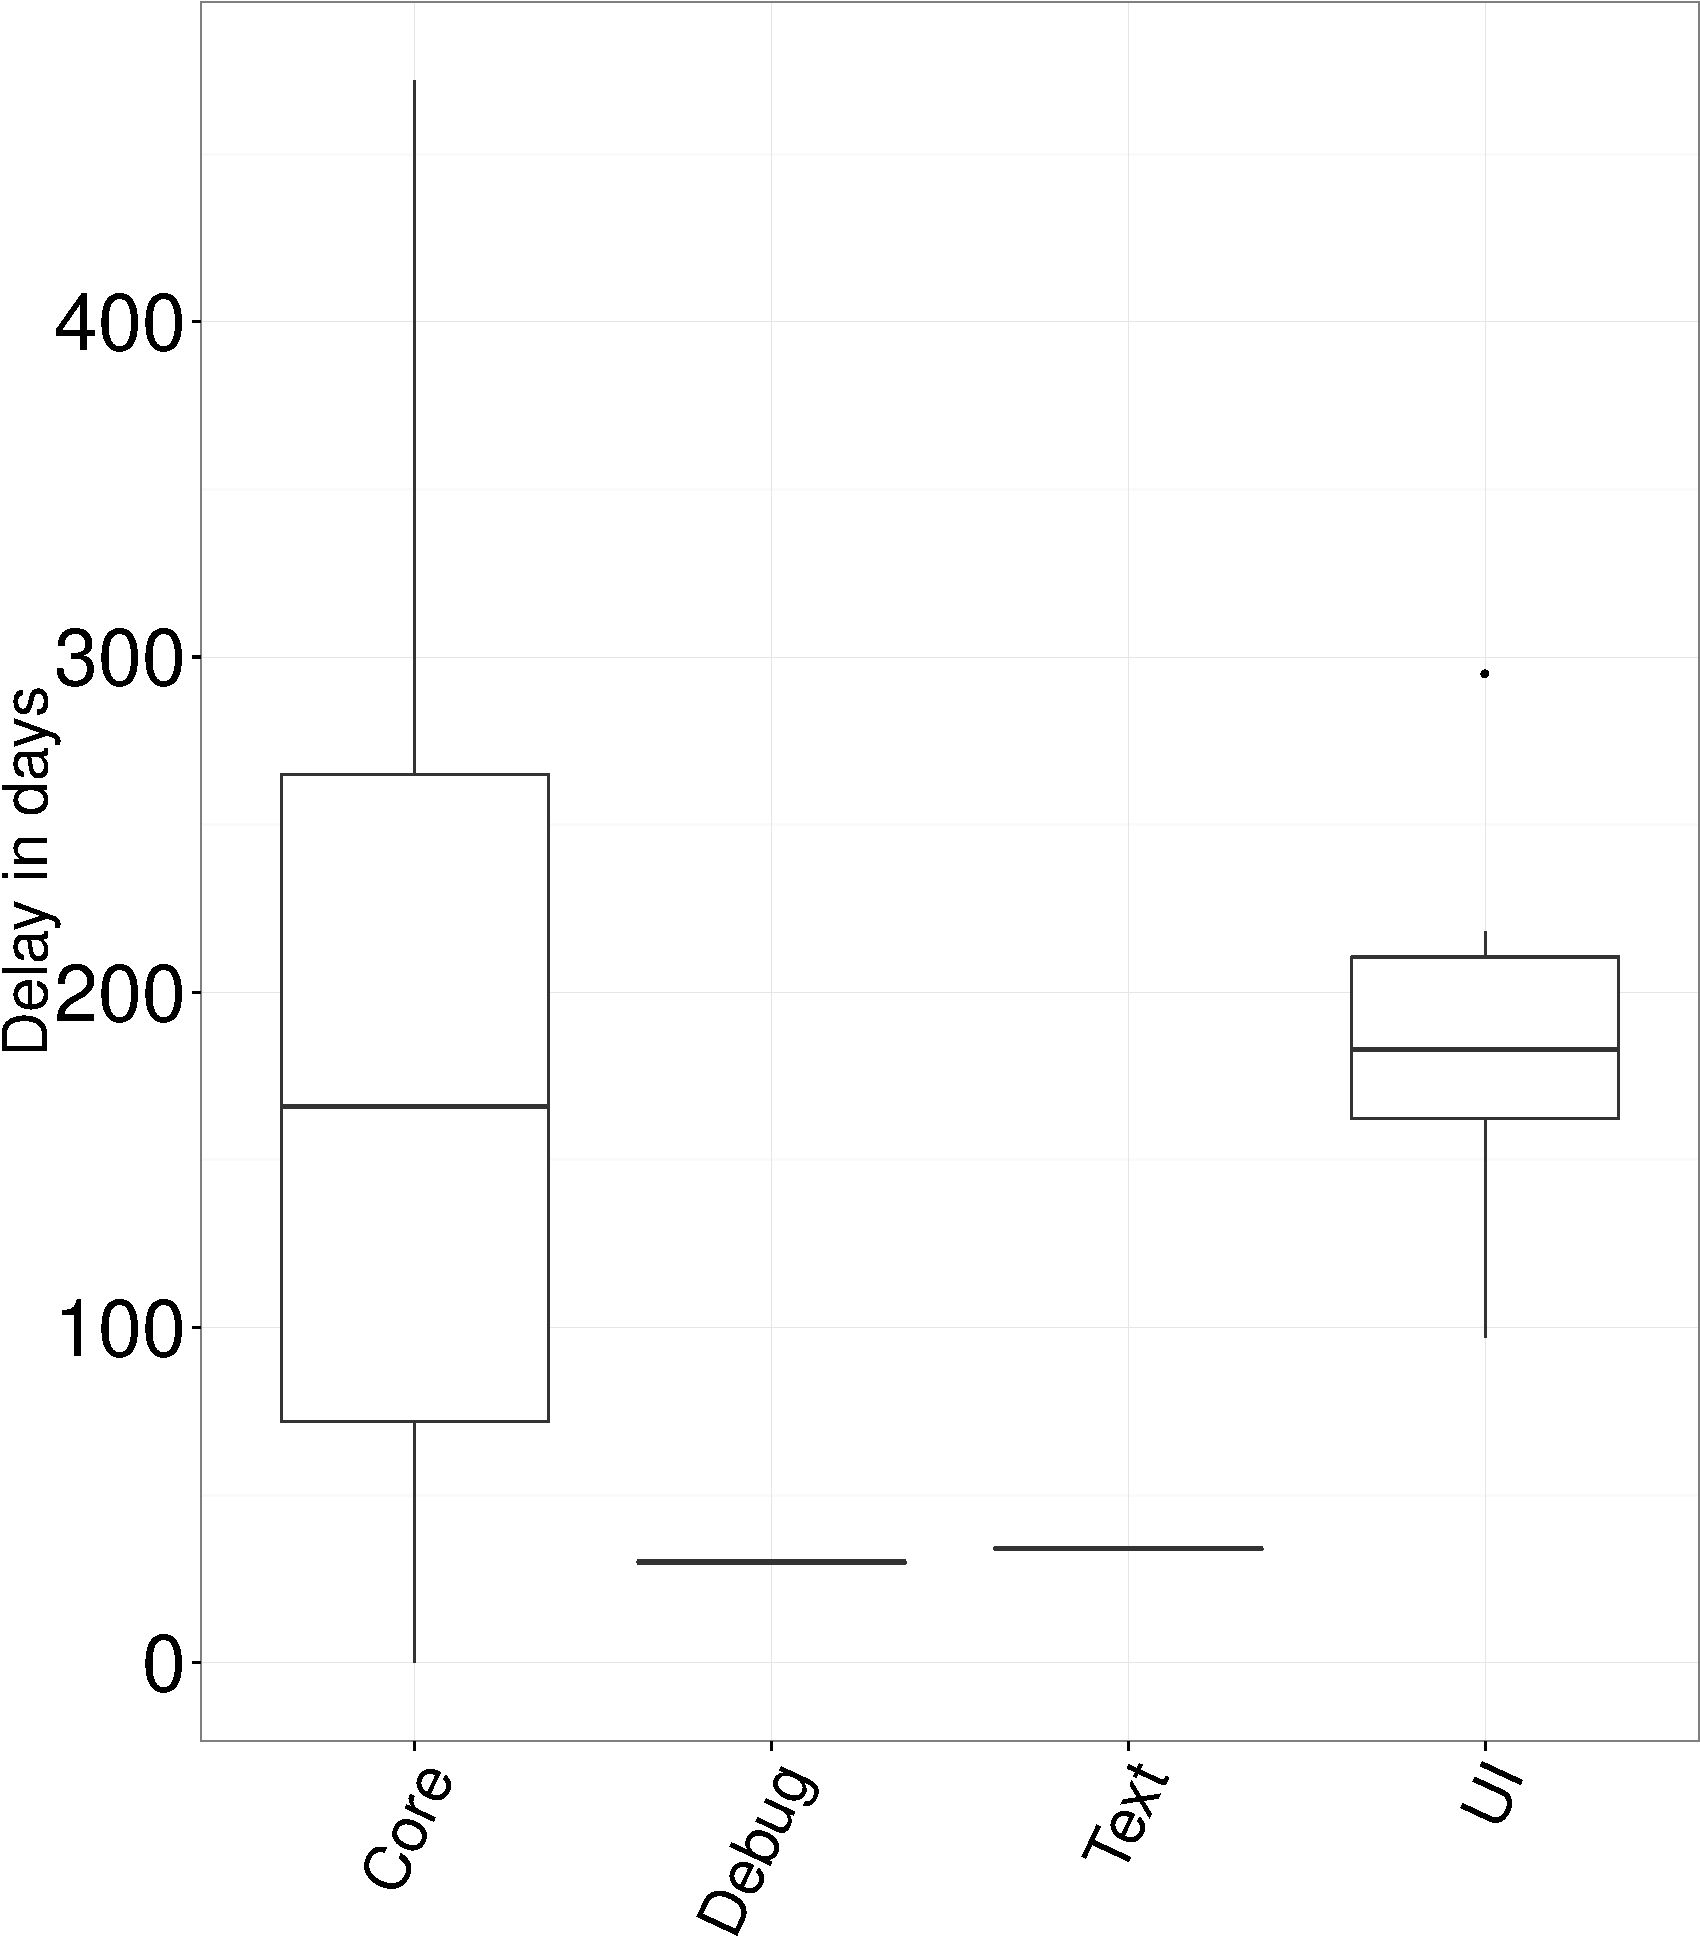
\includegraphics[width=0.40\textwidth,keepaspectratio]
		{chapters/chapter4/figures/components_eclipse.pdf}
	}

	\subfloat[Firefox]{
		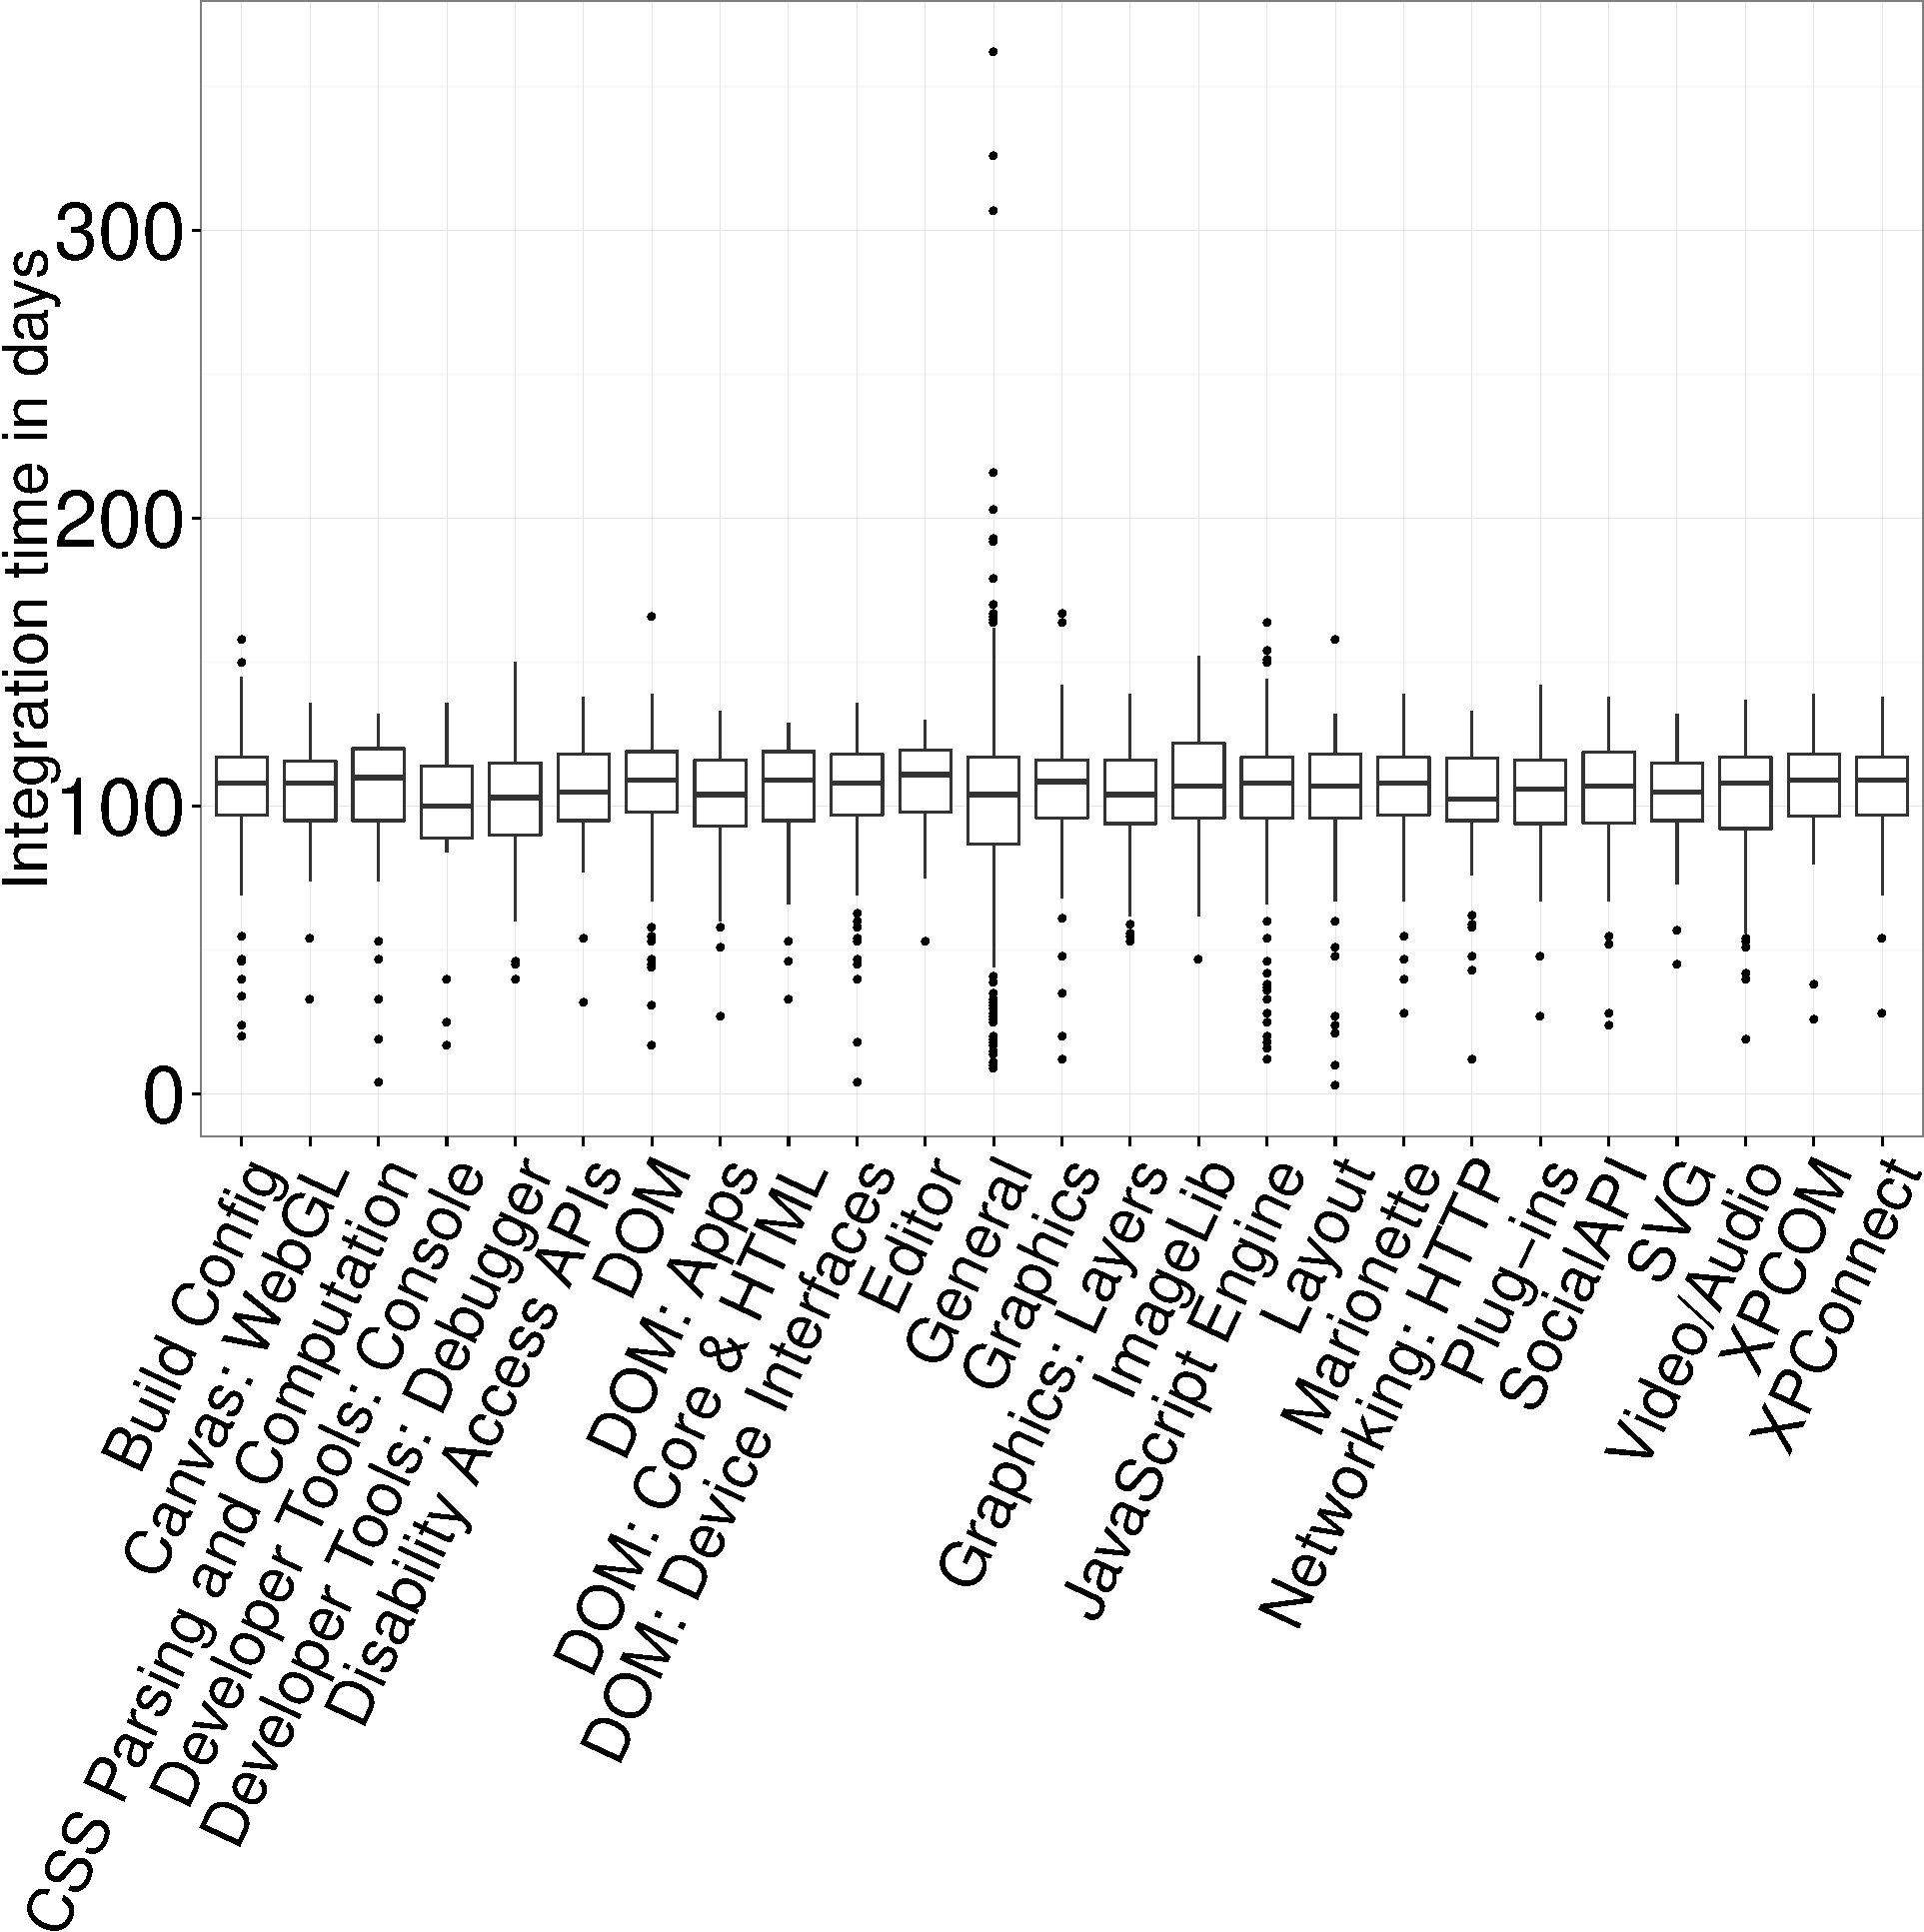
\includegraphics[width=0.40\textwidth,keepaspectratio]
		{chapters/chapter4/figures/components_firefox.pdf}
	}

	\subfloat[ArgoUML]{
		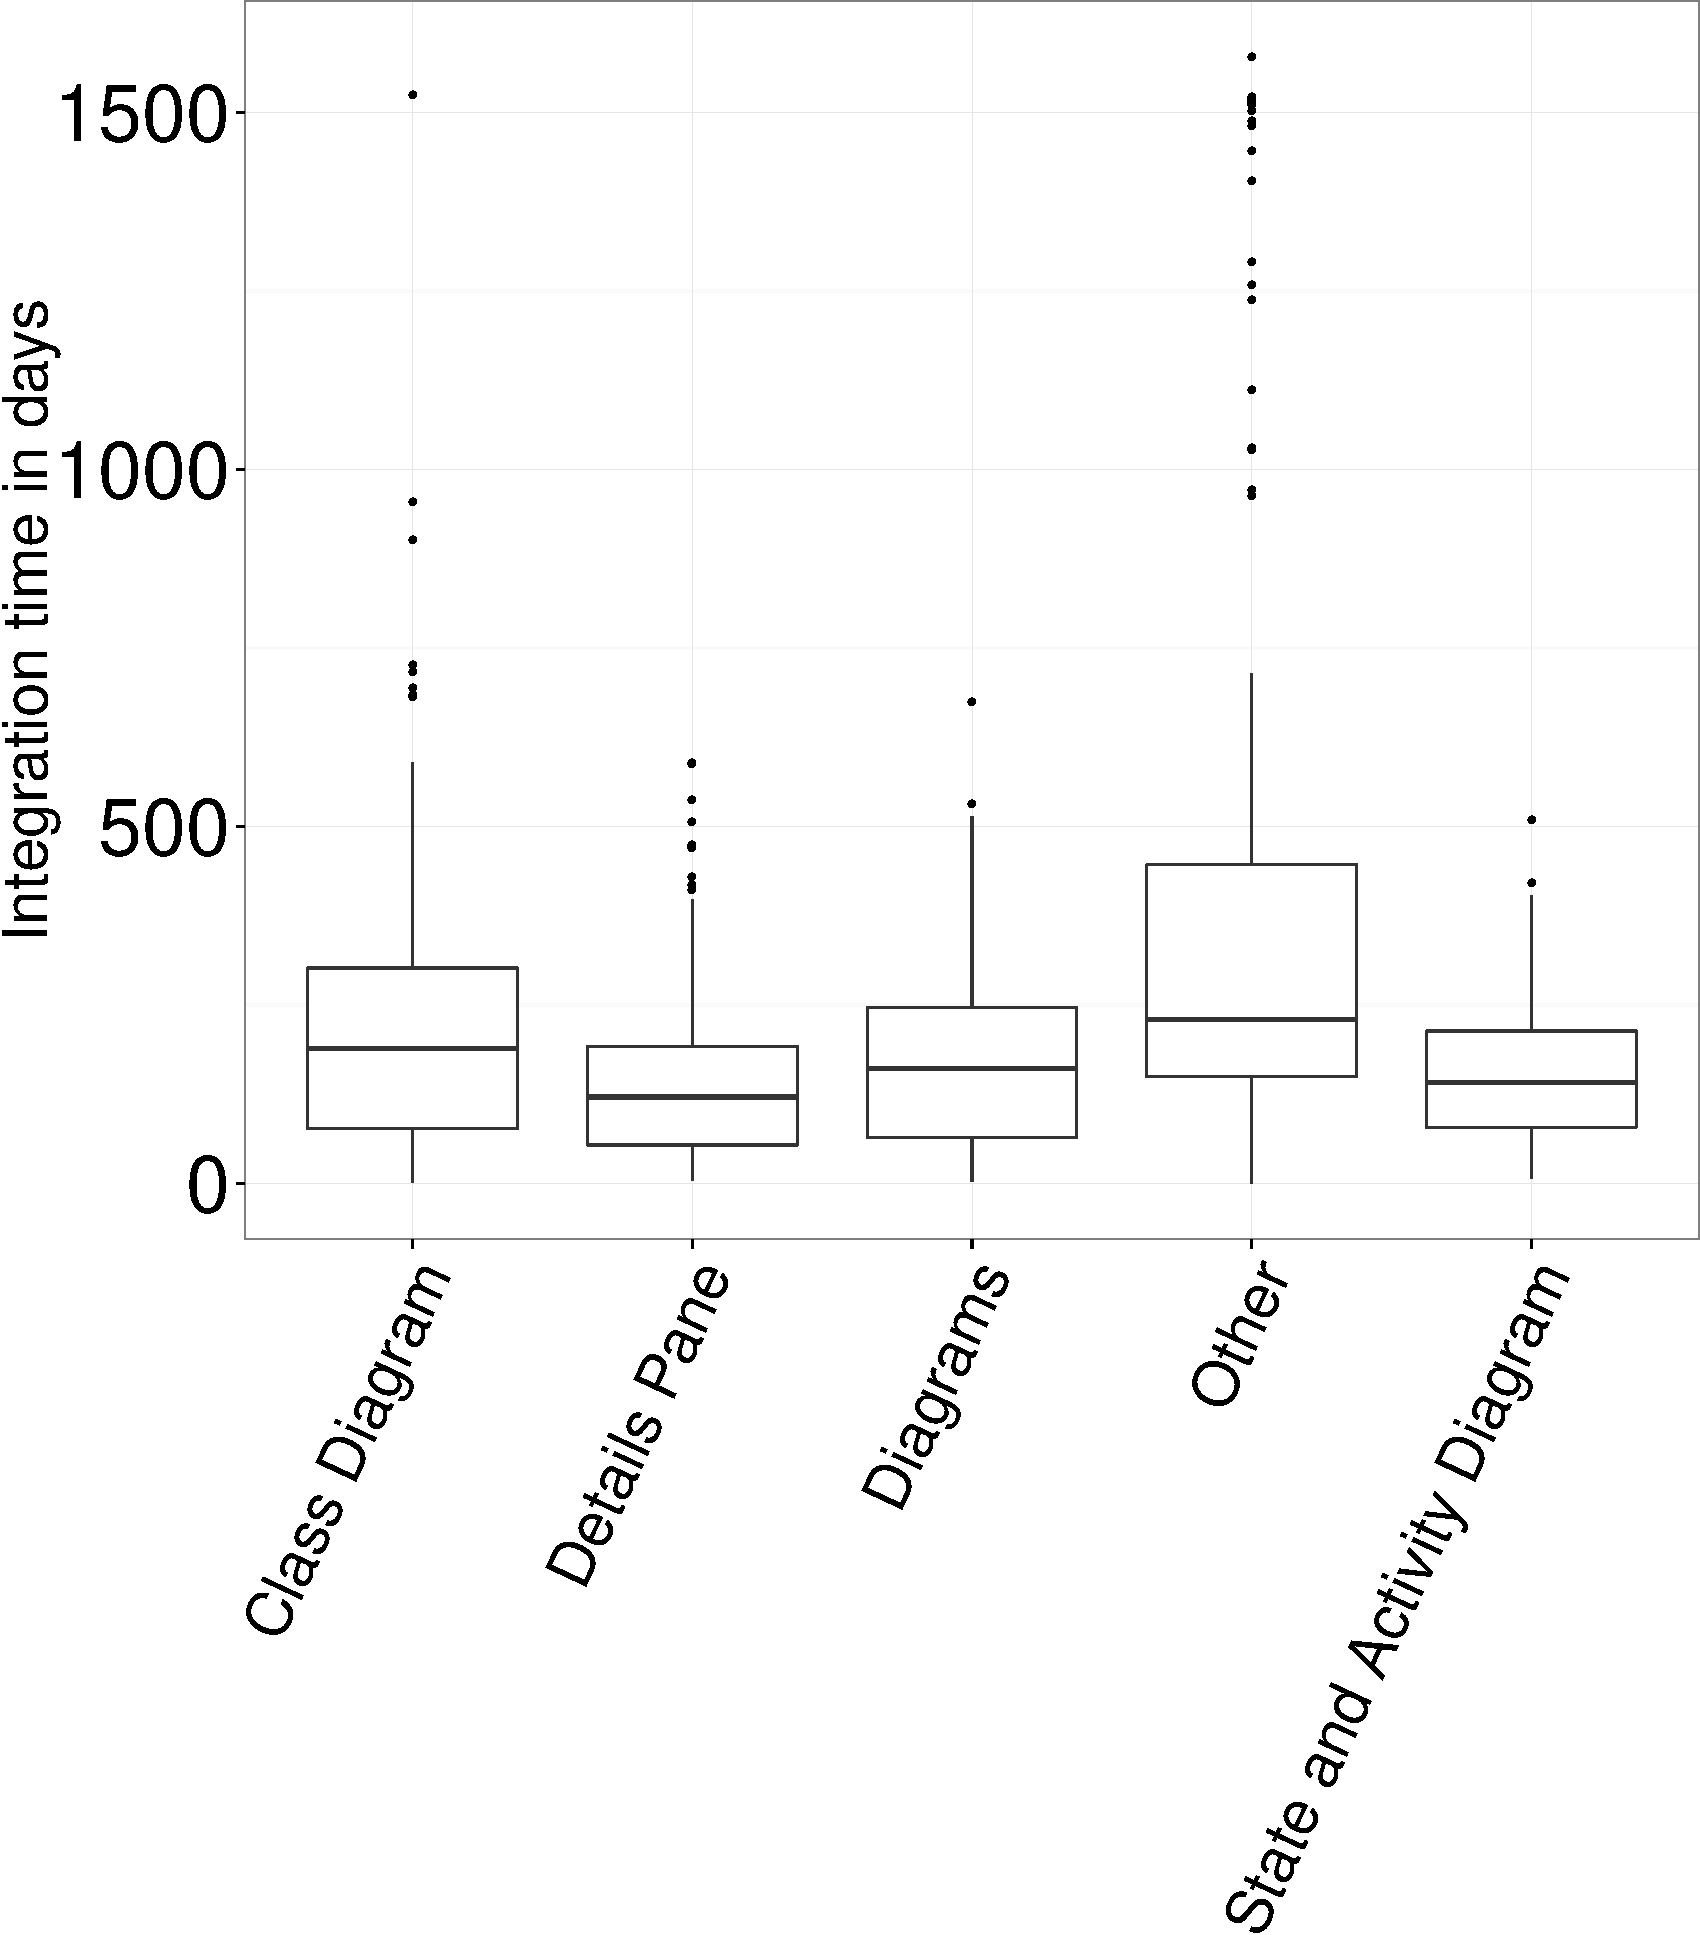
\includegraphics[width=0.40\textwidth,keepaspectratio]
		{chapters/chapter4/figures/components_argouml.pdf}
	}
	\caption{\textbf{Delivery delay per component.} The Figure shows the
		distributions of delivery delay in terms of days for each
		component of the studied projects.
	}
	\label{ch4:fig:component_analysis}
\end{figure}

\noindent\DIFdelbegin \textbf{\textit{\DIFdel{The component to which an issue is addressed has little
impact in the delivery delay in terms of days.}}%DIFAUXCMD
} %DIFAUXCMD
\DIFdelend \DIFaddbegin \finding{The component to which an issue is addressed has little
impact in the delivery delay in terms of days.}{find13} \DIFaddend To demonstrate this, we group
each addressed issue according to the components that such an issue modifies. We use
components that have at least 100 addressed issues as a threshold for our analysis.
We then compare the distribution of delivery delay in terms of days in these
components.
\hyperref[ch4:fig:component_analysis]{Figure}~\ref{ch4:fig:component_analysis} shows the
distributions of delivery delay in terms of days per component. We do not
observe a considerable difference between distributions of delivery delay in
the ArgoUML or Firefox projects. The distribution of the ``Other'' component in
the ArgoUML project is more skewed, which is suggestive of its generic
role---such a component may encompass a more broad spectrum of addressed issues. On
the other hand, 99\% of the addressed issues in the Eclipse (JDT) project belong to
the ``Core'' component (thus its skewness). Finally, the ``Debug'' and ``Text''
Eclipse components contain only one addressed issue each.   

\conclusionbox{The workload in terms of backlog of issues awaiting integration
	and the integration speed of prior addressed issues of a given resolver play
	a important role to model delivery delay in terms of days. Moreover,
	the initial \textit{queue position} is the most important attribute in
	all models that we fit to study delivery delay in terms of days.}

\subsection{RQ5: How well can we identify the addressed issues
that will suffer from a prolonged delivery delay?}\label{ch4:rq5}

\subsubsection*{RQ5: Motivation} 

End users may get frustrated if an addressed issue that s/he is interested has a
prolonged delivery delay. Furthermore, if such a delivery delay is unexpected for a
particular system (\eg it is very long), the frustration of users may increase
considerably, since they are not used to such a \DIFdelbegin \DIFdel{integration time}\DIFdelend \DIFaddbegin \DIFadd{delivery delay}\DIFaddend . In
\hyperref[ch4:rq5]{RQ5} we
investigate if we can accurately identify which addressed issues are likely to
have a prolonged delivery delay. This investigation helps us mitigate the problem of
prolonged delivery delay of addressed issues.

\subsubsection*{RQ5: Approach} We calculate prolonged delivery delay
(\hyperref[def:3]{Definition}~\ref{def:3}) as
described in the \hyperref[settings:step3]{Step 3} of our data collection
process. Indeed, in
\hyperref[ch4:fig:beanplot_days]{Figure}~\ref{ch4:fig:beanplot_days}, we observe that
the distribution of delivery delay of the Eclipse and ArgoUML projects have more variation than
the distribution of the Firefox project.

The hexbin plots of \hyperref[ch4:fig:hexbins]{Figure}~\ref{ch4:fig:hexbins} show the
relationship between the delivery delay in terms of releases and days. Hexbin
plots are scatterplots that represent several data points with hexagon-shaped
bins. The lighter the shade of the hexagon, the more data points that fall
within the bin. Indeed, \hyperref[ch4:fig:hexbins]{Figure}~\ref{ch4:fig:hexbins}
suggests that the longer the delivery delay in terms of days, the longer is
the delivery delay in terms of releases. This tendency is more clear in the
Eclipse and Firefox projects. On the other hand, in the ArgoUML project, we
observe addressed issues with a longer delivery delay in terms of releases but
with a shorter delivery delay in terms of days. For instance, we observe addressed
issues with a delivery delay of four releases that have a shorter \DIFdelbegin \DIFdel{integration
time }\DIFdelend \DIFaddbegin \DIFadd{delivery
delay }\DIFaddend in terms of days than addressed issues with a delivery delay of three
releases.  Such behaviour in the ArgoUML project may be explained by the skew in
the distance between the releases of this project ({\em cf.}
\hyperref[ch4:fig:releaseIntervals]{Figure}~\ref{ch4:fig:releaseIntervals}).

\begin{figure}[t]
	\centering
	\subfloat[Eclipse]{
		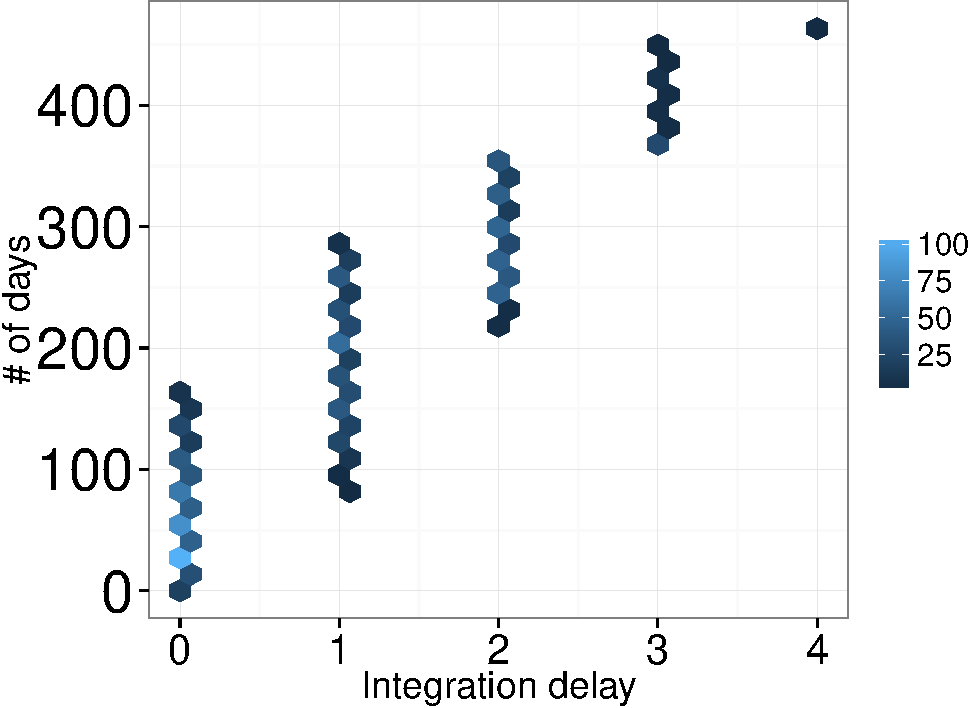
\includegraphics[width=0.49\textwidth,keepaspectratio]
		{chapters/chapter4/figures/eclipse_hexbinplot.pdf}
		\label{ch4:fig:eclipse_hexbin}
	}
	\subfloat[Firefox]{
		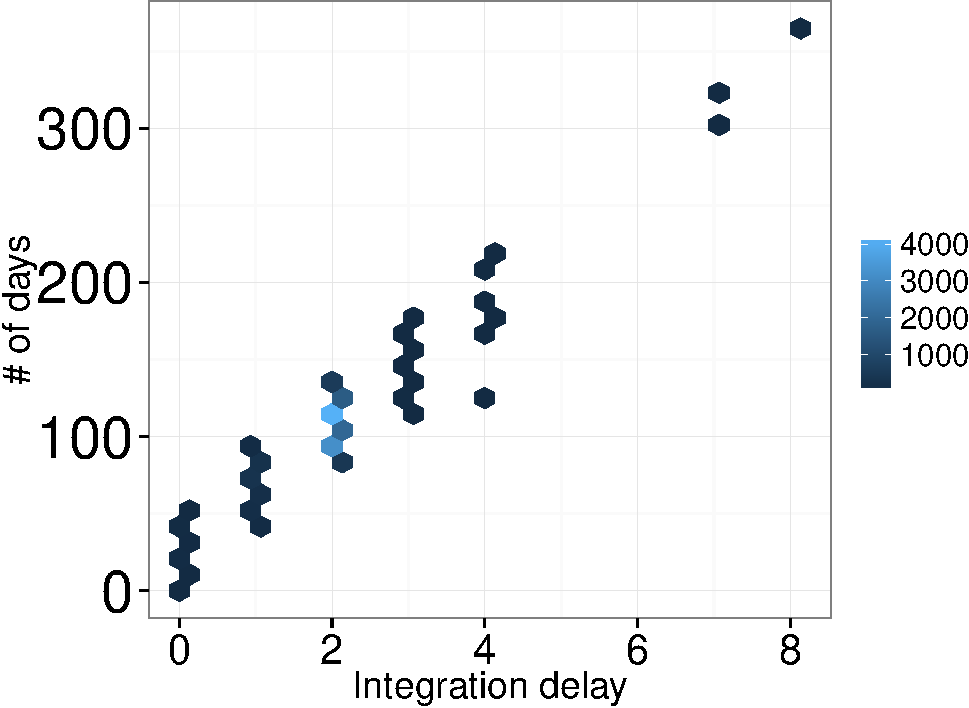
\includegraphics[width=0.49\textwidth,keepaspectratio]
		{chapters/chapter4/figures/firefox_hexbinplot.pdf}
		\label{ch4:fig:firefox_hexbin}
	}

	\subfloat[ArgoUML]{
		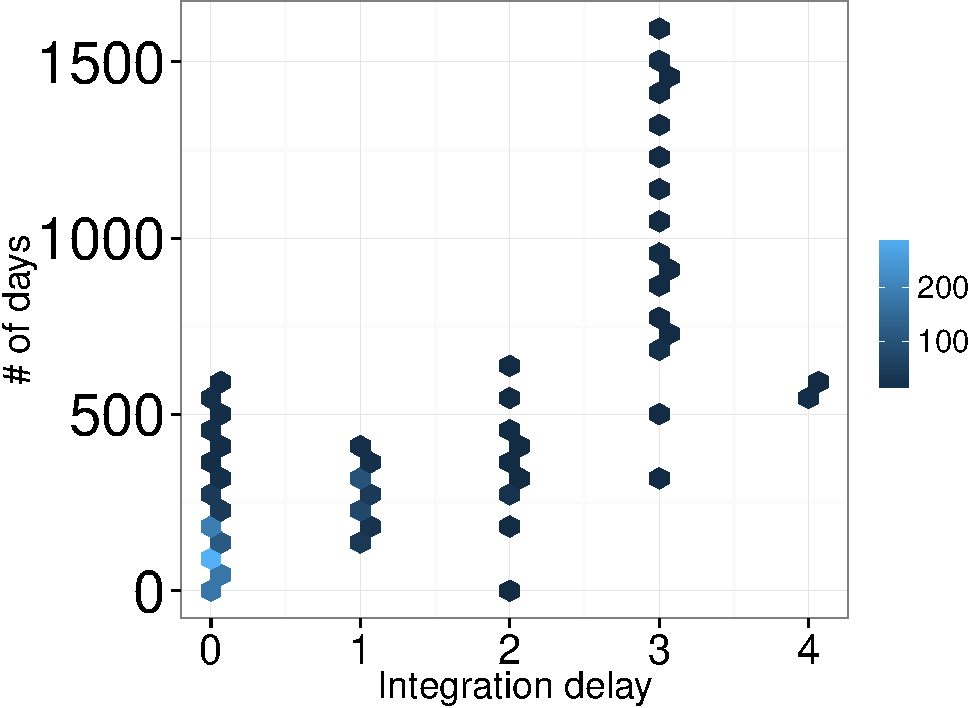
\includegraphics[width=0.49\textwidth,keepaspectratio]
		{chapters/chapter4/figures/argouml_hexbinplot.pdf}
		\label{ch4:fig:argouml_hexbin}
	}
	\caption{\textbf{Relationship between delivery delay in terms of
		releases and days.} We observe that
		a longer delivery delay in terms of releases is associated with a
	longer delivery delay in terms of days.}
	\label{ch4:fig:hexbins}
\end{figure}

\begin{figure}
	\centering
	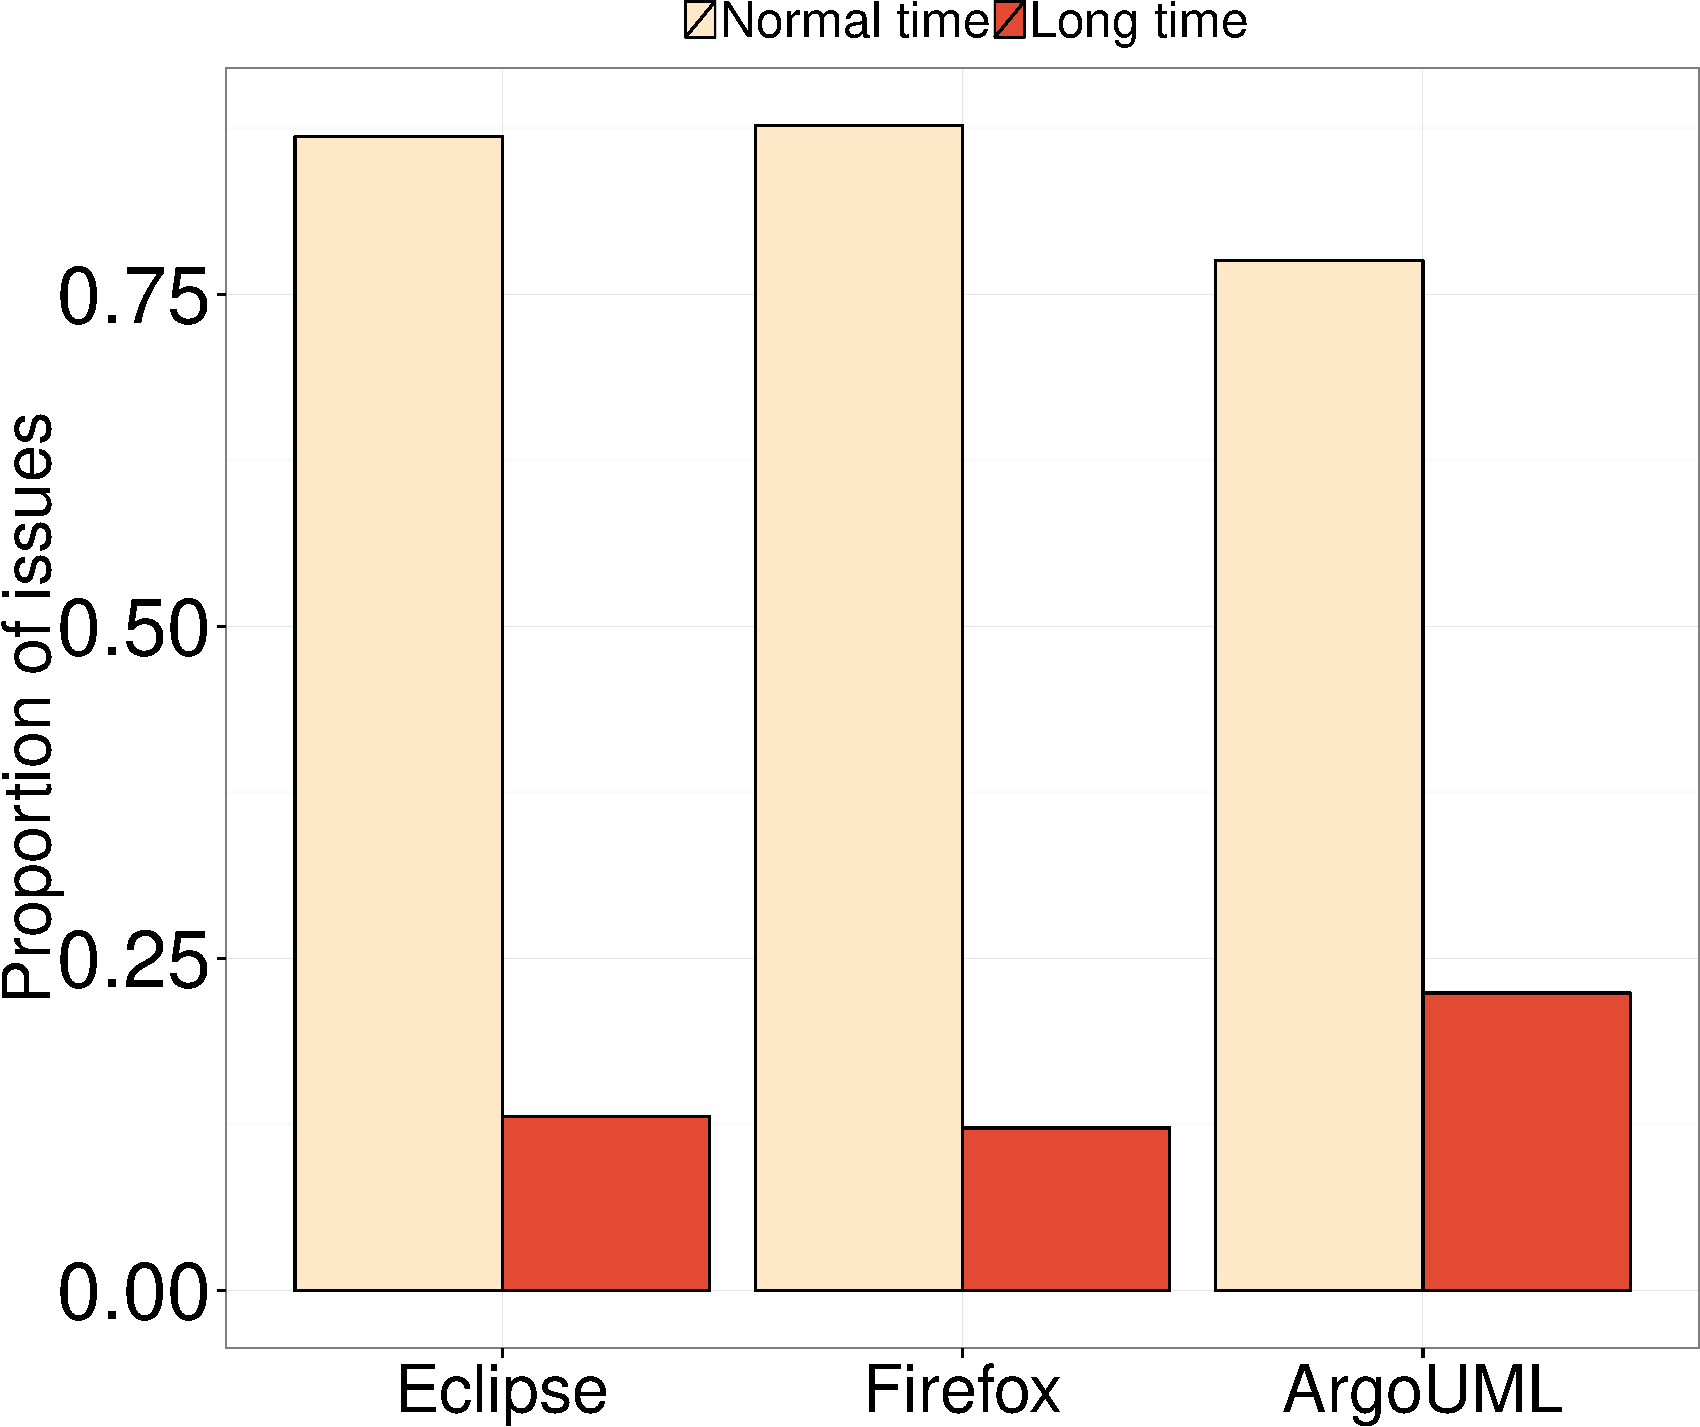
\includegraphics[width=0.80\textwidth,keepaspectratio]
	{chapters/chapter4/figures/largelydelayed_issues_per_project.pdf}
	\caption{\textbf{Addressed issues that have a prolonged delivery delay.} We present
		the proportion of addressed issues that have a prolonged
		delivery delay per project. 13\%, 12\%, and 22\% of the addressed issues
		of the Eclipse, Firefox, and ArgoUML projects have a prolonged
		\DIFdelbeginFL \DIFdelFL{integration
	time}\DIFdelendFL \DIFaddbeginFL \DIFaddFL{delivery delay}\DIFaddendFL , respectively.}
		\label{ch4:fig:largely_delayed_issues}
	\end{figure}

\hyperref[ch4:tbl:median_plus_mad]{Table}~\ref{ch4:tbl:median_plus_mad} shows
the medians and MADs for each project to identify addressed issues that have a
prolonged delivery delay. For instance, an addressed issue have a prolonged
delivery delay in the Firefox project when that issue takes more than 123 days
to be \DIFdelbegin \DIFdel{integrated}\DIFdelend \DIFaddbegin \DIFadd{delivered}\DIFaddend .
\hyperref[ch4:fig:largely_delayed_issues]{Figure}~\ref{ch4:fig:largely_delayed_issues}
shows the proportion of issues that have a prolonged delivery delay per project.
We observe that 13\%, 12\%, and 22\% of the addressed issues in the Eclipse,
Firefox, and ArgoUML projects have a prolonged delivery delay, respectively. 

\begin{table}[t!]
	\footnotesize
	\centering
	\caption{\textbf{Prolonged delivery delay thresholds.} We present the median
	delivery delay in terms of days, the MAD, and the prolonged delivery delay threshold for each project.}
	\label{ch4:tbl:median_plus_mad}
	\begin{tabular}{lrrr}
		\cline{2-4} 
		\multicolumn{1}{c}{} & \textbf{Eclipse} & \textbf{Firefox} &
		\textbf{ArgoUML}\tabularnewline
		\hline 
		\textbf{Median delivery delay} & 166 & 107 & 146\tabularnewline
		\hline 
		\textbf{Median absolute deviation} & 142 & 16 & 131\tabularnewline
		\hline 
		\textbf{Prolonged delivery delay} & $>$ 308 & $>$ 123 & $>$ 278\tabularnewline
		\hline 
	\end{tabular}
\end{table}

To train our exploratory models, we produce a dichotomous response variable $Y$,
where $Y=1$ means that an addressed issue has a prolonged delivery delay, while $Y=0$
means that the delivery delay of that issue is normal. Finally, we train
random forest models to study whether a given addressed issue is likely to have a
prolonged delivery delay. Similar to \hyperref[ch4:rq2]{RQ2}, we evaluate our models
using \textit{precision}, \textit{recall}, \textit{F-measure}, and \textit{AUC}.

\subsubsection*{RQ5: Results}

\noindent\DIFdelbegin \textit{\textbf{\DIFdel{Our models obtain F-measures from 0.79 to 0.96.}}%DIFAUXCMD
}
%DIFAUXCMD
\DIFdelend \DIFaddbegin \finding{Our models obtain F-measures from 0.79 to 0.96.}{find14}
\DIFaddend \hyperref[ch4:tbl:RFclassificationResult_ab]{Table}~\ref{ch4:tbl:RFclassificationResult_ab}
shows the performance of our exploratory models. Our models that we train for
the Eclipse project obtain the highest F-measure (0.96). On the other hand, our
models trained for the Firefox and ArgoUML projects obtain F-measures of 0.79
and 0.88, respectively. Moreover, our models obtain AUC values of 0.82 to 0.96.
Such results suggest that our models vastly outperform na\"{i}ve models, such as
random guessing (AUC value of 0.50).  \\

\begin{table}[t!]
	\footnotesize
	\centering
	\caption{\textbf{Performance of the random forest models.} The table
		shows the values of Precision, Recall, F-measure, and AUC values that
	are computed for the LOOCV of our models.}
	\label{ch4:tbl:RFclassificationResult_ab}
	\begin{tabular}{lccc}
		\cline{2-4} 
		& \textbf{Eclipse} & \textbf{Firefox} & \textbf{ArgoUML}\tabularnewline
		\hline 
		\textbf{Precision} & 0.97 & 0.99 & 0.98\tabularnewline
		\hline 
		\textbf{Recall} & 0.96 & 0.66 & 0.80\tabularnewline
		\hline 
		\textbf{F-measure} & 0.96 & 0.79 & 0.88\tabularnewline
		\hline 
		\textbf{AUC} & 0.96 & 0.82 & 0.89\tabularnewline
		\hline 
	\end{tabular}
\end{table}

\noindent\DIFdelbegin \textit{\textbf{\DIFdel{Our models obtain better F-measure values than
Zero-R.}}%DIFAUXCMD
} %DIFAUXCMD
\DIFdelend \DIFaddbegin \finding{Our models obtain better F-measure values than
Zero-R.}{find15} \DIFaddend For the Eclipse, Firefox, and ArgoUML projects, Zero-R obtain median F-measures
of 0.22, 0.22, and 0.36, respectively. Meanwhile, our explanatory models obtain
F-measures of 0.96, 0.79, and 0.88, respectively. Again, such results suggest
that our models vastly outperform na\"{i}ve classification techniques.  \\

\conclusionbox{
We are able to accurately identify whether an addressed issue is likely to have
a long delivery delay in a given project. Our models outperform na\"{i}ve
techniques, such as Zero-R and random guessing, obtaining AUC values from 0.82
to 0.96 (median).
}

\subsection{RQ6: What are the most influential attributes for                        
	identifying the issues that will suffer from a prolonged \DIFdelbegin \DIFdel{integration              
time}\DIFdelend \DIFaddbegin \DIFadd{delivery delay}\DIFaddend ?}\label{ch4:rq6}                                                                    

\subsubsection*{RQ6: Motivation} RQ6 shows that we can accurately                    
identify whether an addressed issue is likely to have a prolonged delivery delay.         
However, it is also important to understand what attributes are more influential    
when identifying addressed issues with prolonged delivery delay, \ie from which attributes 
do our models derive the most explanatory power?                                    

\subsubsection*{RQ6: Approach} Similar to \hyperref[ch4:rq4]{RQ4}, in this research
question, we analyze our explanatory models by computing the variable importance
score of the attributes.                                                                         

\subsubsection*{RQ6: Results}

\begin{figure}
	\centering
	\subfloat[Eclipse]{
		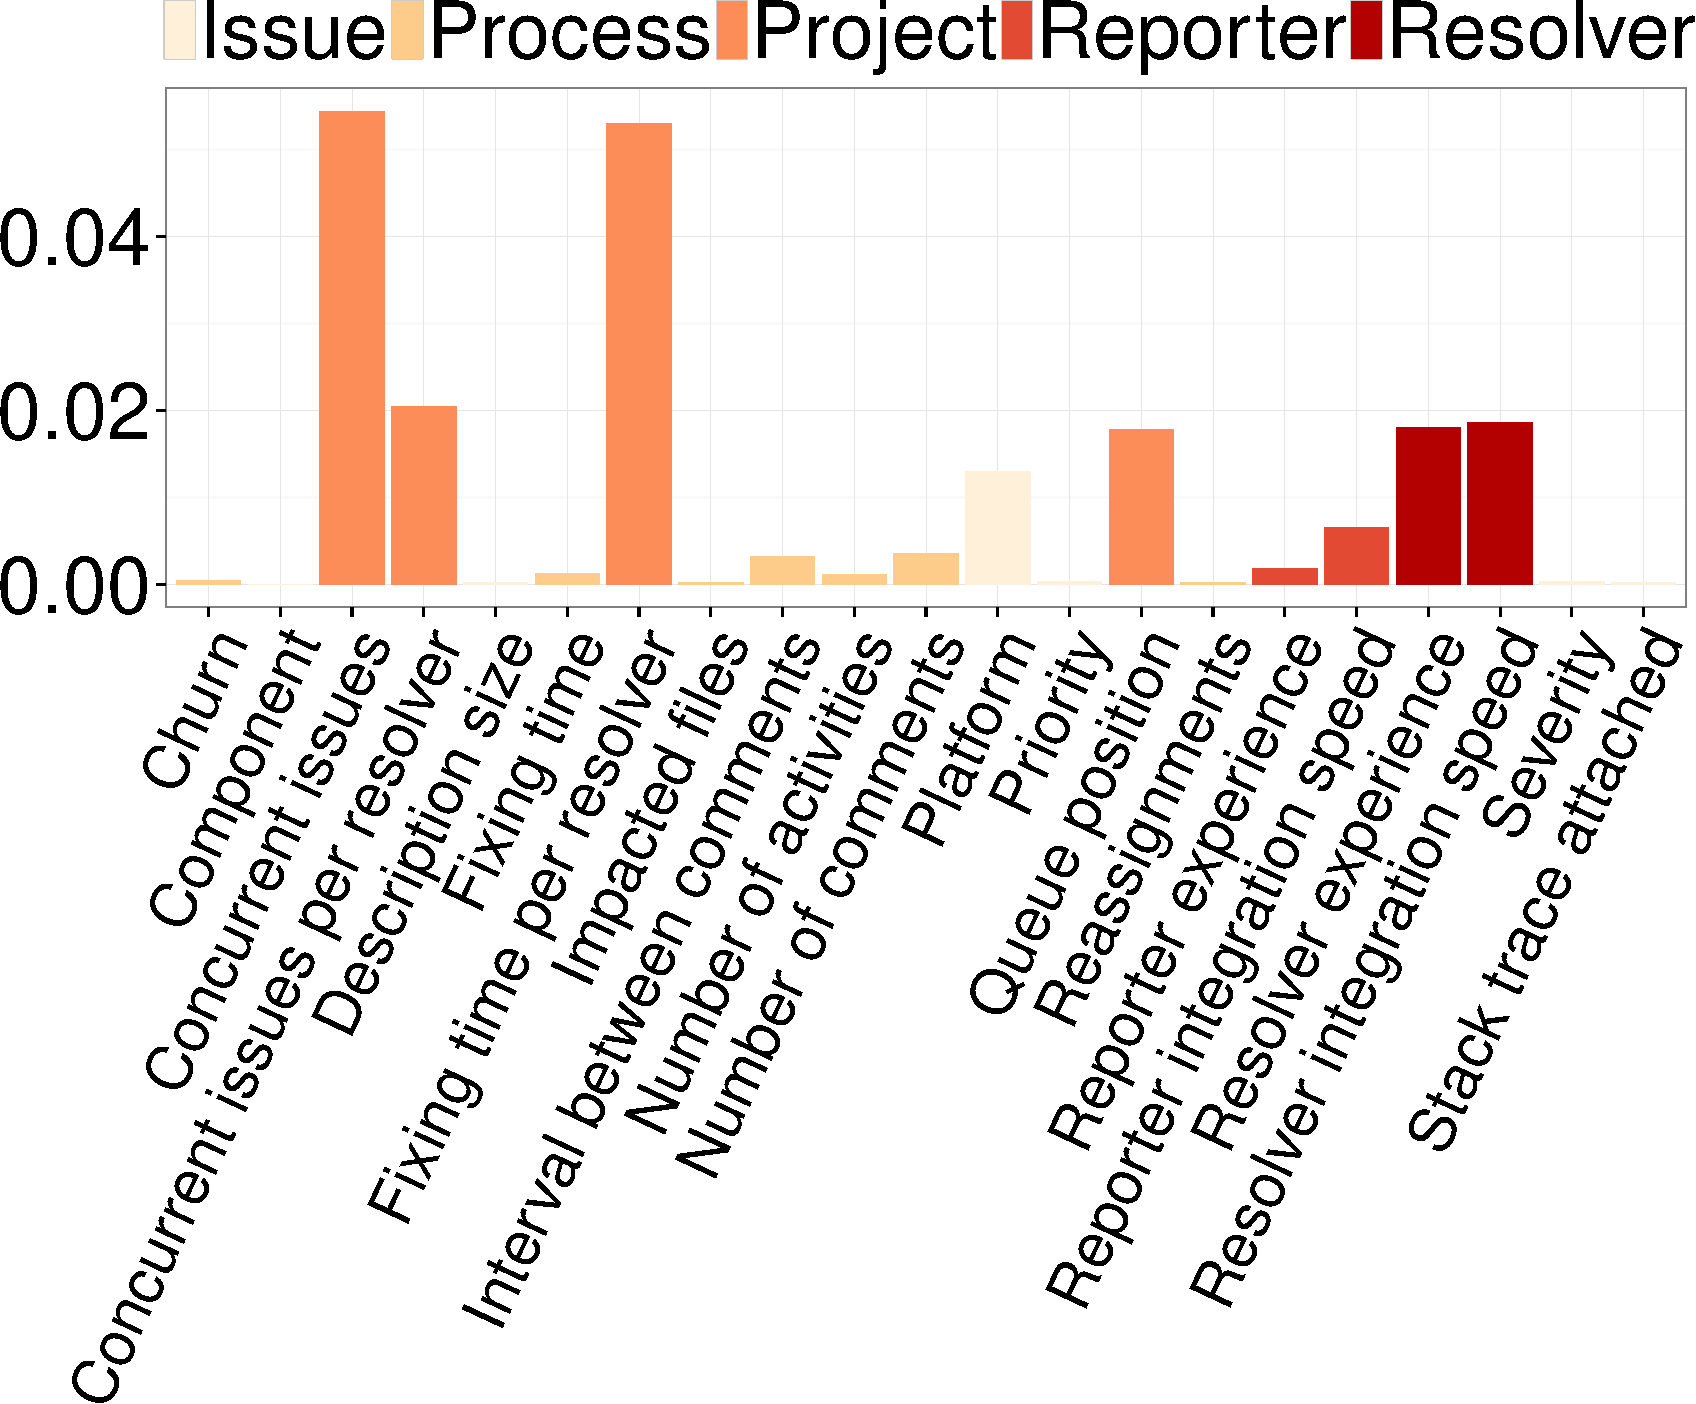
\includegraphics[width=0.50\textwidth,keepaspectratio] 
		{chapters/chapter4/figures/eclipse_loocv_varimp_long.pdf}
	\label{ch4:fig:impEclipse_ab}}

	\subfloat[Firefox]{
		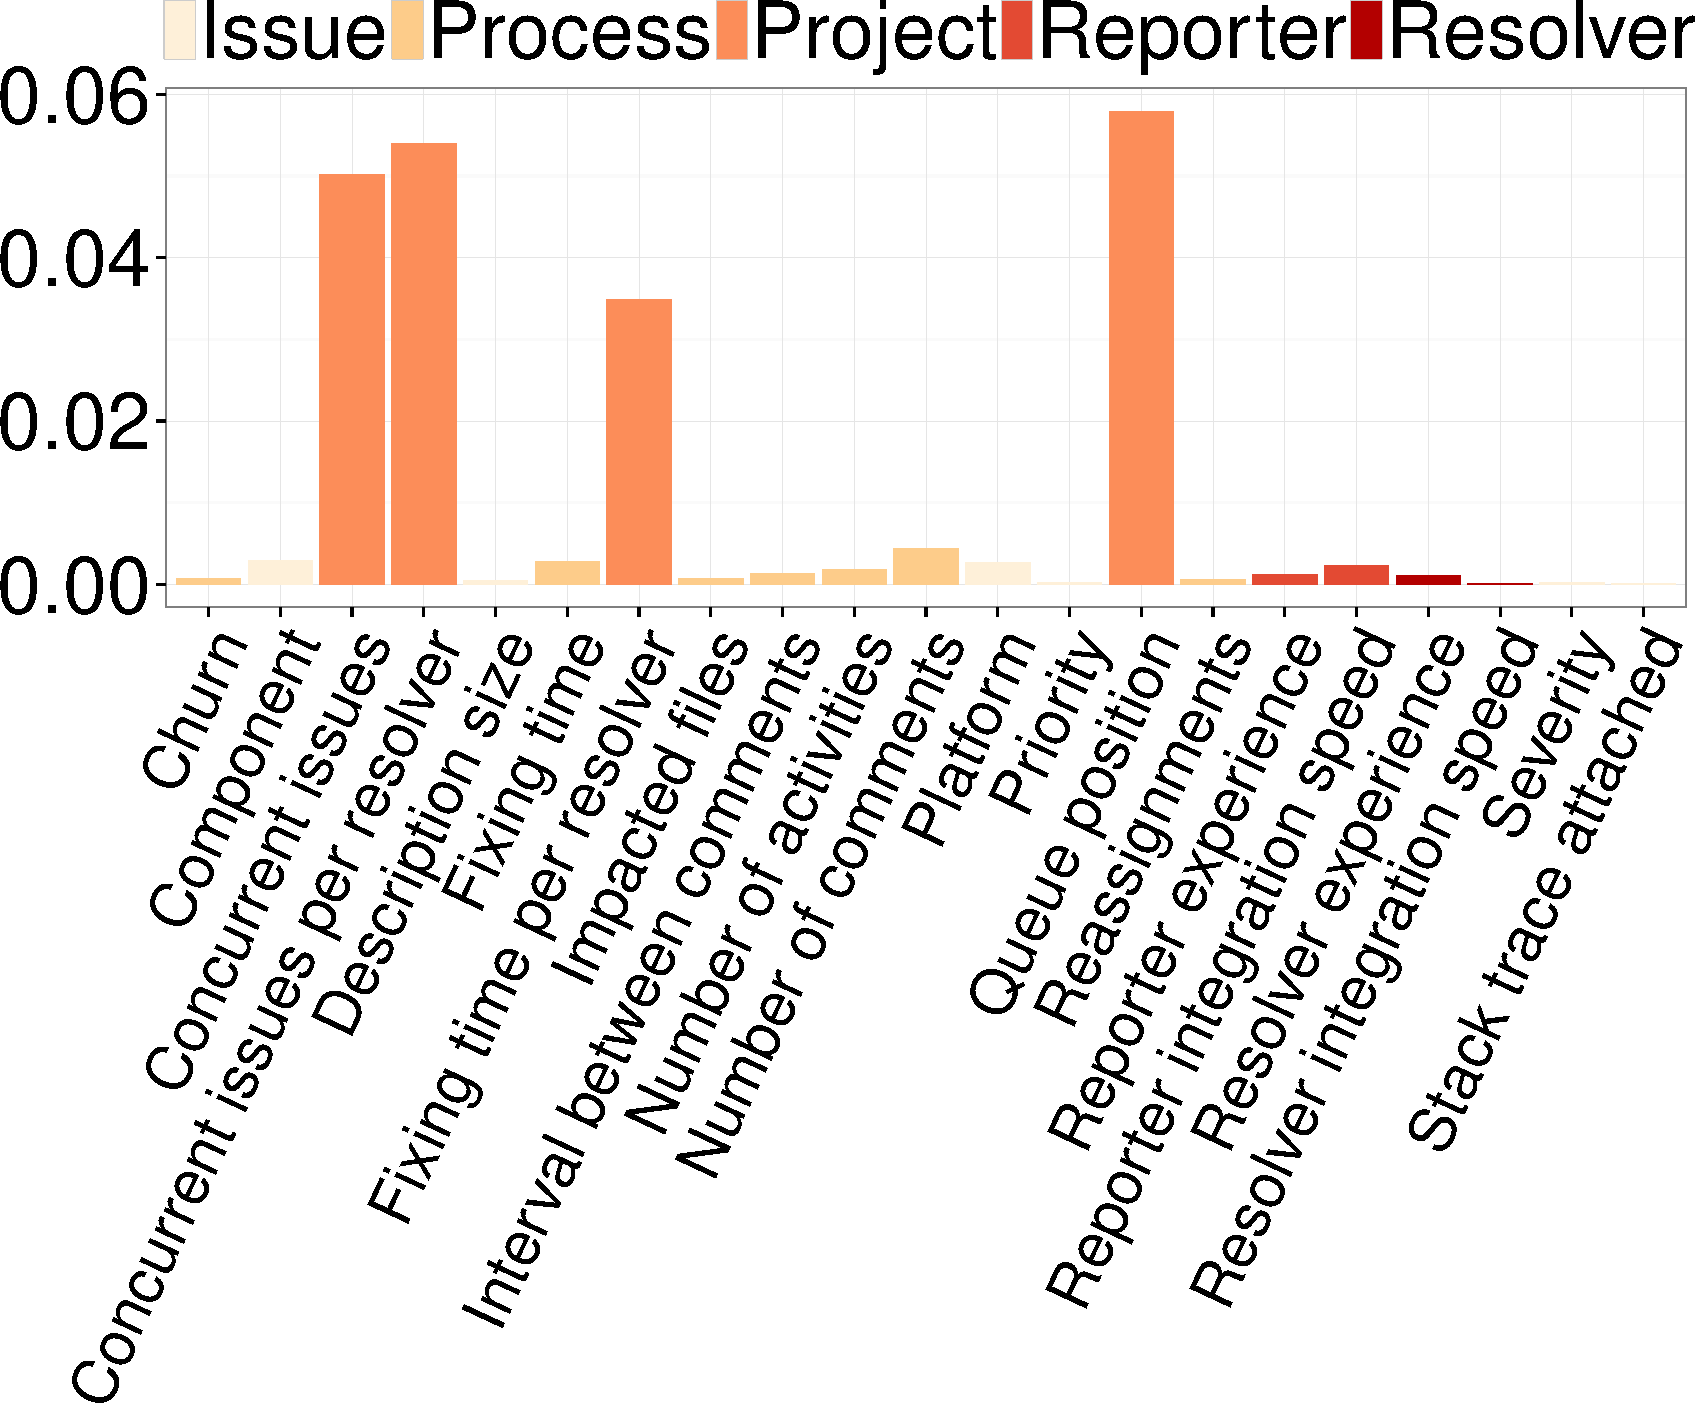
\includegraphics[width=0.50\textwidth,keepaspectratio]  
		{chapters/chapter4/figures/firefox_loocv_varimp_long.pdf}
		\label{ch4:fig:impFirefox_ab}
	}

	\subfloat[ArgoUML]{
		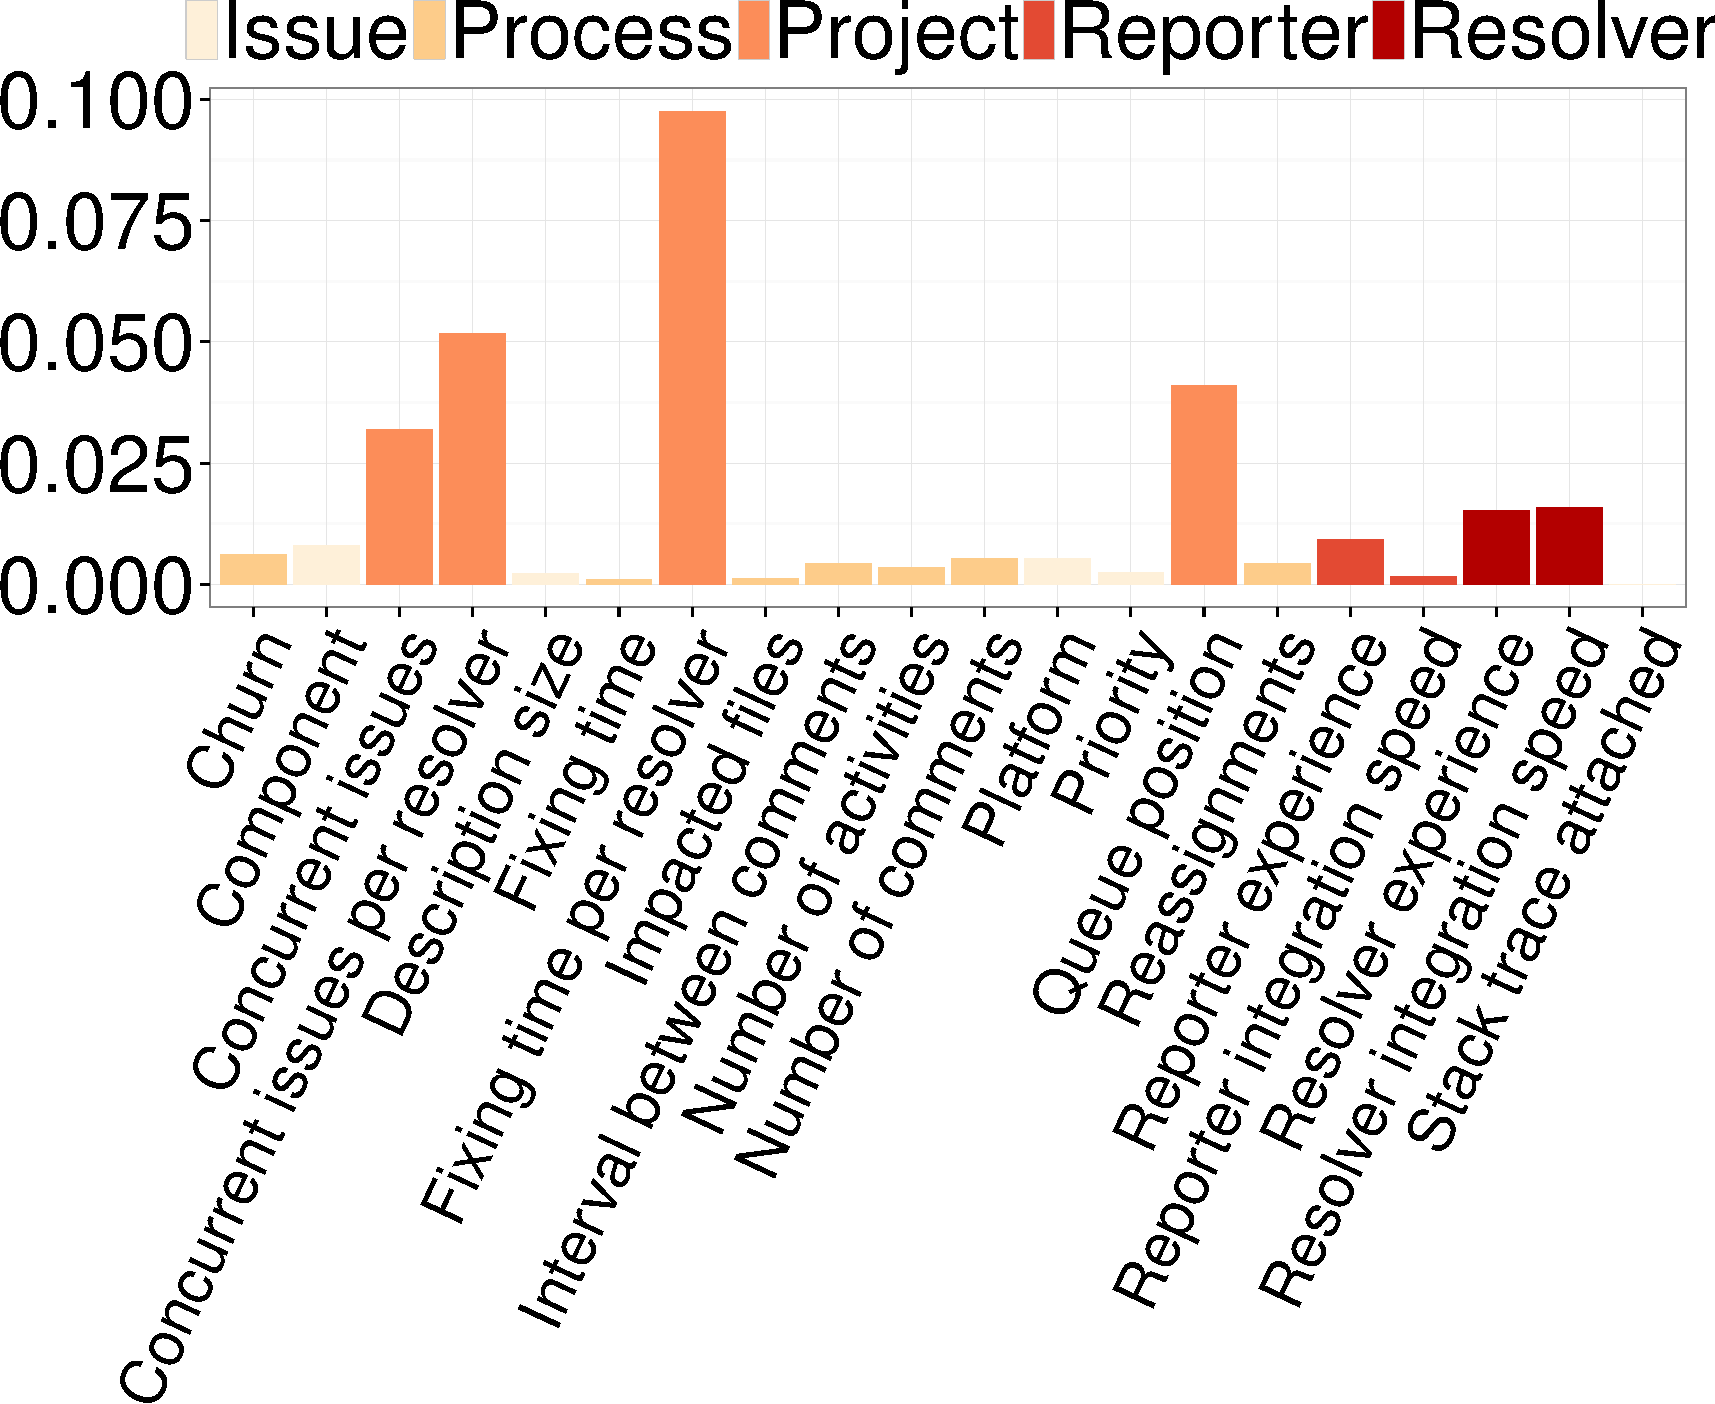
\includegraphics[width=0.50\textwidth,keepaspectratio] 
		{chapters/chapter4/figures/argouml_loocv_varimp_long.pdf}
	\label{ch4:fig:impArgo}}
	\caption{\textbf{Variable importance scores.} We show the 
	importance scores that are computed for the LOOCV of our models.}
	\label{ch4:fig:variableImportance_ab}
\end{figure}


\noindent\DIFdelbegin \textit{\textbf{%DIFDELCMD < {%%%
\DIFdel{Prolonged delivery delay is most consistently associated with
attributes of the project family.}%DIFDELCMD < }%%%
}%DIFAUXCMD
}
%DIFAUXCMD
\DIFdelend \DIFaddbegin \finding{Prolonged delivery delay is most consistently associated with
attributes of the project family.}{find16}

\DIFaddend \hyperref[ch4:fig:variableImportance_ab]{Figure}~\ref{ch4:fig:variableImportance_ab}
shows the importance scores that are computed for the LOOCV that we use to
evaluate our random forest models. We observe that the attributes that are
related to the \textit{\textbf{project}} family are the most influential
attributes in the projects. The \textit{backlog of issues} is the most
influential attribute in our Eclipse models, while \textit{queue position} and
\textit{fixing time per resolver} are the most influential attributes in our
Firefox and ArgoUML models, respectively. In addition, we observe that
attributes that are related to workload, such as the \textit{backlog of issues}
and the \textit{backlog of issues per resolver} are at least the third most
influential attributes in all of our models. Such results suggest that a
\textit{prolonged delivery delay} is associated with project-related attributes and
that the amount of addressed issues that are to be \DIFdelbegin \DIFdel{integrated }\DIFdelend \DIFaddbegin \DIFadd{delivered }\DIFaddend also plays a major
role to identify a \textit{prolonged delivery delay}. \\

\conclusionbox{Our explanatory models suggest that prolonged delivery delay is more
	closely associated with project characteristics, such as
	the \textit{backlog of issues}, \textit{queue position}, and
	\textit{fixing time per resolver}. Moreover, the backlog of issues plays an
	influential role in identifying a prolonged delivery delay in all of the studied
projects.}

